\documentclass[a4paper,makeidx,envcountchap,graybox,deutsch,ngerman,sectrefs]{svmono}
%\documentclass[envcountchap,graybox,deutsch,sectrefs]{svmono}
%%%%% eigene tempor�re Abk�rzungsliste, f�r die Zeit, bis einheitliche Schreibungen bestehen
\usepackage{tempshort}
%%  Von Springer empfohlene Pakete %% 
%%\documentclass[envcountsect,graybox,deutsch,sectrefs]{svmono}
\usepackage{chapterbib}
\usepackage{type1cm}
\usepackage[ansinew]{inputenc}
\usepackage{babel}
\usepackage[pdftex]{graphicx}  %PDF-Vektorgrafiken einbinden
\usepackage{newtxtext}         %Typischer Springer-Font
\usepackage{newtxmath}
\usepackage{multicol}
\usepackage{multirow}
\usepackage[bottom]{footmisc}  %Platziert alle Fu�noten unten  
\usepackage[nobreak]{cite}
%\usepackage{biblatex}
\usepackage{cancel}
\usepackage[absolute]{textpos}
\usepackage{pdflscape}
\usepackage{graphicx}
\usepackage{pdflscape}
\usepackage{ragged2e}
\usepackage[format=plain,
      justification=RaggedRight,
      singlelinecheck=false]
     {caption}
\usepackage{longtable}
%\usepackage{floatrow}
%\usepackage{mwe}
\usepackage[figuresright]{rotating}
\usepackage{bigints}
\let\laplace\relax  % Vermeidung der Fehlermeldung "\laplace already defined."
\usepackage{trfsigns}
%\usepackage{relsize}
\usepackage{tabulary}
%\usepackage{xcolor,colortbl}
%\usepackage[table]{xcolor}
\usepackage{blindtext}
%\usepackage{acronym}
%\usepackage{amsmath}
\usepackage{acro}
\usepackage{nomencl}


\usepackage{etoolbox}
%  Eigene Pakete %%
\usepackage{adjustbox}
\usepackage{wasysym}
\usepackage{gensymb}
\usepackage{float}
\usepackage{caption}
\usepackage[left=3cm, right=3cm, top=3cm, bottom=3cm, includeheadfoot]{geometry}

\usepackage{mathtools}   % Vermeidung der Fehlermeldung "Undefined control sequence \coloneqq."
% header and footer
\usepackage{fancyhdr}
\pagestyle{fancy}
\fancyhead{}
\fancyhead[LE,RO]\thepage
\renewcommand{\sectionmark}[1]{\markright{\thesection.\ #1}}
%\fancyhead[LO]{\nouppercase\leftmark}
%\fancyhead[RE]{\nouppercase\rightmark}
\fancyhead[LO]{\nouppercase\rightmark}
\fancyhead[RE]{\nouppercase\leftmark}
\fancyfoot{}
% svmono hat offenbar irgendwas merkw�rdig definiert, darum mu� hier verbreitert werden
%\addtolength\headwidth{25pt}
%\setlength{\headheight}{25pt}

%% Units
\usepackage{siunitx}
\sisetup{
  locale = US,
  per-mode = reciprocal, %symbol, % | reciprocal | fraction | ?
  exponent-product = \cdot,
  separate-uncertainty,
  %exponent-to-prefix,
  %prefixes-as-symbols = false,
  %list-units = brackets,% | single | repeat
  %range-units = brackets,% | single | repeat
  %multi-part-units = brackets,% | single | repeat
}
\usepackage{chngcntr}
\usepackage{booktabs}
\usepackage{slashed}
\usepackage{listings}
\usepackage{color} %red, green, blue, yellow, cyan, magenta, black, white
%\usepackage{color} %Einfache Farbendefinition -> von Graybox-Option ben�tigt
\usepackage{multirow}
\usepackage{longtable} %Tabellen �ber mehrere Seiten hinweg
\usepackage{framed} % von Graybox-Option ben�tigt
\usepackage[shortlabels]{enumitem} %Erweiterte Aufz�hloptionen
\usepackage{array}
\usepackage[xindy]{imakeidx} %Wortindex und Personenindex erstellen

\usepackage[hyphens]{url}
%\usepackage[breaklinks,colorlinks=true,linkcolor=black,urlcolor=blue,citecolor=black,filecolor=green,hyperfootnotes=false]{hyperref}
\usepackage[                                    %Hyperref erstellt ein Bookmark/Lesezeichen im PDF. siehe https://www.namsu.de/Extra/pakete/Hyperref.html
bookmarksopen=true,															%Das Lesezeichen ist ge�ffnet beim �ffnen der PDF.
bookmarksnumbered=true,                         %Zahlen werden im Bookmark angezeigt.   
plainpages=false,
pdfpagelabels,
colorlinks=true,                                %Links werden farbig dargestellt.
linkcolor=black, citecolor=black, urlcolor=cyan %Farben definieren.
]{hyperref}                                     %Sollte als letztes eingebunden werden, da es sehr viele Verweise und �nderungen erzeugt. Das Packet ist sehr stark, aber auch umfangreich ist. 
\pdfminorversion=5

\usepackage{hypcap}
\usepackage[record,section=section,stylemods={mcols},automake]{glossaries-extra}
\usepackage{glossary-longextra}
\setglossarystyle{long-name-sym-desc-loc}
\setabbreviationstyle[acronym]{long-short}

\definecolor{killA}{rgb}{.7,.3,.3}
\newcommand\killA[1]{\bgroup\color{killA}{\cancel{#1}}\egroup}
\newcommand\killB[1]{\bgroup\color{cyan!30!black}{\cancel{#1}}\egroup}
% typographisch korrekte Abk�rzungen (needs to be loaded after hyperref)
\usepackage{abbrev}
\newglossary*{bew}{Glossar}
\newglossary*{hm}{Glossar}
\newglossary*{adyn}{Glossar}
\newglossary*{kontmech}{Glossar}
\newglossary*{aero}{Glossar}
\newglossary*{edyn}{Glossar}
\newglossary*{srt}{Glossar}
\newglossary*{spo}{Glossar}
\newglossary*{optbas}{Glossar}
\newglossary*{optger}{Glossar}
\newglossary*{optatm}{Glossar}
\GlsXtrLoadResources[src={bew/gloss},type=bew]
\GlsXtrLoadResources[src={hm/gloss},type=hm]
\GlsXtrLoadResources[src={adyn/gloss},type=adyn]
\GlsXtrLoadResources[src={kontmech/gloss},type=kontmech]
\GlsXtrLoadResources[src={aero/gloss},type=aero]
\GlsXtrLoadResources[src={spo/gloss},type=spo]
\GlsXtrLoadResources[src={edyn/gloss},type=edyn]
\GlsXtrLoadResources[src={srt/gloss},type=srt]
\GlsXtrLoadResources[src={optbas/gloss},type=optbas]
\GlsXtrLoadResources[src={optger/gloss},type=optger]
\GlsXtrLoadResources[src={optatm/gloss},type=optatm]
\glssetcategoryattribute{bew}{indexname}{true}
%\renewcommand\index\newterm
%\newcolumntype{g}[1]{>{\RaggedRight\hspace{0pt}}p{#1}}
%\renewcommand\glslongextraNameAlign{g}
\renewcommand\glslongextraLocationAlign{@{\ ~\ }>{\raggedright}p{\glspagelistwidth}}
\definecolor{gls}{rgb}{.4,.4,.5}
\renewcommand*{\glstextformat}[1]{\textcolor{gls}{#1}}

%Absatzregeln
\clubpenalty = 30000 %Keine einzelnen Absatzzeilen
\widowpenalty = 30000
\setlength{\parindent}{0em} 
\newcolumntype{L}[1]{>{\raggedright\arraybackslash}p{#1}}
\newcolumntype{C}[1]{>{\centering\arraybackslash}p{#1}}
\newcolumntype{R}[1]{>{\raggedleft\arraybackslash}p{#1}}

\usepackage{xstring}

\newcommand\mfile[2]{%
\saveexpandmode\noexpandarg
\StrSubstitute{#2}{_}{\_}[\tmpname]
\restoreexpandmode
\href{MatlabDateien/\chapname/#1\tmpname}{\tmpname}}

%%% Hyperlinks zu MATLAB Dateien
%\newcommand\mlref[1]{\mfile{}{#1}}
%\newcommand\mlinclref[1]{\mfile{IncludeFolder/}{#1}}
%\newcommand\mldataref[1]{\mfile{Data/}{#1}}

%%% .. f�r ein Verzeichnis hoch
%%% . f�r aktuelle Verzeichnis
%% lokal: MatlabDateien/bew
%\newcommand\mlbewref[1]{\href{MatlabDateien/bew/#1}{#1}}
%% git: https://github.com/sn-code-inside/fingeruebungen-physik/tree/main/bew
\newcommand{\mlrefwithindex}[2]{%
  \index[mfiles]{#2}%   <-- Eintrag im M-File-Index mit aktueller Seitenzahl
  \href{https://github.com/sn-code-inside/fingeruebungen-physik/tree/main/#1/#2}{#2}%
}


%\newcommand\mlbewref[1]{\href{https://github.com/sn-code-inside/fingeruebungen-physik/tree/main/bew/#1}{#1}}
%\newcommand\mlbewdref[1]{\href{https://github.com/sn-code-inside/fingeruebungen-physik/tree/main/bew/Data/#1}{#1}}
%\newcommand\mlbewiref[1]{\href{https://github.com/sn-code-inside/fingeruebungen-physik/tree/main/bew/IncludeFolder/#1}{#1}}
%\newcommand\mlkontmechref[1]{\href{https://github.com/sn-code-inside/fingeruebungen-physik/tree/main/kontmech/#1}{#1}}
%\newcommand\mlkontmechdref[1]{\href{https://github.com/sn-code-inside/fingeruebungen-physik/tree/main/kontmech/Data/#1}{#1}}
%\newcommand\mlkontmechiref[1]{\href{https://github.com/sn-code-inside/fingeruebungen-physik/tree/main/kontmech/IncludeFolder/#1}{#1}}
%\newcommand\mlhmref[1]{\href{https://github.com/sn-code-inside/fingeruebungen-physik/tree/main/hm/#1}{#1}}
%\newcommand\mlhmdref[1]{\href{https://github.com/sn-code-inside/fingeruebungen-physik/tree/main/hm/Data/#1}{#1}}
%\newcommand\mlhmiref[1]{\href{https://github.com/sn-code-inside/fingeruebungen-physik/tree/main/hm/IncludeFolder/#1}{#1}}
%\newcommand\mladynref[1]{\href{https://github.com/sn-code-inside/fingeruebungen-physik/tree/main/adyn/#1}{#1}}
%\newcommand\mladyndref[1]{\href{https://github.com/sn-code-inside/fingeruebungen-physik/tree/main/adyn/Data/#1}{#1}}
%\newcommand\mladyniref[1]{\href{https://github.com/sn-code-inside/fingeruebungen-physik/tree/main/adyn/IncludeFolder/#1}{#1}}
%\newcommand\mledynref[1]{\href{https://github.com/sn-code-inside/fingeruebungen-physik/tree/main/edyn/#1}{#1}}
%\newcommand\mledyndref[1]{\href{https://github.com/sn-code-inside/fingeruebungen-physik/tree/main/edyn/Data/#1}{#1}}
%\newcommand\mledyniref[1]{\href{https://github.com/sn-code-inside/fingeruebungen-physik/tree/main/edyn/IncludeFolder/#1}{#1}}
%\newcommand\mloptbasref[1]{\href{https://github.com/sn-code-inside/fingeruebungen-physik/tree/main/optbas/#1}{#1}}
%\newcommand\mloptbasdref[1]{\href{https://github.com/sn-code-inside/fingeruebungen-physik/tree/main/optbas/Data/#1}{#1}}
%\newcommand\mloptbasiref[1]{\href{https://github.com/sn-code-inside/fingeruebungen-physik/tree/main/optbas/IncludeFolder/#1}{#1}}
%\newcommand\mloptspezref[1]{\href{https://github.com/sn-code-inside/fingeruebungen-physik/tree/main/optspez/#1}{#1}}
%\newcommand\mloptspezdref[1]{\href{https://github.com/sn-code-inside/fingeruebungen-physik/tree/main/optspez/Data/#1}{#1}}
%\newcommand\mloptspeziref[1]{\href{https://github.com/sn-code-inside/fingeruebungen-physik/tree/main/optspez/IncludeFolder/#1}{#1}}

\newcommand\mlbewref[1]{\mlrefwithindex{bew}{#1}}
\newcommand\mlbewdref[1]{\mlrefwithindex{bew/Data}{#1}}
\newcommand\mlbewiref[1]{\mlrefwithindex{bew/Include}{#1}}
\newcommand\mlkontmechref[1]{\mlrefwithindex{kontmech}{#1}}
\newcommand\mlkontmechdref[1]{\mlrefwithindex{kontmech/Data}{#1}}
\newcommand\mlkontmechiref[1]{\mlrefwithindex{kontmech/Include}{#1}}
\newcommand\mlhmref[1]{\mlrefwithindex{hm}{#1}}
\newcommand\mlhmdref[1]{\mlrefwithindex{hm/Data}{#1}}
\newcommand\mlhmiref[1]{\mlrefwithindex{hm/Include}{#1}}
\newcommand\mladynref[1]{\mlrefwithindex{adyn}{#1}}
\newcommand\mladyndref[1]{\mlrefwithindex{adyn/Data}{#1}}
\newcommand\mladyniref[1]{\mlrefwithindex{adyn/Include}{#1}}
\newcommand\mledynref[1]{\mlrefwithindex{edyn}{#1}}
\newcommand\mledyndref[1]{\mlrefwithindex{edyn/Data}{#1}}
\newcommand\mledyniref[1]{\mlrefwithindex{edyn/Include}{#1}}
\newcommand\mlsrtref[1]{\mlrefwithindex{edyn}{#1}}
\newcommand\mlsrtdref[1]{\mlrefwithindex{srt/Data}{#1}}
\newcommand\mlsrtiref[1]{\mlrefwithindex{srt/Include}{#1}}
\newcommand\mloptbasref[1]{\mlrefwithindex{optbas}{#1}}
\newcommand\mloptbasdref[1]{\mlrefwithindex{optbas/Data}{#1}}
\newcommand\mloptbasiref[1]{\mlrefwithindex{optbas/Include}{#1}}
\newcommand\mloptgerref[1]{\mlrefwithindex{optger}{#1}}
\newcommand\mloptgerdref[1]{\mlrefwithindex{optger/Data}{#1}}
\newcommand\mloptgeriref[1]{\mlrefwithindex{optger/Include}{#1}}
\newcommand\mloptatmref[1]{\mlrefwithindex{optatm}{#1}}
\newcommand\mloptatmdref[1]{\mlrefwithindex{optatm/Data}{#1}}
\newcommand\mloptatmiref[1]{\mlrefwithindex{optatm/Include}{#1}}


\newcommand\mlcmd[1]{\textcolor{cyan}{\texttt{#1}}}

%Grafikregeln
\graphicspath{{hm/graphs/}
							{bew/graphs/}
							{kontmech/graphs/}
							{hm/graphs/}
							{adyn/graphs/}
							{edyn/graphs/}
							{srt/graphs/}
							{kontmech/graphs/}
							{spo/graphs/}
							{aero/graphs/}
							{optbas/graphs/}
							{optger/graphs/}
							{optatm/graphs/}
							{solman/graphs/}}
\DeclareGraphicsExtensions{.pdf, .png, .jpg, .jpeg}
\def\figname{Abb}
\newcommand\figref[1]{\figname.\ \ref{abb:#1}}
\usepackage[labelfont=bf]{caption}

\usepackage{tocloft}
\usepackage{etoc}
\setlength\cftfignumwidth{30pt}

% Flatterrand links
\cftsetindents{chapter}{0em}{4em}
\cftsetindents{section}{1.5em}{4em}
\cftsetindents{subsection}{3.8em}{4em}

% flacher Rand links
%\cftsetindents{chapter}{0em}{4em}
%\cftsetindents{section}{0em}{4em}
%\cftsetindents{subsection}{0em}{4em}

\newcommand\partitle[1]{
\addcontentsline{toc}{part}{#1}
\begin{titlepage}
  %\vskip 60%\p@
  \begin{center}
    {\LARGE Finger�bungen der Physik -- #1 \par}
    \vskip 3em%
    {\large Michael Kaschke und Holger Cartarius\par}
  \end{center}
\end{titlepage}
}

%\newcommand\mlref[1]{\href{\chapname/matlab/#1}{#1}}
%\newcommand\mlinclref[1]{\href{\chapname/matlab/IncludeFolder/#1}{\color{cyan}{#1}}}

%Neue Kommandos
\def\eg{e.\,g.\  \ignorespaces}     %e.g. (im Englischen Dokument)
\newcommand{\lk}{\left(}        %gro�e runde Klammer (links)
\newcommand{\rk}{\right )}      %gro�e runde Klammer (rechts)
\newcommand{\lgk}{\left \{}     %gro�e geschweifte Klammer (links)
\newcommand{\rgk}{\right \}}    %gro�e geschweifte Klammer (rechts)
\newcommand{\lek}{\left [}      %gro�e eckige Klammer (links)
\newcommand{\rek}{\right ]}     %gro�e eckige Klammer (rechts)
\newcommand{\anf}[1]{\glqq#1\grqq}    %Deutsche Anf�hrungszeichen: \anf{}
\newcommand{\defined}{:=}				%Definition
\newcommand{\curl}{\text{\textbf{rot}}\,}	%Rotation-Operator curl()
\newcommand{\ket}[1]{|#1\rangle}		%Quantenmechanischer Zustand
\newcommand{\curvelintri}{\,\overset{\blacktriangle}{\smallfrown}}
\newcommand{\straighttri}{\blacktriangle}
\newcommand{\UT}{\text{UT}}
\newcommand{\UTC}{\text{UTC}}
\newcommand{\JD}{\text{JD}}
\newcommand{\JDE}{\text{JDE}}
\newcommand{\MJD}{\text{MJD}}
\newcommand{\TDT}{\text{TDT}}
\newcommand{\TT}{\text{TT}}
\newcommand{\NVS}{\text{Navier-Stokes-Gleichungen}}
\newcommand{\MWG}{\text{Max\-well-Gleich\-ungen}}
\newcommand{\HG}{\text{Helm\-holtz-Glei\-chung}}
\newcommand{\sHG}{\text{ska\-lare Helm\-holtz-Glei\-chung}}
\newcommand{\vHG}{\text{vek\-to\-riel\-le Helm\-holtz-Glei\-chung}}
\newcommand{\sHGn}{\text{ska\-laren Helm\-holtz-Glei\-chung}}
\newcommand{\vHGn}{\text{vek\-to\-riel\-len Helm\-holtz-Glei\-chung}}
\newcommand{\SRT}{\text{Spezielle Relativit�tstheorie}}
\newcommand{\sRT}{\text{speziellen Relativit�tstheorie}}
\newcommand{\EMW}{\text{Elek\-tro\-magne\-tische Wellen}}
\newcommand{\eMW}{\text{elek\-tro\-magne\-tische Wellen}}
\newcommand{\eme}{\text{elektromagnetische}}
\newcommand{\EMF}{\text{Elektromagnetisches Feld}}
\newcommand{\eMF}{\text{elektromagnetischen Feld}}
\newcommand{\RT}{\text{Relativit�tstheorie~}}
\newcommand{\au}{\mathrm{AE}}
\newcommand{\ET}{\text{ET}}
\newcommand{\TAI}{\text{TAI}}
\newcommand{\GMST}{\text{GMST}}
\newcommand{\LMST}{\text{LMST}}
\newcommand{\MESZ}{\text{MESZ}}
\newcommand{\KOS}{\text{Koordinatensystem }}
\newcommand{\DGL}{\text{Differentialgleichung }}
\newcommand{\NA}{\text{NA}}
\newcommand{\uA}{\text{u}}  %atomare Masseneinheit
\newcommand{\MOZ}{\text{MOZ}}
\newcommand{\grad}{\text{\textbf{grad}}\,}	%Gradient-Operator grad()
\newcommand{\uproman}[1]{\uppercase\expandafter{\romannumeral#1}}
\newcommand{\lowroman}[1]{\romannumeral#1\relax}
\newcommand\todo[1]{\textcolor{red}{TODO: #1}}
\renewcommand{\=}[1]{\stackrel{\text{#1}}{=}}  %Schrift �ber Gleich-Zeichen
\renewcommand{\d}{\partial}
\newcommand{\abs}[1]{\left\vert#1\right\vert}            %Betragsklammern
\renewcommand{\Re}{\mathrm{Re}}                          %Realteil
\renewcommand{\Im}{\mathrm{Im}}                          %Imagin�rteil
\renewcommand{\im}{\mathrm{i}}                           %Imagin�re Einheite
\newcommand{\epsi}{\varepsilon} 
\renewcommand{\exp}{\mathrm{exp}}                        %Exponentialfunktion
\newcommand{\keff}{k_\text{eff}}
\newcommand{\con}{\text{const}}
\newcommand{\conv}{\vec{const}}
\newcommand{\nL}{n_\text{L}}    %n_L Brechungsindex Linse
\newcommand{\PL}{\mathcal{P}_}  %Legendre Polynome
\newcommand{\Pl}{\mathcal{P}}   %Legendre Polynome �ltere Variante 
\newcommand{\RB}{\mathcal{R}}   %Allgemeine Radial_Bessel_Funktion
\newcommand{\ve}{\vec{e}}   %Einheitsvektor
\newcommand{\vr}{\vec{r}}   %Ortsvektor
\newcommand{\vk}{\vec{k}}   %Wellenzahlvektor
\newcommand{\vp}{\vec{p}}   %Impulsvektor
\newcommand\PLZ[2]{\mathcal{P}_{#1}^{#2}}  %zugeordnete Legendre-Funktionen 

\DeclareRobustCommand{\sB}{\tilde{\mathcal{J}}} %sph�rische Bessel-Funktion 
\DeclareRobustCommand{\sNeu}{\tilde{\mathcal{N}}} %sph�rische Neumann-Funktion 
\DeclareRobustCommand{\sHank}{\tilde{\mathcal{H}}} %sph�rische Hankel-Funktion 

\newcommand\BFu {\mathcal{J}} % Bessel-Funktion 
\newcommand\NeuFu {\mathcal{N}} % Neumann-Funktion 
\newcommand\HankFu {\mathcal{H}} % Hankel-Funktion

\newcommand\B {\mathcal{J}_\ell\lk kr \rk} % Bessel-Funktion mit \ell
\newcommand\jB {\tilde{\mathcal{J}}_\ell\lk kr \rk} %sph�rische Bessel-Funktion mit \ell
\newcommand\Neu {\mathcal{N}_\ell\lk kr \rk} %Neumann-Funktion mit \ell
\newcommand\Hank {\mathcal{H}_\ell\lk kr \rk} %Hankel-Funktion mit \ell

\newcommand{\tu}{~~\text{und}~~}   %und in Gleichungen
\newcommand{\pdv}{\frac{~\d}{\d}\frac~}   %partielle Ableitung in LGL
\newcommand{\pdV}{\frac{\d}{\d}\frac}   %partielle Ableitung in LGL

%% JK commands
 \newcommand{\CP}{\cos\phi}   
 \newcommand{\SP}{\cos\phi}   
 \newcommand{\CT}{\cos\theta}   
 \newcommand{\ST}{\sin\theta}   
 \newcommand{\U}{U \left(r,\theta\right)}

\newcommand{\artanh}{\mathrm{artanh}}
\newcommand{\textqed}{\hfill ~ $\square$}
\newcommand{\mmqed}{\tag*{$\square$}}
\newcommand{\tensor}[1]{\mathbb{#1}}			 %Tensorvariable, Matrixvariable

\newcommand{\fa}{(\textbf{a})~}
\newcommand{\fb}{(\textbf{b})~}
\newcommand{\fc}{(\textbf{c})~}
\newcommand{\fd}{(\textbf{d})~}
\newcommand{\fe}{(\textbf{e})~}
\newcommand{\ff}{(\textbf{f})~}
\newcommand{\fg}{(\textbf{g})~}

\newcommand{\iF}{im Folgenden~}
\newcommand{\iA}{im Allgemeinen~}

\newcommand{\zmu}{\mathsf{\times}~}


\newcommand{\hatr}{\hat{\vec{r}}}
\newcommand{\hbtr}{\left| \hat{\vec{r}} \right|}

\DeclareMathOperator\res{Res}
\DeclareMathOperator{\sech}{sech}
\DeclareMathOperator\sgn{sgn}
% f�r Appendix - MATLAB und Python Referenz
\newcommand{\py}{Python}
\newcommand{\rotv}{\vec{rot}\,}
\newcommand{\gradv}{\vec{grad}\,}
\newcommand{\nablav}{\vec{\nabla}\,}
\newcommand{\divv}{\mathrm{div}\,}
\newcommand{\ceil}{\mathrm{ceil}}
\newcommand{\sinc}{\mathrm{sinc}}
\newcommand{\diag}{\mathrm{diag}}
\newcommand{\sign}{\mathrm{sign}}
\newcommand{\length}{\mathrm{length}}
\newcommand{\sort}{\mathrm{sort}}
\newcommand{\summ}{\mathrm{sum}}
\newcommand{\asin}{\mathrm{asin}}
\newcommand{\acos}{\mathrm{acos}}
\newcommand{\atan}{\mathrm{atan}}
\newcommand{\prodd}{\mathrm{prod}}
\newcommand{\median}{\mathrm{mediab}}
\newcommand{\mean}{\mathrm{mean}}
\newcommand{\std}{\mathrm{std}}
\newcommand{\eye}{\mathrm{eye}}
\newcommand{\zeros}{\mathrm{zeros}}
\newcommand{\ones}{\mathrm{ones}}
\newcommand{\rand}{\mathrm{rand}}
\newcommand{\inline}{\mathrm{inline}}
\newcommand{\modd}{\mathrm{mod}}
\newcommand{\floor}{\mathrm{floor}}
\newcommand{\round}{\mathrm{round}}
\newcommand{\rem}{\mathrm{rem}}
\newcommand{\sqrtt}{\mathrm{sqrt}}
\newcommand{\triu}{\mathrm{triu}}
\newcommand{\tril}{\mathrm{tril}}
\newcommand{\size}{\mathrm{size}}
\newcommand{\dett}{\mathrm{det}}
\newcommand{\rect}{\mathrm{rect}}
\newcommand{\OTF}{\mathrm{OTF}}
\newcommand{\inv}{\mathrm{inv}}
\newcommand{\rank}{\mathrm{rank}}
\newcommand{\rref}{\mathrm{rref}}
\newcommand{\eig}{\mathrm{eig}}
\newcommand{\poly}{\mathrm{poly}}
\newcommand{\lu}{\mathrm{lu}}
\newcommand{\qr}{\mathrm{qr}}
\newcommand{\R}{\mathbb{R}}
\newcommand{\quaddd}{\mathrm{quad}}
\newcommand{\fzero}{\mathrm{fzero}}
\newcommand{\roots}{\mathrm{roots}}
\newcommand{\odezd}{\textcolor{mygreen}{\texttt{ode23}}}
\newcommand{\odevf}{\textcolor{mygreen}{\texttt{ode45}}}
\newcommand{\odeeds}{\textcolor{mygreen}{\texttt{ode13s}}}
\newcommand{\odeefs}{\textcolor{mygreen}{\texttt{ode15s}}}
\newcommand{\ddezd}{\textcolor{mygreen}{\texttt{dde23}}}
\newcommand{\onlineZ}{online verf�gbaren Zusatzmaterialien{}}
%\newcommand{\MKc}{\url{https://kaschke-medtec.de/fingeruebungen.html}{}}
\newcommand{\MKc}{\url{https://www.fingeruebungen-physik.de}{}}
\newcommand{\linklsg}{\href{https://www.fingeruebungen-physik.de}{\textcolor{blue} {$\rightarrow$ L�sungsteil.}}}
\newcommand{\githubSN}{\url{https://github.com/sn-code-inside/fingeruebungen-physik}{}\,\,}

\newcommand{\PSF}{\mathrm{PSF}} %PSF
\newcommand{\FT}{\mathcal{F}} %Fourier-Transformierte
\newcommand{\iFT}{\mathcal{F}^{-1}} %inverse Fourier-Transformierte
\newcommand{\KFF}{Kugel\-fl�\-chen\-funk\-tio\-nen~} %Kugelfl�chenfunktionen
\newcommand{\HH}{Hansen-\-Har\-mo\-nics~} %Hansen-Harmonics
\newcommand{\TE}{^\mathrm{(TE)}} %Transversal elektrisch
\newcommand{\TM}{^\mathrm{(TM)}} %Transversal magnetisch
\newcommand{\sumlm}{\sum\limits_{l=0}^\infty \sum\limits_{m=-l}^l} %Summe �ber l,m KFF

% Aufz�hlung der L�sungen der Teilaufgaben
\newlist{subprobs}{enumerate}{1}
\setlist[subprobs]{
  label= \textbf{\textit{Teilaufgabe}} \textbf{\textit{\arabic*:}} \protect\thissubprob,
  ref=\arabic*, itemsep=\baselineskip, align=left}
\newcommand{\subprob}[1]{
  \def\thissubprob{\textbf{\textit{#1}}}\item ~\vspace{0.2\baselineskip} \newline}


%%%%%%%%%%%%%%%%%%%%%%%%%%%%%%%%%%%%%%%%%%%%%%%%%%%%%%%%%%%%%%%%%%%%%%%%
% Abk�rzungen, Formelzeichen

\makenomenclature
\renewcommand{\nomname}{}

\renewcommand{\nomgroup}[1]{%
  \ifthenelse{\equal{#1}{L}}{\item[]\vspace{0.4\baselineskip}\item[\bfseries Lateinische Symbole]}{%
  \ifthenelse{\equal{#1}{G}}{\item[]\vspace{0.6\baselineskip}\item[\bfseries Griechische Symbole]}{%
  \ifthenelse{\equal{#1}{O}}{\item[]\vspace{0.6\baselineskip}\item[\bfseries Indizes und Operatoren]}{}}}%
}

\newif\iffirstnomgroup
\firstnomgrouptrue

\renewcommand{\nomgroup}[1]{%
  \iffirstnomgroup
    \global\firstnomgroupfalse
  \else
    \item[]\vspace{0.6\baselineskip}%
  \fi
  \item[\bfseries
    \ifthenelse{\equal{#1}{L}}{Lateinische Symbole}{%
    \ifthenelse{\equal{#1}{G}}{Griechische Symbole}{%
    \ifthenelse{\equal{#1}{O}}{Indizes und Operatoren}{}}}%
  ]%
  \item[]\vspace{0.2\baselineskip}%
}

\setlength{\nomitemsep}{0.25\baselineskip}

\makeatletter
\renewenvironment{thenomenclature}[1][\nomlabelwidth]{%
  \nompreamble
  \setnomtableformat{lp{0.8\textwidth}sp{0.5\textwidth}@{}l}
  \setlength{\labelsep}{1.8em}
  \list{}{%
    \labelwidth#1%
    \leftmargin\labelwidth
    \advance\leftmargin\labelsep
    \itemsep\nomitemsep
    \let\makelabel\nomlabel
  }%
}{%
  \endlist
  \nompostamble
}
\makeatother

% Gemeinsame Breite der linken Spalte
\newlength{\verzlabelwidth}
\setlength{\verzlabelwidth}{2.5cm}


%%%%%%%%%%%%%%%%%%%%%%%%%%%%%%%%%%%%%%%%%%%%%%%%%%%%%%%%%%%%%%%%%%%%%%%%%%%%%%%%%%%%%%%%%%%%%%%%%%


\definecolor{mygreen}{RGB}{28,172,0} % color values Red, Green, Blue
\definecolor{myblue}{RGB}{28,28,172}
\definecolor{myyellow}{RGB}{237,162,13}
\definecolor{shadecolor}{gray}{0.95}
\definecolor{mylilas}{RGB}{170,55,241}

\renewenvironment{example}[1]{
\refstepcounter{example}\par\medskip
\begin{shaded} 
%\begin{samepage}
 
\noindent{\color{mygreen} \rule[3pt]{\textwidth}{0.3mm}}
\begin{tabular}{>{\arraybackslash}m{1cm}>{\arraybackslash}m{17cm}}

\includegraphics[width=8mm]{example.pdf}&
\noindent \textbf{\textit{Beispiel~\theexample: {#1}}}
\end{tabular}
\noindent{\color{mygreen} \rule[3pt]{\textwidth}{0.2 mm}}
%\end{samepage}
}{\end{shaded}
\vspace{-1cm}\noindent{\color{mygreen} \rule{\textwidth}{0.3 mm}}
} 

%%%%%%%%%%%%%%%%%%%%%%%%%%%%%%%%%%%%%%%%%%%%%%%%%%%%%%%%%%%%%%%

\newenvironment{infobox}[1]{
     \begin{shaded} 
     \begin{samepage}
\noindent{\color{myblue} \rule[3pt]{\textwidth}{0.3 mm}}
\begin{tabular}{>{\arraybackslash}m{1cm}>{\arraybackslash}m{17cm}}

\includegraphics[width=6mm]{info.pdf}&
%\noindent \textbf{\textit{~Infobox:~ {#1}}} 
\noindent \textbf{\textit{~ {#1}}} 
\end{tabular}
\noindent{\color{myblue} \rule[3pt]{\textwidth}{0.2 mm}}
     \end{samepage}
}{\end{shaded}
\vspace{-1cm}\noindent{\color{myblue} \rule{\textwidth}{0.3 mm}}
} 


\newenvironment{merksatz}[1]{
\begin{shaded} 
     %\begin{samepage}
\noindent{\color{myyellow} \rule[3pt]{\textwidth}{0.3 mm}}
\begin{tabular}{>{\arraybackslash}m{1cm}>{\arraybackslash}m{17cm}}

\includegraphics[width=6mm]{merke.pdf}&
%\noindent \textbf{\textit{~Merke:~ {#1}}}
\noindent \textbf{\textit{~ {#1}}}
\end{tabular}
\noindent{\color{myyellow} \rule[3pt]{\textwidth}{0.2 mm}}
     %\end{samepage}
}{\end{shaded}
\vspace{-1cm}\noindent{\color{myyellow} \rule{\textwidth}{0.3 mm}}
}

%%%%%%%%%%%%%%%%%%%%%%%%%%%%%%%%%%%%%%%%%%%%%%%%%%%%%%%%%%%%%%%


\newenvironment{nebenrechnungNeu}[1]{
\begin{shaded} 
     \begin{samepage}
\noindent{\color{black} \rule[3pt]{\textwidth}{0.3 mm}}
\begin{tabular}{>{\arraybackslash}m{1cm}>{\arraybackslash}m{17cm}}
%
\includegraphics[width=6mm]{nr.pdf}&

\includegraphics[width=6mm]{info.pdf}&
\noindent \textbf{\textit{~Nebenrechnung:~ {#1}}}
\end{tabular}
\noindent{\color{black} \rule[3pt]{\textwidth}{0.2 mm}}
     \end{samepage}
}{\end{shaded}
\vspace{-1cm}\noindent{\color{black} \rule{\textwidth}{0.3 mm}}
}

\newenvironment{nebenrechnung}[1]{
\begin{shaded} 
\begin{samepage}
\noindent\textbf{Nebenrechnung: \\} 
\noindent{\color{black} \rule{0.1\columnwidth}{0.2mm} \\}
\end{samepage}
}{\end{shaded}
\noindent{\color{black} \rule{0.1\columnwidth}{0.2mm} \\}
} % or snugshade
\definecolor{shadecolor}{gray}{0.95}
\definecolor{mygreen}{RGB}{28,172,0} % color values Red, Green, Blue
\definecolor{mylilas}{RGB}{170,55,241}


\lstset{language=Matlab,%
    %basicstyle=\color{red},
    %basicstyle={\linespread{0.9}\ttfamily},
    basicstyle=\footnotesize\ttfamily,
    breaklines=true,%
    morekeywords={matlab2tikz},
    keywordstyle={\small \color{mygreen}},%
    morekeywords=[2]{1}, keywordstyle=[2]{\small\color{black}},
    identifierstyle={\small \color{black}},%
    stringstyle={\small\color{mylilas}},
    commentstyle={\small\color{mylilas}},%
    showstringspaces=false,%without this there will be a symbol in the places where there is a space
    numbers=left,%
    numberstyle={\tiny \color{black}},% size of the numbers
    numbersep=9pt, % this defines how far the numbers are from the text
    emph=[1]{for,end,else,break, function},emphstyle=[1]\small \color{blue}, %some words to emphasise
    emph=[2]{odeset},emphstyle=[2]\small \color{mygreen}, %some words to emphasise
    %emph=[2]{word1,word2}, emphstyle=[2]{style},    
}

%\bibliographystyle{spphys.bst}

%Trennregeln f�r spezielle Worte
%\hyphenation{Fresnel \matlab �qui-nok-ti-um}

\DeclareSIUnit\erg{erg}
\DeclareSIUnit\cal{cal}
\DeclareSIUnit\celsius{C}
\DeclareSIUnit\m{M}
\DeclareSIUnit\kel{K^{-4}}

%Stichwort- und Personenverzeichnis
\makeindex[title=Stichwortverzeichnis] % Create the default index
\makeindex[name=personen,title=Personenverzeichnis] % Create an index named 'personen'
\newcommand{\indexp}[1]{\index[personen]{#1}}
\makeindex[name=mfiles,title=MATLAB-Skriptverzeichnis,columns=2]

% list of exercises
\newcommand{\loxname}{\Large �bungsverzeichnis}  % einheitliche Gr��e Large
\newlistof[chapter]{prob}{lox}\loxname
\newcommand\uebung[3][]{\label{prob:#2}%
\addcontentsline{lox}{prob}{\protect\numberline{}{\probRef{#2}:~#3#1}}%
\textbf{#1#3}\\[\baselineskip]}
\makeatletter
\renewcommand{\l@prob}{\@dottedtocline{1}{0em}{0em}}
\makeatother
\newcommand\einfach{\uebung[~$\ast$~~]}
\newcommand\mittel{\uebung[~$\ast\,\ast$~~]}
\newcommand\schwierig{\uebung[~$\ast\,\ast\,\ast$~~]}
\newcommand\zusatz{\uebung[~$\ast\,\ast\,\ast\,!$~~]}
%\newcommand\einfach{\uebung[~\textbf{*}~~]}
%\newcommand\mittel{\uebung[~\textbf{*\,*}~~]}
%\newcommand\schwierig{\uebung[~\textbf{*\,*\,*}~]}
%\newcommand\zusatz{\uebung[~\textbf{*\,*\,*\,!}~~]}
\usepackage[atend]{bookmark}
%\BookmarkAtEnd{%
%\bookmarksetup{startatroot}\bookmark[level=0,named=\loxname]{}}

% Einheitliche �berschrift
\newcommand\verzeichnisueberschrift[1]{\section*{#1}}
\newcommand\kapitel[1]{Kapitel \ref{kap:#1}}
\newcommand\kap[1]{Kap. \ref{kap:#1}}


% Acronyms

\acsetup{
  list/name     = Abk�rzungsverzeichnis,
  list/template = tabular
}

\DeclareAcronym{NASA}{short = NASA, long  = National Aeronautics and Space Administration}
\DeclareAcronym{ESO}{short = ESO, long  = European Southern Observatory}

\DeclareAcronym{ccd}{short = CCD, long  = Charge-Coupled Device}
\DeclareAcronym{otf}{short = OTF, long  = Optical Transfer Function}
\DeclareAcronym{tmm}{short = TMM, long  = Transfermatrix-Methode}
\DeclareAcronym{tmft}{short = TMFT, long  = Thin Film Matrix Theory}
\DeclareAcronym{ar}{short = AR, long  = Anti-Reflexion}
\DeclareAcronym{cgh}{short = CGH, long  = Computer Generated Hologramm}
\DeclareAcronym{grin}{short = GRIN, long  = Gradient Index}
\DeclareAcronym{vat}{short = VAT, long  = Value Averaging Theory}
\DeclareAcronym{fem}{short = FEM, long  =  Finite Elemente Methode}
\DeclareAcronym{rcwa}{short = RCWA, long  = Rigorous Coupled Wave Theory}
\DeclareAcronym{tdtd}{short = FDTD, long  = Finite Difference Time Domain}
\DeclareAcronym{adc}{short = ADC, long  = Analog-Digital-Converter}
\DeclareAcronym{psf}{short = PSF, long  = Punktspreizfunktion (Point Spread Function)}
\DeclareAcronym{apsf}{short = APSF, long  = Amplitudenpunktspreizfunktion (Amplitude Point Spread Function)}
\DeclareAcronym{fwhm}{short = FWHM, long  = Full Width Half Maximum}

\DeclareAcronym{pd}{short = PD, long  =  Photodiode}
\DeclareAcronym{pmt}{short = PMT, long  =  Photomultiplier Tube}
\DeclareAcronym{apd}{short = APD, long  =  Avalanche Photodiode}
\DeclareAcronym{spad}{short = SPAD, long  =  Single-Photon-Avalanche Photodiode}
\DeclareAcronym{spcd}{short = SPCD, long  =  Single-Photon-Count Detection}
\DeclareAcronym{cmos}{short = CMOS, long  =  Complementary Metal-Oxide-Semiconductor}
\DeclareAcronym{mcp}{short = MCP, long  =  Mikrokanalplatte (Micro Channel Plate)}
\DeclareAcronym{snr}{short = SNR, long  =  Signal-Rausch-Verh�ltnis (Signal Noise Ratio)}
\DeclareAcronym{lsm}{short = LSM, long  =  Laser-Raster-Mikroskopie (Laser-Scanning-Microscopy)}
\DeclareAcronym{ics}{short = ICS, long  =  Infinity Corrected System}
\DeclareAcronym{dic}{short = DIC, long  =  Differentielle Interferenzkontrast (Differential Interference Contrast)}

\DeclareAcronym{palm}{short = PALM, long  =  Photo-Activated Localization Microscopy}
\DeclareAcronym{sim}{short = SIM, long  =  Structured Illumination Microscopy}
\DeclareAcronym{sted}{short = STED, long  =  Stimulated Emission Depletion}
\DeclareAcronym{storm}{short = STORM, long  =  Stochastic Optical Reconstruction Microscopy}

\DeclareAcronym{aps}{short = APS, long  =  Advanced Photo System}
\DeclareAcronym{mft}{short = MFT, long  =  Micro Four Thirds}
\DeclareAcronym{dof}{short = DOF, long  =  Depth of Field}
\DeclareAcronym{fov}{short = FOV, long  =  Field ov View}
\DeclareAcronym{mp}{short = MP, long  =  Mega Pixel}



%-------------------------------------------------------
% Abk�rzungen
% ------------------------------------------------------
\begin{document}
% customize prob and sol in svmono
\makeatletter
%\counterwithin*{chapter}{part}

\spn@wtheorem{prob}{\bgroup\exercisename\egroup}{\bfseries}{\rmfamily}
\makeatother
\renewenvironment{sol}[1]{\par\addvspace{6pt}\noindent\phantomsection{\textbf{L�sung zu \ref{#1}}} \ignorespaces}{\par\addvspace{6pt}}
\newcommand\probRef[1]{�bung \ref{prob:#1}}
\renewcommand\probref[1]{\textbf{\probRef{#1}}}
\newcommand\lsgref[1]{L�sung \ref{lsg:#1}}

%\newcommand\sbullet[1][.5]{\mathbin{\vcenter{\hbox{\scalebox{#1}{$\bullet$}}}}}




\setcounter{table}{0}



\thispagestyle{plain}%\mp
\restoregeometry 
\begin{textblock}{3}(0,0)
\includegraphics{BuchtitelseiteWB5.pdf}
\end{textblock}
\leavevmode
\newpage 
\thispagestyle{empty}
\quad 
\newpage
\pagestyle{fancy}

\author{Michael Kaschke, Michael Kempe   \\
und Michael Totzeck }
\title{Finger�bungen der Physik\\ \\
Band V \\ \\ Optik \\ \\ Workbook\\}

\subtitle{Ein Lehr- und �bungsbuch mit im Studium selten behandelten Kapiteln der Physik und ausf�hrlich numerisch behandelten Problemen in \matlab- und \py- Programmen. \\
\smallskip
Unter Mitwirkung von Holger Cartarius.}
\smallskip
\maketitle

\begin{dedication}
\;\;\;To be completed.\\
\medskip
\textsc{Michael Kaschke, Michael Kempe und  Michael Totzeck}\\ 
\medskip
\medskip
\end{dedication}
\frontmatter%%%%%%%%%%%%%%%%%%%%%%%%%%%%%%%%%%%%%%%%%%%>

%\include{vorwort5}

\clearpage
\pdfbookmark[1]{Inhaltsverzeichnis}{toc}
\tableofcontents
\setcounter{tocdepth}{3}

\mainmatter%%%%%%%%%%%%%%%%%%%%%%%%%%%%%%%%%%%%%%%%%%>


%\newpage 
%\setcounter{tocdepth}{4}
%\pdfbookmark[0]{Inhaltsverzeichnis}{toc}
%\tableofcontents

%%%%%%%%%%%%%%%%%%%%%%%%%%%%%%%%%%%%%%%%%%%%%%%%

%\newcounter{fmpg}\setcounter{fmpg}{\arabic{page}}

%% Ab hier die Zusammenfassung von Band I bis Band IV

%\phantomsection
%\addcontentsline{toc}{part}{Zusammenfassung Inhalt Band I - Band IV}
%\thispagestyle{empty}
  %\begin{flushright}
    %\LARGE
    %\textbf{Inhalt von Band I - Band IV \\}
  %\end{flushright}
  %\vspace*{\fill}
%\newpage

%\begingroup
\let\cleardoublepage\relax
\chapter{Physik der Bewegung von K�rpern (Zusammenfassung)}\label{chap:bew}
\def\chapname{bew}

\begin{minipage}{0.5\textwidth}
\includegraphics[width=\textwidth]{Pendeluhr.jpg}
%
\includegraphics[width=\textwidth]{Platzhalter.pdf}
\end{minipage}
\medskip
\begin{minipage}{0.5\textwidth}
\begin{flushright}
\small
\emph{Nichts ist �lter in der Natur\\
als die Bewegung.\\}
\medskip
Galileo Galilei (1564--1642)\\
in seinen Discorsi \\
\medskip
\medskip
\emph{Zustand ist ein albernes Wort;\\
weil nichts steht und\\
alles beweglich ist.\\}
\medskip
Johann Wolfgang von Goethe (1749--1832)
\normalsize
\end{flushright}
\end{minipage}

\section*{Zusammenfassung des Inhaltes von Kapitel 1 aus Band I -- Mechanik}\label{kap:bew_zusammenfassung}

Die abgebildete alte Pendeluhr ist ein sch�nes Beispiel eines physikalischen Pendels\index{Pendel!physikalisches}.\\
Viele Physiker haben sich �ber Jahrhunderte hinweg mit der Theorie des Pendels und verschiedener Pendelformen besch�ftigt.
Das Pendel hat in der Geschichte der Menschheit �ber lange Zeit hinweg eine wesentliche Rolle bei der Zeitmessung gespielt.
Sp�ter sollte der harmonische Oszillator\index{Oszillator!harmonischer} als Modell eines Pendels sogar bei der Entwicklung der Quantenmechanik bedeutend werden.
Auch Philosophen und K�nstler wurden vielfach von den Schwingungen des Pendels inspiriert. In den �bungen und Beispielen dieses Kapitels werden deshalb auch eine Reihe von Pendeln betrachtet, an denen sich eine gro�e Bandbreite der physikalischen Methoden anwenden und vertiefen l�sst, insbesondere auch das Arbeiten mit Erhaltungss�tzen\index{Erhaltungssatz} und das L�sen von gew�hnlichen Differentialgleichungen\index{Differentialgleichung!gew�hnliche}.\\
Ebenso eignen sich mechanische Spielzeuge, wie der Kreisel\index{Kreisel}, um verschiedene grundlegende Begrifflichkeiten der Mechanik nach Newton\indexp{Newton, Sir Isaac}\footnote{Sir Isaac Newton (1643--1727) war einer der bedeutendsten Naturforscher aller Zeiten. Er formulierte die Gravitations- und Bewegungsgesetze und entwickelte fast gleichzeitig mit dem deutschen Universalgelehrten Leibniz (1646--1716) die Infinitesimalrechnung. Newtons \emph{Principia} werden als eines der wichtigsten wissenschaftlichen Werke angesehen.} (Newtonsche Mechanik)\index{Newtonsche Mechanik} einzuf�hren und an einer Vielfalt physikalischer Ph�nomene didaktisch eindrucksvoll zu erkl�ren und zu visualisieren. 
Selbst gro�e Physiker wie Einstein\footnote{Albert Einstein\indexp{Einstein, Albert} (1879--1955) war einer der bedeutendsten Physiker der Geschichte.
Seine Forschungen zu Raum und Zeit sowie zum Wesen der Gravitation\index{Gravitation} haben unser modernes Weltbild ma�geblich gepr�gt.} haben sich nicht nur in ihrer Kindheit mit diesen Spielzeugen besch�ftigt.
Sommerfeld\footnote{Arnold Sommerfeld\indexp{Sommerfeld, Arnold} (1868--1951) war ein bedeutender deutscher theoretischer Physiker, der sowohl als Forscher, als auch als akademischer Lehrer hoch anerkannt war.
Besondere Verdienste erwarb er sich durch die Anwendung fortschrittlicher mathematischer Methoden auf physikalische und technische Probleme.} schrieb mit seinem Lehrer Felix Klein\indexp{Klein, Felix Christian}\footnote{Felix Christian Klein (1849--1925) war ein deutscher Mathematiker, der im 19.~Jahrhundert bedeutende Fortschritte vor allem in der Geometrie erzielte. Klein besch�ftigte sich mit der Funktionentheorie und engagierte sich sehr f�r die Mathematikdidaktik.} das noch heute als Standard betrachtete Werk �ber die Theorie des Kreisels\footnote{F. Klein und A. Sommerfeld, \textit{�ber die Theorie des Kreisels}, Teubner Leipzig (1910).} und bemerkte: \anf{Der Kreisel ist vor allen anderen mechanischen Vorrichtungen daf�r geeignet, den Sinn f�r wirkliche Mechanik zu wecken.} Deshalb wird auch verschiedenen Kreiselthemen in den �bungen und Beispielen des Kapitels entsprechender Raum gegeben.\\
Neben der Newtonschen Mechanik wird auch der m�chtige Apparat des Lagrange\footnote{Joseph-Louis de Lagrange\indexp{Lagrange, Joseph-Louis} (1736--1813) war ein italienischer Mathematiker und Astronom,
der 1788 in seinem ber�hmten Lehrbuch \emph{M�canique analytique} die analytische Mechanik begr�ndete.
In diesem Werk setzt er bewusst seine abstrakte analytische Methodik gegen Newtons geometrische Methode.
Lagrange betonte, dass \anf{in seinem gesamten Werk keine Bilder zu finden sein werden, nur algebraische Operationen}.
Wir finden, dass sowohl Modellbilder und Analytik ihren Platz und ihre Berechtigung haben.}--Formalismus\index{Lagrange-Gleichungen} behandelt und vor allem vorteilhaft zur L�sung komplexer Probleme eingesetzt. Dabei werden \ua Effekte und Ph�nomene der Reibung, der Resonanz und der nichtlinearen Kopplung ber�cksichtigt, die eine Vielfalt bisweilen �berraschender Effekte bis hin zum chaotischen Verhalten eines Systems ergeben.\\
Hinter der Behandlung von Pendeln, Kreiseln und zahlreichen anderen angewandten Themen steht in diesem Kapitel auch das Ziel, die formale mathematische Beschreibung der Physik, insbesondere der Newtonschen Mechanik, zu visualisieren.
Hier kommt an vielen Stellen ganz bewusst \matlab{} zum Einsatz. Auf Basis einer guten Modellbildung werden nach (nicht immer m�glichen) analytischen und N�herungsl�sungen verschiedene numerische Methoden in \matlab{} benutzt, um den mathematischen Formalismen und Modellen anschauliche Bilder zuzuordnen. In durchgearbeiteten Beispiele und �bungen wird neben dem Verst�ndnis der Newtonschen Mechanik auch ein tieferes Verst�ndnis des Lagrange-Formalismus erzeugt.\\
Da in diesem wie auch anderen Kapiteln der Buchreihe den \anf{Finger�bungen} gen�gend Platz einger�umt werden soll, werden in diesem Grundlagenkapitel der Mechanik nicht ihre gesamten theoretischen Grundlagen im Detail nachvollzogen und behandelt, sondern, auch im Interesse einer einheitlichen Notation, eine kurze Zusammenfassung (Repetitorium) der wesentlichen Grundlagen der Mechanik gegeben, bevor intensiv in �bungen und Beispielen die Anwendung der Grundlagen im Vordergrund steht.\\
Im \textbf{Kap. 1.2} wird zun�chst ganz klassisch die Newtonsche Mechanik von Massepunkten eingef�hrt, die dann auf Nicht-Inertialsysteme\index{Inertialsystem}\index{Nicht-Inertialsystem} und Massepunktsysteme\index{Massepunktsystem} erweitert wird, bevor der Lagrange-Formalismus mit den Lagrange-Gleichungen 1. und 2.Art eingef�hrt wird.\\
Zahlreiche Beispiele vertiefen in \textbf{Kap. 1.3} das Verst�ndnis behandelten Grundlagen der Mechanik. Die Mechanik wird im \textbf{Kap. 1.4} auf das Konzept des starren K�rpers erweitert, wobei wiederum zun�chst der Anschaulichkeit und Begriffsbildung wegen mit der Newtonschen Mechanik begonnen wird, bevor dann auch der Lagrange-Formalismus auf den starren K�rper, insbesondere von Kreiselsystemen, angewendet wird.\\
In zahlreichen, zum Teil selten im Physik-Curriculum behandelten, Beispielen und Anwendungen wird das Methodenwissen in \textbf{Kap. 1.5} vertieft, bevor in \textbf{Kap. 1.6} die \anf{Finger�bungen} in mehr als 70 �bungen verschiedener Schwierigkeitsgrade mit jeweils online verf�gbaren L�sungsbeispielen beschrieben werden.\\

\newpage
\section*{Inhaltsverzeichnis von Kapitel 1 aus Band I \,-\,Mechanik}
%
%\contentsline {chapter}{\numberline  {1}Physik der Bewegung von K\"orpern}{}{chapter.1}%
%\contentsline {section}{\numberline {1.1}Motivation}{}{section.1.1}%
%\contentsline {section}{\numberline {1.2}Mechanik von Massepunkten}{}{section.1.2}%
%\contentsline {subsection}{\numberline {1.2.1}Grundlagen der Newtonschen Mechanik}{}{subsection.1.2.1}%
%\contentsline {subsection}{\numberline {1.2.2}Transformation des Bezugssystems, Scheinkr\"afte}{\textcolor{white}{}}{subsection.1.2.2}%
%\contentsline {subsection}{\numberline {1.2.3}Mechanik von Massepunktsystemen}{}{subsection.1.2.3}%
%\contentsline {subsection}{\numberline {1.2.4}Lagrange-Formalismus}{}{subsection.1.2.4}%
%\contentsline {section}{\numberline {1.3}Beispiele und Anwendungen zu Massepunkten und Massepunktsystemen}{}{section.1.3}%
%\contentsline {subsection}{\numberline {1.3.1}Einschub: Gew\"ohnliche Differentialgleichungen}{}{subsection.1.3.1}%
%\contentsline {subsection}{\numberline {1.3.2}Zentrifugalkraft und Coriolis-Kraft auf der Erde}{}{subsection.1.3.2}%
%\contentsline {subsection}{\numberline {1.3.3}Oszillatoren und Pendel}{}{subsection.1.3.3}%
%\contentsline {subsection}{\numberline {1.3.4}Nichtlinearit\"at und Chaos}{}{subsection.1.3.4}%
%\contentsline {subsection}{\numberline {1.3.5}Vermischtes zur Mechanik von Massepunkten und Massepunktsystemen}{}{subsection.1.3.5}%
%\contentsline {section}{\numberline {1.4}Mechanik starrer K\"orper}{}{section.1.4}%
%\contentsline {subsection}{\numberline {1.4.1}Grundlagen der Kinematik}{}{subsection.1.4.1}%
%\contentsline {subsection}{\numberline {1.4.2}Bewegungsgleichung des starren K\"orpers}{}{subsection.1.4.2}%
%\contentsline {subsection}{\numberline {1.4.3}Kreisel}{}{subsection.1.4.3}%
%\contentsline {subsection}{\numberline {1.4.4}Lagrange-Formalismus f\"ur einen Kreisel}{}{subsection.1.4.4}%
%\contentsline {subsection}{\numberline {1.4.5}Dynamik des schweren symmetrischen Kreisels}{}{subsection.1.4.5}%
%\contentsline {section}{\numberline {1.5}Beispiele und Anwendungen zur Mechanik des starren K\"orpers}{}{section.1.5}%
%\contentsline {subsection}{\numberline {1.5.1}Das physikalische Pendel und die Pendeluhr}{}{subsection.1.5.1}%
%\contentsline {subsection}{\numberline {1.5.2}Parametrische Oszillatoren -- Verbessertes Schaukelmodell}{}{subsection.1.5.2}%
%\contentsline {subsection}{\numberline {1.5.3}Fallende starre K\"orper und die rutschende Leiter}{}{subsection.1.5.3}%
%\contentsline {subsection}{\numberline {1.5.4}Physikalische Kreisel-Spielzeuge und verwandte Themen}{}{subsection.1.5.4}%
%\contentsline {subsection}{\numberline {1.5.5}Der nordsuchende Kreiselkompass}{}{subsection.1.5.5}%
%\contentsline {subsection}{\numberline {1.5.6}Pr\"azession der Erde}{}{subsection.1.5.6}%
%\contentsline {subsection}{\numberline {1.5.7}Trebuchet}{}{subsection.1.5.7}%
%\contentsline {section}{\numberline {1.6}\"Ubungen zu -- Physik der Bewegung von K\"orpern }{}{section.1.6}%
\medskip

\begin{table}[]
\normalsize
%\small
%\resizebox{\columnwidth}{!}{%
\begin{tabular}{llll}
\textbf{1} &          &       & \textbf{Physik der Bewegung von K�rpern}     \\
  & 1.1 &       & \quad         Motivation \\
  & 1.2 &       & \quad         Mechanik von Massepunkten   \\
  &     & 1.2.1 & \quad\quad    Grundlagen der Newtonschen Mechanik \\
  &     & 1.2.2 & \quad\quad    Transformation des Bezugssystems, Scheinkr�fte \\
  &     & 1.2.3 & \quad\quad    Mechanik von Massepunktsystemen\\      
  &     & 1.2.4 & \quad\quad    Lagrange-Formalismus\\      
  & 1.3 &       & \quad         Beispiele und Anwendungen zu Massepunkten und Massepunktsystemen\\
  &     & 1.3.1 & \quad\quad    Einschub: Gew�hnliche Differentialgleichungen\\
  &     & 1.3.2 & \quad\quad    Zentrifugalkraft und Coriolis-Kraft auf der Erde\\
  &     & 1.3.3 & \quad\quad    Oszillatoren und Pendel\\
  &     & 1.3.4 & \quad\quad    Nichtlinearit�t und Chaos\\
  &     & 1.3.5 & \quad\quad    Vermischtes zur Mechanik von Massepunkten und Massepunktsystemen\\
  & 1.4 &       & \quad         Mechanik starrer K�rper\\      
  &     & 1.4.1 & \quad\quad    Grundlagen der Kinematik\\
  &     & 1.4.2 & \quad\quad    Bewegungsgleichung des starren K�rpers \\
  &     & 1.4.3 & \quad\quad    Kreisel\\
  &     & 1.4.4 & \quad\quad    Lagrange-Formalismus f�r einen Kreisel\\
  &     & 1.4.5 & \quad\quad    Dynamik des schweren symmetrischen Kreisels\\
  & 1.5 &       & \quad         Beispiele und Anwendungen zur Mechanik des starren K�rpers \\      
  &     & 1.5.1 & \quad\quad    Das physikalische Pendel und die Pendeluhr \\
  &     & 1.5.2 & \quad\quad    Parametrische Oszillatoren -- Die Schaukel\\
  &     & 1.5.3 & \quad\quad    Fallende starre K�rper und die rutschende Leiter\\
  &     & 1.5.4 & \quad\quad    Physikalische Kreisel-Spielzeuge und verwandte Themen\\
  &     & 1.5.5 & \quad\quad    Der nordsuchende Kreiselkompass\\
  &     & 1.5.6 & \quad\quad    Pr�zession der Erde\\
  &     & 1.5.7 & \quad\quad    Trebuchet\\
  & 1.6 &       & \quad         �bungen zum Kapitel Physik Bewegung von K�rpern \\      
\end{tabular}%
%}
\end{table}
\endgroup

%\begingroup
\let\cleardoublepage\relax
\chapter{Physik des Kontinuums (Zusammenfassung)}\label{chap:kontmech}
\def\chapname{kontmech}

\begin{minipage}{0.5\textwidth}
\includegraphics[width=\textwidth]{KontmechMotiv.pdf}
%
\includegraphics[width=\textwidth]{Platzhalter.pdf}
\end{minipage}
\medskip
\begin{minipage}{0.5\textwidth}
\begin{flushright}
\small
\emph{Schimpflich ist es, nicht zu gehen, \\
sondern sich treiben zu lassen und mitten \\
im Wirbel der Dinge verbl�fft zu fragen:\\
 Wie bin ich blo� hierher gekommen?\\}
\medskip
Seneca d.J. (1--65 n.Chr.)\\
\medskip
\medskip
\medskip
\medskip
\small
\emph{Alles in der Welt geht in der Wellenlinie.\\
Jede Landstra�e und so weiter. \\
Wehe dem, der �berall das Lineal anlegt!\\}
\medskip
Wilhelm Raabe (1831--1910)\\
%\emph{Die Welle beugt sich jedem Winde gern.\\}
%\medskip
%Johann Wolfgang von Goethe (1749--1832)\\
\medskip
\medskip
\normalsize
\end{flushright}
\end{minipage}

\section*{Zusammenfassung des Inhaltes von Kapitel 2 aus Band I -- Mechanik}\label{kap:kontmech_zusammenfassung}

Die Kontinuumsmechanik und insbesondere die Hydro- und Aerodynamik (oft
zusammengefasst als Fluiddynamik\index{Fluiddynamik}) geh�ren zu den
wichtigsten makroskopischen Theorien. Sie haben zahlreiche Anwendungen in
vielen natur- und ingenieurwissenschaftlichen Disziplinen. Als Beispiele seien
die Kosmologie, die Meteorologie, die Luft- und Raumfahrt, sowie
Umweltwissenschaften, wie die Klimatologie und Ozeanographie genannt. Die
Fluiddynamik wird trotz dieser breiten Anwendungsbereiche von Physikern und
Ingenieuren h�ufig untersch�tzt und findet sich vielfach auch nicht
entsprechend im Physik-Curriculum wieder. Dabei hat sich gerade bei den
(numerischen) Methoden in den letzten 25 Jahren viel getan. Heute sind Dank
der verf�gbaren Rechenleistungen Berechnungen und Simulationen m�glich, die
vor Jahren noch bestenfalls in einem Hochleistungsrechenzentrum realisiert
werden konnten. 

Aus diesen Gr�nden wurde das Kapitel \textbf{Physik des Kontinuums} mit in den Band I der "\textit{`Finger�bungen der Physik}"' aufgenommen und dazu die Ans�tze der Mechanik erweitert.
In \textbf{Kap. 1.4} wurde bereits der starre K�rper eingef�hrt, der die Mechanik von Massepunkten um eine endliche Ausdehnung von K�rpern erweiterte. Der K�rper hat jedoch seine Form behalten und die Bewegung konnte auf sechs Freiheitsgrade beschr�nkt werden.
Kann sich jedoch die Form eines K�rpers ver�ndern, muss man zur Kontinuumsmechanik �bergehen.
Insbesondere Gase und Fl�ssigkeiten, unter dem Begriff Fluide\index{Fluide} zusammengefasst, sind beliebig verformbar. Will man ihre Bewegungen oder Str�mungen beschreiben, muss man auf die Kontinuumsmechanik zur�ckgreifen.

Eine Kontinuumstheorie wie die Kontinuumsmechanik\index{Kontinuumstheorie}\index{Kontinuumsmechanik} gibt eine Beschreibung von Vielteilchensystemen durch gegebenenfalls zu definierende makroskopische physikalische Gr��en wie Dichte, Fl�sse, Geschwindigkeiten usw. Sie stellt insofern ein gemittelte Charakterisierung des Vielteilchensystems dar. Man ist ja aber auch gar nicht an der mikroskopischen Dynamik des aus \ca $10^{23}$ oder mehr Teilchen bestehenden Systems interessiert, denn die Beobachtung des Systems findet ja auf L�ngenskalen im sub-mm bis km-Bereich und auf Zeitskalen im sub-ms bis Stundenbereich statt, w�hrend die Dynamik der Einzelteilchen in Skalenbereichen von $\SI{}{\nano\metre}$ \bzw $\SI{}{\femto\second}$ abl�uft. Die Grundannahme einer Kontinuumstheorie besteht darin, dass man die langsamen und schnellen Prozesse voneinander separieren kann. So kann man f�r die Raumkoordinaten einen Volumenbereich definieren (das Volumenelement oder Fl�ssigkeitselement),\index{Volumenelement}\index{Fl�ssigkeitselement} �ber den die mikroskopischen Strukturen hinreichend ausgemittelt sind, im makroskopischen Beobachtungsbereich aber noch eine Variation von physikalischen Gr��en �ber die Raumkoordinaten beobachtet werden kann. Analoges gilt f�r die Zeitskala. 
F�r Zeiten, die deutlich gr��er sind als die Sto�zeiten (Zeit zwischen zwei St��en von Teilchen des Systems) k�nnen die auf eine Volumenelement wirkenden Kr�fte durch makroskopische Gr��en wie \zb Druck beschrieben werden. 
Das Volumenelement ist dann auf dieser makroskopischen Zeitskala lokal in einem mechanischen und auch thermischen Gleichgewichtszustand, so dass die Dynamik durch Differentialgleichungen mit nach Zeit und Raum getrennten Ableitungen beschrieben werden kann. Diese zeitliche und r�umliche Entwicklung von Dichten $\varrho(\vec{r},t)$ und Geschwindigkeitsprofilen $\vec{v}(\vec{r},t)$ und anderen Gr��en von Volumenelementen (Fl�ssigkeitselementen) unter der Wirkung von makroskopisch beschriebenen internen Kr�ften (\zb Druck) und externen Kr�ften (\zb der Schwerkraft) ist Gegenstand der Kontinuumsmechanik.\\

Im \textbf{Kapitel 1} \textbf{Physik der Bewegung von K�rpern} (Band I) wurde im Wesentlichen die Bewegung und Dynamik von Massepunkten, Systemen von Massepunkten und Festk�rpern untersucht. Mathematisch f�hrt die Berechnung der zeitlichen Entwicklung der Raumkoordinaten und Geschwindigkeiten auf die L�sung von gew�hnlichen Differentialgleichungen oder Systemen derselben. Im Fall des Kontinuums f�hren die Betrachtungen wegen der Ver�nderlichkeit der relativen Koordinaten von Massepunkten des Kontinuums zueinander und wegen der zeitlichen Ver�nderung der das Fluid kennzeichnenden physikalischen Gr��en auf Differentialgleichungen, die sowohl Ableitungen nach der Zeit als auch nach den Raumkoordinaten beinhalten, die man als partielle Differentialgleichungen\index{Differentialgleichung!partielle} bezeichnet und die wesentlich komplexer und schwieriger zu l�sen sind, als die in Kapitel 1 behandelten gew�hnlichen Differentialgleichungen\index{Differentialgleichung!gew�hnliche}. 

Es wird deshalb eingangs %des Kapitels \textbf{Physik des Kontinuums} 
in \textbf{Kap. 2.2} eine Wiederholung der notwendigen Grundkenntnisse in den Methoden der Vektoranalysis\index{Vektoranalysis} gegeben.

Anschlie�end werden in \textbf{Kap. 2.3} die Kinematik und Dynamik kontinuierlicher K�rper behandelt.

In \textbf{Kap 2.4} folgt eine spezielle Betrachtung der Bewegung von Fl�ssigkeiten und Gasen, wobei sowohl laminare als auch turbulente Str�mungen betrachtet werden. Ausf�hrlich wird auf die wichtige Herleitung und Anwendung der Grundgleichung der Fluiddynamik, die \NVS{} eingegangen.\index{Navier-Stokes-Gleichung}

\textbf{Kap. 2.5} behandelt die Dynamik deformierbarer Festk�rper\index{Festk�rper}\index{Festk�rper!deformierbarer} als ein weiteres Anwendungsgebiet der Kontinuumsmechanik.

In \textbf{ Kap 2.6} wird mit den \anf{Finger�bungen} das Methodenwissen der Kontinuumsmechanik in zahlreichen %, zum Teil selten im Physikcurriculum vorkommenden,
�bungen verschiedener Schwierigkeitsgrade mit jeweils online verf�gbaren L�sungsbeispielen (\MKc) vertieft.

Ebenso wie im vorherigen \textbf{Kap. 1} wird auch in diesem Kapitel keine umfassende Darstellung der Kontinuumsmechanik gegeben. Es soll vielmehr ein kompaktes Repetitorium f�r die darauf folgenden Anwendungen und "`Finger�bungen"' bereit gestellt werden. F�r ein so umfassendes und komplexes Gebiet, wie es die Kontinuumsmechanik ist, ist die daher notwendige Straffung besonders ausgepr�gt, weswegen im \textbf{Kap. 2} detaillierte Hinweise auf weiterf�hrende Literatur gelistet sind.

\newpage
\section*{Inhaltsverzeichnis von Kapitel 2 aus Band I\,-\,Mechanik}

%\contentsline {chapter}{\numberline {2}Physik des Kontinuums}{}{chapter.2}%
%\contentsline {section}{\numberline {2.1}Motivation}{}{section.2.1}%
%\contentsline {section}{\numberline {2.2}Einschub: Repetitorium Vektoranalysis}{}{section.2.2}%
%\contentsline {subsection}{\numberline {2.2.1}Grundbegriffe Vektorrechnung}{}{subsection.2.2.1}%
%\contentsline {subsection}{\numberline {2.2.2}Vektoranalysis, Nabla-Kalk\"ul}{}{subsection.2.2.2}%
%\contentsline {subsection}{\numberline {2.2.3}Integrals\"atze}{}{subsection.2.2.3}%
%\contentsline {section}{\numberline {2.3}Kinematik und Dynamik kontinuierlicher K\"orper}{}{section.2.3}%
%\contentsline {subsection}{\numberline {2.3.1}Materiepunkte und Koordinaten}{}{subsection.2.3.1}%
%\contentsline {subsection}{\numberline {2.3.2}Kinematik}{}{subsection.2.3.2}%
%\contentsline {subsection}{\numberline {2.3.3}Eigenschaften von Str\"omungen}{}{subsection.2.3.3}%
%\contentsline {subsection}{\numberline {2.3.4}Dynamik kontinuierlicher K\"orper}{}{subsection.2.3.4}%
%\contentsline {subsection}{\numberline {2.3.5}Navier-Stokes-Gleichung}{}{subsection.2.3.5}%
%\contentsline {section}{\numberline {2.4}Bewegungen von Fl\"ussigkeiten und Gasen}{}{section.2.4}%
%\contentsline {subsection}{\numberline {2.4.1}Laminare Str\"omungen inkompressibler Fl\"ussigkeiten}{}{subsection.2.4.1}%
%\contentsline {subsection}{\numberline {2.4.2}Wirbel in Str\"omungen (Turbulenz)}{}{subsection.2.4.2}%
%\contentsline {subsection}{\numberline {2.4.3}Skalierungseigenschaften der Navier-Stokes-Gleichung}{}{subsection.2.4.3}%
%\contentsline {section}{\numberline {2.5}Eigenschaften und Dynamik deformierbarer, fester K\"orper}{}{section.2.5}%
%\contentsline {subsection}{\numberline {2.5.1}Eigenschaften deformierbarer K\"orper}{}{subsection.2.5.1}%
%\contentsline {subsection}{\numberline {2.5.2}Dynamik deformierbarer K\"orper}{}{subsection.2.5.2}%
%\contentsline {section}{\numberline {2.6}\"Ubungen zum Kapitel Physik des Kontinuums}{}{section.2.6}%

\begin{table}[]
\normalsize
%\small
%\resizebox{\columnwidth}{!}{%
\begin{tabular}{llll}
\textbf{2} &          &       & \textbf{Physik des Kontinuums}     \\
  & 2.1 &       & \quad         Motivation \\
  & 2.2 &       & \quad         Einschub: Repetitorium Vektoranalysis   \\
  &     & 2.2.1 & \quad\quad    Grundbegriffe Vektorrechnung \\
  &     & 2.2.2 & \quad\quad    Vektoranalysis, Nabla-Kalk�l \\
  &     & 2.2.3 & \quad\quad    Integrals�tze\\      
  & 2.3 &       & \quad         Kinematik und Dynamik kontinuierlicher K�rper \\
  &     & 2.3.1 & \quad\quad    Materiepunkte und Koordinaten \\
  &     & 2.3.2 & \quad\quad    Kinematik \\
  &     & 2.3.3 & \quad\quad    Eigenschaften von Str�mungen\\
  &     & 2.3.4 & \quad\quad    Dynamik kontinuierlicher K�rper \\
  &     & 2.3.5 & \quad\quad    Navier-Stokes-Gleichung \\
  & 2.4 &       & \quad         Bewegungen von Fl�ssigkeiten und Gasen \\      
  &     & 2.4.1 & \quad\quad    Laminare Str�mungen inkompressibler Fl�ssigkeiten\\
  &     & 2.4.2 & \quad\quad    Wirbel in Str�mungen (Turbulenz) \\
  &     & 2.4.3 & \quad\quad    Skalierungseigenschaften der Navier-Stokes-Gleichung\\
  & 2.5 &       & \quad         Eigenschaften und Dynamik deformierbarer, fester K�rper \\      
  &     & 2.5.1 & \quad\quad    Eigenschaften deformierbarer K�rper \\
  &     & 2.5.2 & \quad\quad    Dynamik deformierbarer K�rper \\
  & 2.6 &       & \quad         �bungen zum Kapitel Physik des Kontinuums \\      
\end{tabular}%
%}
\end{table}
\endgroup

\newpage 
\thispagestyle{empty}
\quad 
\newpage

%\input{hm/hm_zusammenfassung} 
%\input{adyn/adyn_zusammenfassung}
%\begingroup
\let\cleardoublepage\relax
\chapter{Aerodynamik}\label{chap:aero}
\def\chapname{hm}

\begin{minipage}{0.5\textwidth}
%\includegraphics[width=\textwidth]{Raketenstart02.jpg}

\includegraphics[width=\textwidth]{Platzhalter.pdf}
\end{minipage}
\medskip
\begin{minipage}{0.5\textwidth}
\begin{flushright}
\small
\medskip
\emph{Nichts sieht hinterher so einfach aus\\
wie eine verwirklichte Utopie.\\}
\medskip
Wernher von Braun (1912--77)\\
\medskip
\medskip
\emph{blabla.\\}
\medskip
WiseGuy (geb. 1928)\\
\normalsize
\end{flushright}
\end{minipage}

\section*{Zusammenfassung des Inhaltes von Kapitel 5 aus Band III -- Aerodynamik}\label{kap:aero_zusammenfassung}

%Im vorherigen Kapitel Himmelsmechanik  haben wir die Bewegung von Himmelsk�rpern betrachtet, die unter der Wirkung der Gravitationskraft anderer Himmelsk�rper stehen. Jetzt wollen wir uns anschauen, wie man die dort eingef�hrte mathematisch-physikalische Behandlung anpassen muss, um die Bewegung von k�nstlichen Himmelsk�rpern zu beschreiben, die einem Antrieb unterliegen. Dieser kann w�hrend des Starts von einem Himmelsk�rper erfolgen oder aber auch als Man�ver w�hrend des Raumfluges. 
%Wir besch�ftigen uns damit mit einem Gebiet, das man als Raumfahrtmechanik (englisch auch \textit{Orbital Mechanics}) oder Astrodynamik bezeichnet, der Wissenschaft also, die sich mit den Bahnen \bzw Trajektorien und der Antriebsdynamik von k�nstlichen Himmelsk�rpern besch�ftigt.\footnote{Es ist klar, dass f�r weite Teile eines Raumfluges, n�mlich in denen kein zus�tzlicher Antrieb wirkt, die Gesetze der Himmelsmechanik (englisch auch \textit{Celestial Mechanics}) gelten. Deswegen wird manchmal auch der Begriff Astrodynamik als Summenbegriff sowohl f�r die Himmels- und Raumfahrtmechanik verwendet. Wir benutzen ihn hier spezifisch f�r das letztere Gebiet.} 
%Dieses Gebiet ist damit ein Teilgebiet der weiter gefassten Astronautics oder Raumfahrtwissenschaften. Zu diesen Gebieten gibt es umfangreiche und ausgezeichnete Literatur \cite{Walter2018, Veris2018, Montenbruck2012, Messerschmid2017} auf die wir auch h�ufig Bezug nehmen werden. Das Gebiet ist im Vergleich zur klassischen Himmelsmechanik noch relativ jung, man k�nnte es auf \ca 100 Jahre datieren. Das erste Zitat am Anfang dieses Kapitels stammt aus dem Jahr 1923 von Hermann Oberth, der, obwohl heute vielen unbekannt,\indexp{Oberth, Hermann Julius}\footnote{Hermann Julius Oberth (1894--1989) war ein deutscher, in Siebenb�rgen (�sterreich-Ungarn, heute Rum�nien) geborener Physiker und Raketenpionier. Er gilt als einer der Begr�nder der wissenschaftlichen Raketentechnik. Nach ihm ist der \gls{OberthEffekt}\index{Oberth-Effekt} benannt.} als einer der Pioniere der Raumfahrt gelten kann. 
%%Als Siebenb�rger Sachse im damaligen �sterreich-Ungarn geboren, war ihm dies sicher nicht in die Wiege gelegt worden. 
%Angeregt durch Jules Vernes futuristische Romane interessierte er sich schon w�hrend seiner Gymnasialzeit f�r Themen der damals fiktiven Raumfahrt.
%So verwarf er die Idee des Kanonenabschusses von Jules Verne in "`Von der Erde zum Mond"'\cite{Verne2014}, %da nach seinen Absch�tzungen die Weltraumreisenden die gewaltige Beschleunigung beim Abschuss nicht �berleben w�rden. Vielmehr 
%und kam schon fr�h zur �berzeugung, dass eine solche Reise nur mit einer Rakete gelingen k�nnte. Nach einem Studium der Medizin und der Physik reichte er 1922 in Heidelberg seine Dissertation "`Die Rakete zu den Planetenr�umen"' ein. Diese wurde aber abgelehnt, da es zu diesem Zeitpunkt keinen eines Urteils bef�higten Experten zu diesem Thema gab (woher auch?).
%%Das Manuskript wurde dann seine Diplomarbeit f�r das Lehramts-Staatsexamen in Klausenburg, worauf er von 1923 bis 1938 als Gymnasiallehrer in Siebenb�rgen arbeitete.
%1923 lie� er auf eigene Kosten das Manuskript als Buch drucken, das mit Recht als eine der ersten wissenschaftlich-technischen Machbarkeitsstudien der Raumfahrt angesehen werden kann. 
%In diesem Buch beschreibt er alle wesentlichen Elemente zum Bau von Mehrstufenraketen. Oberths Buch \cite{Oberth2013} beginnt mit vier Thesen:
%\begin{enumerate}
	%\item  Beim heutigen Stande der Wissenschaft und der Technik ist der Bau von Maschinen m�glich, die h�her steigen k�nnen, als die Erdatmosph�re reicht.
	%\item  Bei weiterer Vervollkommnung verm�gen diese Maschinen derartige Geschwindigkeiten zu erreichen, dass sie \ldots  %dem �therraum sich selbst �berlassen - 
	%nicht auf die Erdoberfl�che zur�ckfallen m�ssen und sogar imstande sind, den Anziehungsbereich der Erde zu verlassen.
	%\item  Derartige Maschinen k�nnen so gebaut werden, da� Menschen (wahrscheinlich ohne gesundheitlichen Nachteil) mit emporfahren k�nnen.
	%\item  Unter gewissen wirtschaftlichen Bedingungen kann sich der Bau solcher Maschinen lohnen. Solche Bedingungen k�nnen in einigen Jahrzehnten eintreten.
%\end{enumerate}
%Was f�r eine  wissenschaftlich begr�ndete Vision und Vorhersagekraft! Oberth und der Russe Ziolkowski, einer der weiteren Vordenker der Raumfahrt,\footnote{Konstantin Eduardowitsch Ziolkowski\indexp{Ziolkowski, Konstantin Eduardowitsch} (1857--1935) muss neben Oberth unbedingt auch als Pionier der Raumfahrt genannt werden. Er stellte bereits 1903 die nach ihm benannte Raketen-Gleichung (\kap{adyn_rockets}) auf und wurde ebenfalls durch die Romane von Jules Verne inspiriert. Ziolkowski arbeitete auch an Konzepten f�r Ganzmetallluftschiffe und Weltraumlifts. Seine Arbeiten waren au�erhalb Ru�lands nahezu unbekannt und wurden erst nach seinem Tode international wahrgenommen.}  waren ihrer Zeit wirklich 40 Jahre voraus.
%Man kann, wenn man heute die Realisierung der Visionen von Oberth und Ziolkowski betrachtet, eigentlich nur noch dem am Anfang dieses Kapitels genannten Zitat zustimmen, das von Wernher von Braun\indexp{Braun, Wernher Magnus Maximilian Freiherr von}\footnote{Wernher Magnus Maximilian Freiherr von Braun (1912-77), deutscher und sp�ter US-amerikanischer Raketentechniker, war Vordenker sowohl der Raketenwaffen als auch der Raumfahrt. Seine Pionierleistungen f�r die ersten funktionst�chtigen Fl�ssigkeitsraketen in Deutschland sowie seine leitende T�tigkeit bei der Entwicklung der NASA-Tr�gerraketen wurden zu Recht weltweit hoch anerkannt. Seine Mitwirkung an der V2-Waffe in der Zeit des Nationalsozialismus muss aber genauso erw�hnt und entsprechend kritisch betrachtet werden.} stammt, einem weiteren der V�ter der Weltraumtechnik. Neben ihm 
%geh�ren auch ein US-Amerikaner und ein Brite in diese Gruppe. Robert Goddard\indexp{Goddard, Robert Hutchings}\footnote{Robert Hutchings Goddard (1882 -- 1945) war ein amerikanischer Wissenschaftler und Raketenpionier. Seine volle Bedeutung f�r die Technik und Raumfahrt wurde aber erst posthum anerkannt.} arbeitete an den mathematischen Grundlagen des Raketenantriebs und startete die erste fl�ssigkeitsgetriebene Rakete mit einer wissenschaftlichen Nutzlast. 
%Der Brite Arthur C. Clarke\indexp{Clarke, Sir Arthur Charles }\footnote{Sir Arthur Charles Clarke (1917--2008) war ein britischer Science-Fiction-Schriftsteller und Physiker. Der Film \textit{Odyssee im Weltraum} beruhte auf einer Kurzgeschichte Clarkes. Er schlug auch den geostation�ren Orbit f�r Telekommunikationszwecke vor. Ihm zu Ehren wird im angels�chsischen Sprachraum dieser auch Clarke-Orbit\index{Orbit!Clarke-} genannt.} war haupts�chlich als freischaffender Science Fiction Autor t�tig, was ihn aber nicht hinderte, bereits 1945 in einem Aufsatz %\textit{"`Extra-terrestrial Relays -- Can Rocket Stations Give World-wide Radio Coverage?"'} 
%seine Idee vorzustellen, mittels geostation�rer Satelliten eine weltweite technischen Kommunikation zu erm�glichen. Im Unterschied zu Ziolkowksi und Goddard war es Oberth und Clarke verg�nnt, die Realisierung ihrer Ideen ab den 1960er Jahren vor allem auch durch die Arbeiten von Wernher von Braun mitzuerleben.\\
%Wir werden dieses Kapitel der Astrodynamik mit dem Prinzip des Raketenantriebs beginnen und untersuchen dann Bahnen k�nstlicher Himmelsk�rper ebenso wie Man�ver zur Ver�nderung dieser Bahnen (\emph{Orbits}\index{Orbit}). Dabei werden wir nat�rlich auch auf die Clark-Orbits eingehen. Die historischen Fl�ge der Apollo-Missionen zum Mond wollen wir nat�rlich etwas n�her betrachten, weswegen wir das sch�ne Zitat von James Lovell\indexp{Lovell, James Arthur}\footnote{James Arthur Lovell, Jr. (geb. 1928) ist ein ehemaliger US-amerikanischer NASA-Astronaut. Er war Kommandant des ber�hmten Apollo 13 Raumflugs, der wegen einer Havarie auf dem Weg zum Mond abgebrochen werden musste. Au�erdem war er an Bord von Apollo 8, dem ersten bemannten Raumschiff, das den Anziehungsbereich der Erde verlie�.} in unsere Einleitung aufgenommen haben. Zum Abschluss dieses Kapitels gehen wir auf interplanetare Fl�ge ein und wollen auch einen m�glichen Marsflug berechnen.
%

%\begingroup
\let\cleardoublepage\relax
\chapter{Sportphysik}\label{chap:spo}
\def\chapname{hm}

\begin{minipage}{0.5\textwidth}
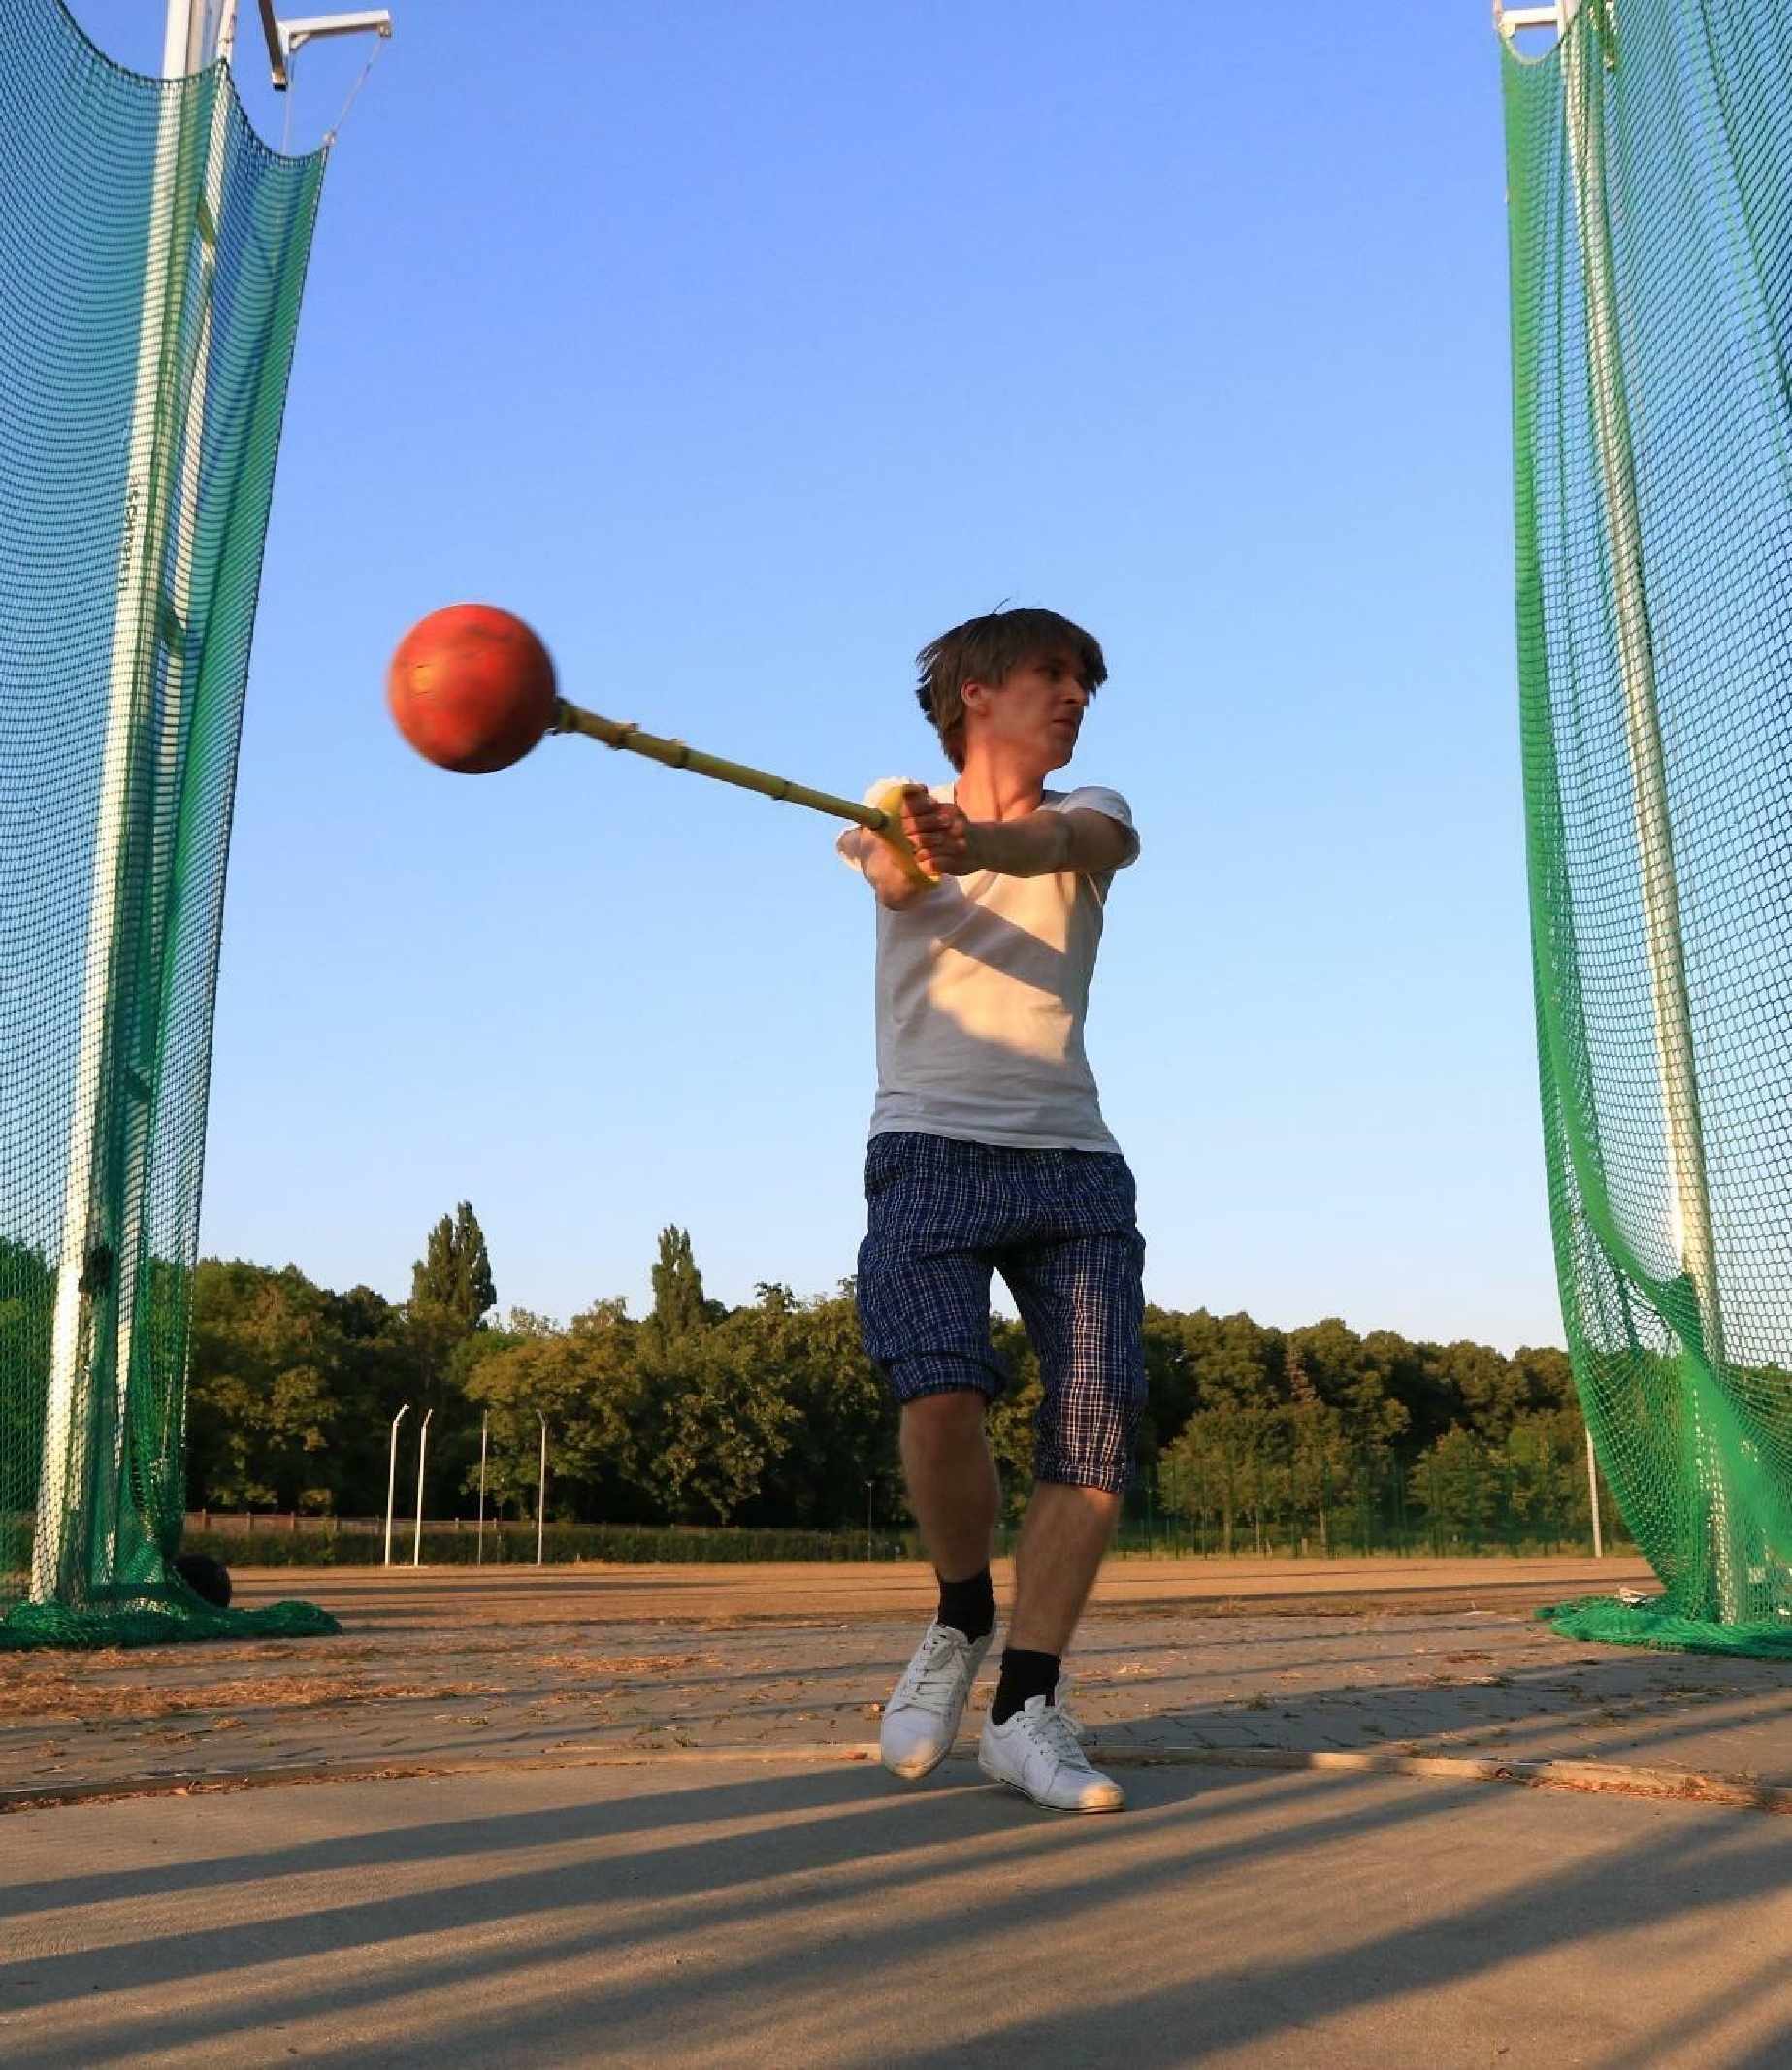
\includegraphics[width=\textwidth]{Hammerwurf.pdf}
\end{minipage}
\medskip
\begin{minipage}{0.5\textwidth}
\begin{flushright}
\small
\emph{Die K�rper w�ren nicht sch�n, \\
wenn sie sich nicht bewegten.\\}
\medskip
Johannes Kepler (1571--1630)\\
\medskip
\emph{Bicycling has done more for the emancipation\\
of women than anything else in the world.}
\medskip 
Susan B. Anthony (1820-1906)
\medskip
\medskip
\emph{Der Sport ist ein sehr vern�nftiger Versuch\\ 
des modernen Zivilisationsmenschen, \\
sich die Strapaze k�nstlich zu verschaffen.\\}
\medskip
Peter Bamm (1879--1975)\\
\medskip
\medskip
\emph{No sports.\\}
\medskip
Sir Winston Churchill (1874--1965)
\normalsize
\end{flushright}
\end{minipage}

\section*{Zusammenfassung des Inhaltes von Kapitel 6 aus Band III -- Sportphysik}\label{kap:spo_zusammenfassung}

Kaum ein Bereich wie der Sport wird von der Physik durchdrungen und das in mehrfacher Hinsicht. 
%\cite{Mathelitsch2015}


\gls{NBA}
%\input{edyn/edyn_zusammenfassung}
%\input{edyn/srt_zusammenfassung}

%% Ende Zusammenfassung

\setcounter{chapter}{8}
\newpage 
\phantomsection
\addcontentsline{toc}{part}{Band V - Optik}
\thispagestyle{empty}
  \begin{flushright}
    \LARGE
    \textbf{Band V \\ \bigskip Optik\\}
  \end{flushright}
  \vspace*{\fill}

%% Achtung diese Zeile auch in optxxx/optxxAB aktivieren 
\addtocontents{toc}{\protect\setcounter{tocdepth}{3}}% alles zeigen bei WorkBook

%%%%%%%%%%%%%%%%%%%%%%%%%%%%%%%%%%%%%%%%%%%%%%%%

\newpage

\include{optbasAB}

%\documentclass[makeidx,envcountchap,graybox,deutsch,ngerman,sectrefs]{svmono}
%\documentclass[envcountchap,graybox,deutsch,sectrefs]{svmono}
%%%%% eigene tempor�re Abk�rzungsliste, f�r die Zeit, bis einheitliche Schreibungen bestehen
\usepackage{tempshort}
%%  Von Springer empfohlene Pakete %% 
%%\documentclass[envcountsect,graybox,deutsch,sectrefs]{svmono}
\usepackage{chapterbib}
\usepackage{type1cm}
\usepackage[ansinew]{inputenc}
\usepackage{babel}
\usepackage[pdftex]{graphicx} %PDF-Vektorgrafiken einbinden
\usepackage{newtxtext} %Typischer Springer-Font
\usepackage{newtxmath}
\usepackage{multicol}
\usepackage[bottom]{footmisc} %Platziert alle Fu�noten unten  
\usepackage[nobreak]{cite}
%\usepackage{biblatex}
\usepackage{cancel}
\usepackage[absolute]{textpos}
\usepackage{graphicx}
\usepackage{pdfpages}

%\usepackage{floatrow}
%\usepackage{mwe}
\usepackage[figuresright]{rotating}
\usepackage{bigints}
\let\laplace\relax  % Vermeidung der Fehlermeldung "\laplace already defined."
\usepackage{trfsigns}
\usepackage{amsmath}
\usepackage{tabulary}
\usepackage{tabularx}

%%  Eigene Pakete %%
\usepackage{adjustbox}
\usepackage{wasysym}
\usepackage{gensymb}
\usepackage{float}
\usepackage{caption}
\usepackage[left=5cm,right=4cm,top=3cm,bottom=4cm,includeheadfoot]{geometry}

%\usepackage{wasysym}
%\usepackage{bigints}
%\usepackage{esint}
%\usepackage{relsize,exscale}

\usepackage{mathtools}   % Vermeidung der Fehlermeldung "Undefined control sequence \coloneqq."


% header and footer
\usepackage{fancyhdr}
\pagestyle{fancy}
\fancyhead[LE,RO]\thepage
\renewcommand{\sectionmark}[1]{\markright{\thesection.\ #1}}
%\fancyhead[LO]{\nouppercase\leftmark}
%\fancyhead[RE]{\nouppercase\rightmark}
\fancyhead[LO]{\nouppercase\rightmark}
\fancyhead[RE]{\nouppercase\leftmark}
\fancyfoot{}
% svmono hat offenbar irgendwas merkw�rdig definiert, darum mu� hier verbreitert werden
%\addtolength\headwidth{25pt}
\setlength{\headheight}{25pt}

%% Units
\usepackage{siunitx}
\sisetup{
  locale = US,
  per-mode = reciprocal, %symbol, % | reciprocal | fraction | ?
  exponent-product = \cdot,
  separate-uncertainty,
  %exponent-to-prefix,
  %prefixes-as-symbols = false,
  %list-units = brackets,% | single | repeat
  %range-units = brackets,% | single | repeat
  %multi-part-units = brackets,% | single | repeat
}
\usepackage{chngcntr}
\usepackage{booktabs}
\usepackage{slashed}
\usepackage{listings}
\usepackage{color} %red, green, blue, yellow, cyan, magenta, black, white
%\usepackage{color} %Einfache Farbendefinition -> von Graybox-Option ben�tigt
\usepackage{multirow}
\usepackage{longtable} %Tabellen �ber mehrere Seiten hinweg
\usepackage{framed} % von Graybox-Option ben�tigt
\usepackage[shortlabels]{enumitem} %Erweiterte Aufz�hloptionen
\usepackage{array}
\usepackage[xindy]{imakeidx} %Wortindex und Personenindex erstellen

\usepackage[hyphens]{url}
%\usepackage[breaklinks,colorlinks=true,linkcolor=black,urlcolor=blue,citecolor=black,filecolor=green,hyperfootnotes=false]{hyperref}
\usepackage[                                    %Hyperref erstellt ein Bookmark/Lesezeichen im PDF. siehe https://www.namsu.de/Extra/pakete/Hyperref.html
bookmarksopen=true,															%Das Lesezeichen ist ge�ffnet beim �ffnen der PDF.
bookmarksnumbered=true,                         %Zahlen werden im Bookmark angezeigt.   
plainpages=false,
pdfpagelabels,
colorlinks=true,                                %Links werden farbig dargestellt.
linkcolor=black, citecolor=black, urlcolor=cyan %Farben definieren.
]{hyperref}                                     %Sollte als letztes eingebunden werden, da es sehr viele Verweise und �nderungen erzeugt. Das Packet ist sehr stark, aber auch umfangreich ist. 

%\usepackage[breaklinks,colorlinks=true,linkcolor=black,urlcolor=blue,citecolor=black,filecolor=green,hyperfootnotes=false]{hyperref}
%\usepackage[breaklinks,colorlinks=true,linkcolor=black,urlcolor=blue,citecolor=black,filecolor=green,hyperfootnotes=false
            %pdftex,
            %pdfauthor={Kaschke, Cartarius},
            %pdftitle={Finger�bungen der Physik}
            %pdfsubject={Ein Repetitorium und �bungsbuch zu im Studium wenig behandelten Kapiteln der Physik mit ausf�hrlich behandelten Problemen und MATLAB-Programmen},
            %pdfkeywords={Physik, Mechanik}
            %]{hyperref}
\pdfminorversion=5

\usepackage{hypcap}
\usepackage[record,section=section,stylemods={mcols},automake]{glossaries-extra}
\usepackage{glossary-longextra}
%\usepackage{glossary-bookindex}
%\makeindex
\setglossarystyle{long-name-sym-desc-loc}
\setabbreviationstyle[acronym]{long-short}

\definecolor{killA}{rgb}{.7,.3,.3}
\newcommand\killA[1]{\bgroup\color{killA}{\cancel{#1}}\egroup}
\newcommand\killB[1]{\bgroup\color{cyan!30!black}{\cancel{#1}}\egroup}

% typographisch korrekte Abk�rzungen (needs to be loaded after hyperref)
\usepackage{abbrev}
\newglossary*{bew}{Glossar}
\newglossary*{hm}{Glossar}
\newglossary*{adyn}{Glossar}
\newglossary*{kontmech}{Glossar}
\newglossary*{aero}{Glossar}
\newglossary*{edyn}{Glossar}
\newglossary*{spo}{Glossar}
\newglossary*{optbas}{Glossar}
\newglossary*{optger}{Glossar}
\newglossary*{optatm}{Glossar}
\newglossary*{optspez}{Glossar}
\GlsXtrLoadResources[src={bew/gloss},type=bew]
\GlsXtrLoadResources[src={hm/gloss},type=hm]
\GlsXtrLoadResources[src={adyn/gloss},type=adyn]
\GlsXtrLoadResources[src={kontmech/gloss},type=kontmech]
\GlsXtrLoadResources[src={aero/gloss},type=aero]
\GlsXtrLoadResources[src={spo/gloss},type=spo]
\GlsXtrLoadResources[src={edyn/gloss},type=edyn]
\GlsXtrLoadResources[src={optbas/gloss},type=optbas]
\GlsXtrLoadResources[src={optger/gloss},type=optger]
\GlsXtrLoadResources[src={optatm/gloss},type=optatm]
\GlsXtrLoadResources[src={optspez/gloss},type=optspez]
\glssetcategoryattribute{bew}{indexname}{true}
%\renewcommand\index\newterm
%\newcolumntype{g}[1]{>{\RaggedRight\hspace{0pt}}p{#1}}
%\renewcommand\glslongextraNameAlign{g}
\renewcommand\glslongextraLocationAlign{@{\ ~\ }>{\raggedright}p{\glspagelistwidth}}
\definecolor{gls}{rgb}{.4,.4,.5}
\renewcommand*{\glstextformat}[1]{\textcolor{gls}{#1}}

%Absatzregeln
\clubpenalty = 30000 %Keine einzelnen Absatzzeilen
\widowpenalty = 30000
\setlength{\parindent}{0em} 
\newcolumntype{L}[1]{>{\raggedright\arraybackslash}p{#1}}
\newcolumntype{C}[1]{>{\centering\arraybackslash}p{#1}}
\newcolumntype{R}[1]{>{\raggedleft\arraybackslash}p{#1}}

\usepackage{xstring}

\newcommand\mfile[2]{%
\saveexpandmode\noexpandarg
\StrSubstitute{#2}{_}{\_}[\tmpname]
\restoreexpandmode
\href{MatlabDateien/\chapname/#1\tmpname}{\tmpname}}

%%% Hyperlinks zu MATLAB Dateien
%\newcommand\mlref[1]{\mfile{}{#1}}
%\newcommand\mlinclref[1]{\mfile{IncludeFolder/}{#1}}
%\newcommand\mldataref[1]{\mfile{Data/}{#1}}

%%% .. f�r ein Verzeichnis hoch
%%% . f�r aktuelle Verzeichnis
%% lokal: MatlabDateien/bew
%\newcommand\mlbewref[1]{\href{MatlabDateien/bew/#1}{#1}}
%% git: https://github.com/sn-code-inside/fingeruebungen-physik/tree/main/bew

\newcommand{\mlrefwithindex}[2]{%
  \index[mfiles]{#2}%   <-- Eintrag im M-File-Index mit aktueller Seitenzahl
  \href{https://github.com/sn-code-inside/fingeruebungen-physik/tree/main/#1/#2}{#2}%
}


%\newcommand\mlbewref[1]{\href{https://github.com/sn-code-inside/fingeruebungen-physik/tree/main/bew/#1}{#1}}
%\newcommand\mlbewdref[1]{\href{https://github.com/sn-code-inside/fingeruebungen-physik/tree/main/bew/Data/#1}{#1}}
%\newcommand\mlbewiref[1]{\href{https://github.com/sn-code-inside/fingeruebungen-physik/tree/main/bew/IncludeFolder/#1}{#1}}
%\newcommand\mlkontmechref[1]{\href{https://github.com/sn-code-inside/fingeruebungen-physik/tree/main/kontmech/#1}{#1}}
%\newcommand\mlkontmechdref[1]{\href{https://github.com/sn-code-inside/fingeruebungen-physik/tree/main/kontmech/Data/#1}{#1}}
%\newcommand\mlkontmechiref[1]{\href{https://github.com/sn-code-inside/fingeruebungen-physik/tree/main/kontmech/IncludeFolder/#1}{#1}}
%\newcommand\mlhmref[1]{\href{https://github.com/sn-code-inside/fingeruebungen-physik/tree/main/hm/#1}{#1}}
%\newcommand\mlhmdref[1]{\href{https://github.com/sn-code-inside/fingeruebungen-physik/tree/main/hm/Data/#1}{#1}}
%\newcommand\mlhmiref[1]{\href{https://github.com/sn-code-inside/fingeruebungen-physik/tree/main/hm/IncludeFolder/#1}{#1}}
%\newcommand\mladynref[1]{\href{https://github.com/sn-code-inside/fingeruebungen-physik/tree/main/adyn/#1}{#1}}
%\newcommand\mladyndref[1]{\href{https://github.com/sn-code-inside/fingeruebungen-physik/tree/main/adyn/Data/#1}{#1}}
%\newcommand\mladyniref[1]{\href{https://github.com/sn-code-inside/fingeruebungen-physik/tree/main/adyn/IncludeFolder/#1}{#1}}
%\newcommand\mledynref[1]{\href{https://github.com/sn-code-inside/fingeruebungen-physik/tree/main/edyn/#1}{#1}}
%\newcommand\mledyndref[1]{\href{https://github.com/sn-code-inside/fingeruebungen-physik/tree/main/edyn/Data/#1}{#1}}
%\newcommand\mledyniref[1]{\href{https://github.com/sn-code-inside/fingeruebungen-physik/tree/main/edyn/IncludeFolder/#1}{#1}}
%\newcommand\mloptbasref[1]{\href{https://github.com/sn-code-inside/fingeruebungen-physik/tree/main/optbas/#1}{#1}}
%\newcommand\mloptbasdref[1]{\href{https://github.com/sn-code-inside/fingeruebungen-physik/tree/main/optbas/Data/#1}{#1}}
%\newcommand\mloptbasiref[1]{\href{https://github.com/sn-code-inside/fingeruebungen-physik/tree/main/optbas/IncludeFolder/#1}{#1}}
%\newcommand\mloptspezref[1]{\href{https://github.com/sn-code-inside/fingeruebungen-physik/tree/main/optspez/#1}{#1}}
%\newcommand\mloptspezdref[1]{\href{https://github.com/sn-code-inside/fingeruebungen-physik/tree/main/optspez/Data/#1}{#1}}
%\newcommand\mloptspeziref[1]{\href{https://github.com/sn-code-inside/fingeruebungen-physik/tree/main/optspez/IncludeFolder/#1}{#1}}

\newcommand\mlbewref[1]{\mlrefwithindex{bew}{#1}}
\newcommand\mlbewdref[1]{\mlrefwithindex{bew/Data}{#1}}
\newcommand\mlbewiref[1]{\mlrefwithindex{bew/Include}{#1}}
\newcommand\mlkontmechref[1]{\mlrefwithindex{kontmech}{#1}}
\newcommand\mlkontmechdref[1]{\mlrefwithindex{kontmech/Data}{#1}}
\newcommand\mlkontmechiref[1]{\mlrefwithindex{kontmech/Include}{#1}}
\newcommand\mlhmref[1]{\mlrefwithindex{hm}{#1}}
\newcommand\mlhmdref[1]{\mlrefwithindex{hm/Data}{#1}}
\newcommand\mlhmiref[1]{\mlrefwithindex{hm/Include}{#1}}
\newcommand\mladynref[1]{\mlrefwithindex{adyn}{#1}}
\newcommand\mladyndref[1]{\mlrefwithindex{adyn/Data}{#1}}
\newcommand\mladyniref[1]{\mlrefwithindex{adyn/Index}{#1}}
\newcommand\mledynref[1]{\mlrefwithindex{edyn}{#1}}
\newcommand\mledyndref[1]{\mlrefwithindex{edyn/Data}{#1}}
\newcommand\mledyniref[1]{\mlrefwithindex{edyn/Index}{#1}}
\newcommand\mloptbasref[1]{\mlrefwithindex{optbas}{#1}}
\newcommand\mloptbasdref[1]{\mlrefwithindex{optbas/Data}{#1}}
\newcommand\mloptbasiref[1]{\mlrefwithindex{optbas/Include}{#1}}
\newcommand\mloptspezref[1]{\mlrefwithindex{optspez}{#1}}
\newcommand\mloptspezdref[1]{\mlrefwithindex{optspez/Data}{#1}}
\newcommand\mloptspeziref[1]{\mlrefwithindex{optspez/Include}{#1}}
\newcommand\mloptgerref[1]{\mlrefwithindex{optger}{#1}}
\newcommand\mloptgerdref[1]{\mlrefwithindex{optger/Data}{#1}}
\newcommand\mloptgeriref[1]{\mlrefwithindex{optger/Include}{#1}}
\newcommand\mloptatmref[1]{\mlrefwithindex{optatm}{#1}}
\newcommand\mloptatmdref[1]{\mlrefwithindex{optatm/Data}{#1}}
\newcommand\mloptatmiref[1]{\mlrefwithindex{optatm/Include}{#1}}



\newcommand\mlcmd[1]{\textcolor{cyan}{\texttt{#1}}}

%Grafikregeln
\graphicspath{{hm/graphs/}
	                    	{bew/graphs/}
     						{kontmech/graphs/}
							{hm/graphs/}
							{adyn/graphs/}
							{edyn/graphs/}
							{kontmech/graphs/}
							{spo/graphs/}
							{optbas/graphs/}
							{optger/graphs/}
							{optatm/graphs/}
							{solman/graphs/}
                                                        {aero/graphs}}
\DeclareGraphicsExtensions{.pdf, .png, .jpg, .jpeg}
\def\figname{Abb}
\newcommand\figref[1]{\figname.\ \ref{abb:#1}}
\usepackage[labelfont=bf]{caption}

\usepackage{tocloft}
\usepackage{etoc}
\setlength\cftfignumwidth{30pt}

% Flatterrand links
\cftsetindents{chapter}{0em}{4em}
\cftsetindents{section}{1.5em}{4em}
\cftsetindents{subsection}{3.8em}{4em}

% flacher Rand links
%\cftsetindents{chapter}{0em}{4em}
%\cftsetindents{section}{0em}{4em}
%\cftsetindents{subsection}{0em}{4em}

\newcommand\partitle[1]{
\addcontentsline{toc}{part}{#1}
\begin{titlepage}
  %\vskip 60%\p@
  \begin{center}
    {\LARGE Finger�bungen der Physik -- #1 \par}
    \vskip 3em%
    {\large Michael Kaschke und Holger Cartarius\par}
  \end{center}
\end{titlepage}
}

%\newcommand\mlref[1]{\href{\chapname/matlab/#1}{#1}}
%\newcommand\mlinclref[1]{\href{\chapname/matlab/IncludeFolder/#1}{\color{cyan}{#1}}}

%Neue Kommandos
\newcommand{\lk}{\left(}        %gro�e runde Klammer (links)
\newcommand{\rk}{\right )}      %gro�e runde Klammer (rechts)
\newcommand{\lgk}{\left \{}     %gro�e geschweifte Klammer (links)
\newcommand{\rgk}{\right \}}    %gro�e geschweifte Klammer (rechts)
\newcommand{\lek}{\left [}      %gro�e eckige Klammer (links)
\newcommand{\rek}{\right ]}     %gro�e eckige Klammer (rechts)
\newcommand{\anf}[1]{\glqq#1\grqq}    %Deutsche Anf�hrungszeichen: \anf{}
\newcommand{\defined}{:=}				%Definition
\newcommand{\curl}{\text{\textbf{rot}}\,}	%Rotation-Operator curl()
\newcommand{\ket}[1]{|#1\rangle}		%Quantenmechanischer Zustand
\newcommand{\curvelintri}{\,\overset{\blacktriangle}{\smallfrown}}
\newcommand{\straighttri}{\blacktriangle}
\newcommand{\UT}{\text{UT}}
\newcommand{\UTC}{\text{UTC}}
\newcommand{\JD}{\text{JD}}
\newcommand{\JDE}{\text{JDE}}
\newcommand{\MJD}{\text{MJD}}
\newcommand{\TDT}{\text{TDT}}
\newcommand{\TT}{\text{TT}}
\newcommand{\NVS}{\text{Navier-Stokes-Gleichungen}}
\newcommand{\MWG}{\text{Maxwell-Gleichungen}}
\newcommand{\EMW}{\text{Elektromagnetische Wellen}}
\newcommand{\eMW}{\text{elektromagnetischen Wellen}}
\newcommand{\RT}{\text{Relativit�tstheorie~}}
\newcommand{\au}{\mathrm{AE}}
\newcommand{\ET}{\text{ET}}
\newcommand{\TAI}{\text{TAI}}
\newcommand{\GMST}{\text{GMST}}
\newcommand{\LMST}{\text{LMST}}
\newcommand{\MESZ}{\text{MESZ}}
\newcommand{\KOS}{\text{Koordinatensystem }}
\newcommand{\DGL}{\text{Differentialgleichung }}
\newcommand{\NA}{\text{NA}}
\newcommand{\uA}{\text{u}}  %atomare Masseneinheit
\newcommand{\MOZ}{\text{MOZ}}
\newcommand{\grad}{\text{\textbf{grad}}\,}	%Gradient-Operator grad()
\newcommand{\uproman}[1]{\mathrm{\uppercase\expandafter{\romannumeral#1}}}
\newcommand{\lowroman}[1]{\romannumeral#1\relax}

\newcommand\todo[1]{\textcolor{red}{TODO: #1}}

\renewcommand{\=}[1]{\stackrel{\text{#1}}{=}}  %Schrift �ber Gleich-Zeichen
\renewcommand{\d}{\partial}
\newcommand{\lra}{\Leftrightarrow}  %�quivalenz-Pfeile
\newcommand{\abs}[1]{\left\vert#1\right\vert}     %Betragsklammern
\renewcommand{\Re}{\mathrm{Re}}                          %Realteil
\renewcommand{\Im}{\mathrm{Im}}                          %Imagin�rteil
\renewcommand{\im}{\mathrm{i}}                         %Imagin�re Einheit
\renewcommand{\epsilon}{\varepsilon} 
\newcommand{\keff}{k_\text{eff}}
\newcommand{\con}{\text{const}}
\newcommand{\conv}{\vec{const}}
\newcommand{\PL}{\mathcal{P}_}
\newcommand{\artanh}{\mathrm{artanh}}
% QED-Symbol im text- bzw. Mathemodus
\newcommand{\textqed}{\hfill ~ $\square$}
\newcommand{\mmqed}{\tag*{$\square$}}

\newcommand{\fa}{(\textbf{a}) }
\newcommand{\fb}{(\textbf{b}) }
\newcommand{\fc}{(\textbf{c}) }
\newcommand{\fd}{(\textbf{d}) }
\newcommand{\fe}{(\textbf{e}) }
\newcommand{\ff}{(\textbf{f}) }

\newcommand{\iF}{im Folgenden~}
\newcommand{\iA}{im Allgemeinen~}


\DeclareMathOperator\divv{div}
\DeclareMathOperator\res{Res}
\DeclareMathOperator{\sech}{sech}
\DeclareMathOperator\sgn{sgn}

% f�r Appendix - MATLAB Referenz
\newcommand{\rotv}{\vec{rot}\,}
\newcommand{\gradv}{\vec{grad}\,}
\newcommand{\nablav}{\vec{\nabla}\,}

\newcommand{\ceil}{\mathrm{ceil}}
\newcommand{\sinc}{\mathrm{sinc}}
\newcommand{\diag}{\mathrm{diag}}
\newcommand{\sign}{\mathrm{sign}}
\newcommand{\length}{\mathrm{length}}
\newcommand{\sort}{\mathrm{sort}}
\newcommand{\summ}{\mathrm{sum}}
\newcommand{\asin}{\mathrm{asin}}
\newcommand{\acos}{\mathrm{acos}}
\newcommand{\atan}{\mathrm{atan}}
\newcommand{\prodd}{\mathrm{prod}}
\newcommand{\median}{\mathrm{mediab}}
\newcommand{\mean}{\mathrm{mean}}
\newcommand{\std}{\mathrm{std}}
\newcommand{\eye}{\mathrm{eye}}
\newcommand{\zeros}{\mathrm{zeros}}
\newcommand{\ones}{\mathrm{ones}}
\newcommand{\rand}{\mathrm{rand}}
\newcommand{\inline}{\mathrm{inline}}
\newcommand{\modd}{\mathrm{mod}}
\newcommand{\floor}{\mathrm{floor}}
\newcommand{\round}{\mathrm{round}}
\newcommand{\rem}{\mathrm{rem}}
\newcommand{\sqrtt}{\mathrm{sqrt}}
\newcommand{\triu}{\mathrm{triu}}
\newcommand{\tril}{\mathrm{tril}}
\newcommand{\size}{\mathrm{size}}
\newcommand{\dett}{\mathrm{det}}
\newcommand{\inv}{\mathrm{inv}}
\newcommand{\rank}{\mathrm{rank}}
\newcommand{\rref}{\mathrm{rref}}
\newcommand{\eig}{\mathrm{eig}}
\newcommand{\poly}{\mathrm{poly}}
\newcommand{\lu}{\mathrm{lu}}
\newcommand{\qr}{\mathrm{qr}}
\newcommand{\quaddd}{\mathrm{quad}}
\newcommand{\fzero}{\mathrm{fzero}}
\newcommand{\roots}{\mathrm{roots}}
\newcommand{\odezd}{\textcolor{mygreen}{\texttt{ode23}}}
\newcommand{\odevf}{\textcolor{mygreen}{\texttt{ode45}}}
\newcommand{\odeeds}{\textcolor{mygreen}{\texttt{ode13s}}}
\newcommand{\odeefs}{\textcolor{mygreen}{\texttt{ode15s}}}
\newcommand{\ddezd}{\textcolor{mygreen}{\texttt{dde23}}}
\newcommand{\onlineZ}{online verf�gbaren Zusatzmaterialien{}}
\newcommand{\MKc}{\url{https://www.fingeruebungen-physik.de}{}}
\newcommand{\linklsg}{\href{https://www.fingeruebungen-physik.de}{\textcolor{blue} {$\rightarrow$ L�sungsteil.}}}
\newcommand{\githubSN}{\url{https://github.com/sn-code-inside/fingeruebungen-physik}{}\,\,}

\newcommand{\FT}{\mathcal{F}} %Fourier-Transformierte

% Aufz�hlung der L�sungen der Teilaufgaben
\newlist{subprobs}{enumerate}{1}
\setlist[subprobs]{
  label= \textbf{\textit{Teilaufgabe}} \textbf{\textit{\arabic*:}} \protect\thissubprob,
  ref=\arabic*, itemsep=\baselineskip, align=left}
\newcommand{\subprob}[1]{
  \def\thissubprob{\textbf{\textit{#1}}}\item ~\vspace{0.2\baselineskip} \newline}

\renewenvironment{example}[1]{
\refstepcounter{example}\par\medskip
\begin{shaded} 
\begin{samepage}
\noindent \textbf{\textit{Beispiel~\theexample: {#1}}}\\ 
\noindent{\color{black} \rule{\textwidth}{0.2 mm}}
\end{samepage}
}{\end{shaded}
\noindent{\color{black} \rule{\textwidth}{0.2 mm}}
} % or snugshade
\definecolor{shadecolor}{gray}{0.95}
\definecolor{mygreen}{RGB}{28,172,0} % color values Red, Green, Blue
\definecolor{mylilas}{RGB}{170,55,241}

\newenvironment{infobox}[1]{
     \begin{shaded} 
     \begin{samepage}
\noindent{\color{black} \rule{\textwidth}{0.2 mm}}
     \end{samepage}
}{\end{shaded}
\noindent{\color{black} \rule{\textwidth}{0.2 mm}}
} 
\definecolor{shadecolor}{gray}{0.95}
\definecolor{mygreen}{RGB}{28,172,0} % color values Red, Green, Blue
\definecolor{mylilas}{RGB}{170,55,241}


\newenvironment{nebenrechnung}[1]{
\begin{shaded} 
\begin{samepage}
\noindent\textbf{Nebenrechnung: \\} 
\noindent{\color{black} \rule{0.1\columnwidth}{0.2mm} \\}
\end{samepage}
}{\end{shaded}
\noindent{\color{black} \rule{0.1\columnwidth}{0.2mm} \\}
} % or snugshade
\definecolor{shadecolor}{gray}{0.95}
\definecolor{mygreen}{RGB}{28,172,0} % color values Red, Green, Blue
\definecolor{mylilas}{RGB}{170,55,241}

\newenvironment{merksatz}[1]{
\begin{shaded} 
\begin{samepage}
\noindent\textbf{Merke:\\} 
\noindent{\color{black} \rule{0.9\columnwidth}{0.2mm} \\ \\}
\end{samepage}
}{\end{shaded}
\noindent{\color{black} \rule{0.9\columnwidth}{0.2mm} \\}
} % or snugshade


\lstset{language=Matlab,%
    %basicstyle=\color{red},
    %basicstyle={\linespread{0.9}\ttfamily},
    basicstyle=\footnotesize\ttfamily,
    breaklines=true,%
    morekeywords={matlab2tikz},
    keywordstyle={\small \color{mygreen}},%
    morekeywords=[2]{1}, keywordstyle=[2]{\small\color{black}},
    identifierstyle={\small \color{black}},%
    stringstyle={\small\color{mylilas}},
    commentstyle={\small\color{mylilas}},%
    showstringspaces=false,%without this there will be a symbol in the places where there is a space
    numbers=left,%
    numberstyle={\tiny \color{black}},% size of the numbers
    numbersep=9pt, % this defines how far the numbers are from the text
    emph=[1]{for,end,else,break, function},emphstyle=[1]\small \color{blue}, %some words to emphasise
    emph=[2]{odeset},emphstyle=[2]\small \color{mygreen}, %some words to emphasise
    %emph=[2]{word1,word2}, emphstyle=[2]{style},    
}

%\bibliographystyle{spphys.bst}

%Trennregeln f�r spezielle Worte
%\hyphenation{Fresnel \matlab �qui-nok-ti-um}

\DeclareSIUnit\erg{erg}
\DeclareSIUnit\cal{cal}
\DeclareSIUnit\celsius{C}
\DeclareSIUnit\m{M}
\DeclareSIUnit\kel{K^{-4}}

%Stichwort- und Personenverzeichnis
\makeindex[title=Stichwortverzeichnis] % Create the default index
\makeindex[name=personen,title=Personenverzeichnis] % Create an index named 'personen'
\newcommand{\indexp}[1]{\index[personen]{#1}}
\makeindex[name=mfiles,title=MATLAB-Skriptverzeichnis,columns=2]

% list of exercises
\newcommand{\loxname}{\Large �bungsverzeichnis}  % einheitliche Gr��e Large
\newlistof[chapter]{prob}{lox}\loxname
\newcommand\uebung[3][]{\label{prob:#2}%
\addcontentsline{lox}{prob}{\protect\numberline{}{\probRef{#2}:~#3#1}}%
\textbf{#1#3}\\[\baselineskip]}
\makeatletter
\renewcommand{\l@prob}{\@dottedtocline{1}{0em}{0em}}
\makeatother

\newcommand\einfach{\uebung[~$\ast$~~]}
\newcommand\mittel{\uebung[~$\ast\,\ast$~~]}
\newcommand\schwierig{\uebung[~$\ast\,\ast\,\ast$~~]}
\newcommand\zusatz{\uebung[~$\ast\,\ast\,\ast\,!$~~]}
%\newcommand\einfach{\uebung[~\textbf{*}~~]}
%\newcommand\mittel{\uebung[~\textbf{*\,*}~~]}
%\newcommand\schwierig{\uebung[~\textbf{*\,*\,*}~]}
%\newcommand\zusatz{\uebung[~\textbf{*\,*\,*\,!}~~]}
\usepackage[atend]{bookmark}
%\BookmarkAtEnd{%
%\bookmarksetup{startatroot}\bookmark[level=0,named=\loxname]{}}

\newcommand\kapitel[1]{Kapitel \ref{kap:#1}}
%\newcommand\kap[1]{Kap.\ \ref{kap:#1}}
\newcommand\kap[1]{Kap. \ref{kap:#1}}

\begin{document}
% customize prob and sol in svmono
\makeatletter
%\counterwithin*{chapter}{part}

\spn@wtheorem{prob}{\bgroup\exercisename\egroup}{\bfseries}{\rmfamily}
\makeatother
\renewenvironment{sol}[1]{\par\addvspace{6pt}\noindent\phantomsection{\textbf{L�sung \ref{#1}}} \ignorespaces}{\par\addvspace{6pt}}
\newcommand\probRef[1]{�bung \ref{prob:#1}}
\renewcommand\probref[1]{\textbf{\probRef{#1}}}
\newcommand\lsgref[1]{L�sung \ref{lsg:#1}}

\newcommand\sbullet[1][.5]{\mathbin{\vcenter{\hbox{\scalebox{#1}{$\bullet$}}}}}

\setcounter{table}{0}


%%%%%%%%%%%%%%%%%%%%%%%%%%%%%%%%%%%%%%%%%%%%%%%%%%%%%%%%%%%%
\chapter{Optische Ger�te}\label{chap:optger}
\def\chapname{optger}
\bibliographystyle{spphys}
\input{optger/optger_motivation}
\clearpage
\input{optger/optger_komponenten}
\clearpage
\input{optger/optger_detektoren}
\clearpage
\input{optger/optger_systeme}
\clearpage
\input{optger/optger_holography}
\clearpage
\input{optger/optger_auge}
\clearpage
%\input{optger/optger_uebungen} 
%\clarpage
%\input{optger/optger_matlabskripts} 
%%\clearpage
%%\input{optger/optger_lsguebungen} 
%\clearpage
%\input{optger/optger_tabellen}
%\renewcommand\glslongextraNameAlign{p{36mm}}
%\renewcommand\glslongextraDescAlign{p{60mm}}
%\clearpage
%\bgroup
%\small
%\printunsrtglossary[type=optger]
%\egroup
%\clearpage
\bibliography{referenzen}
%%%%%%%%%%%%%%%%%%%%%%%%%%%%%%%%%%%%%%%%%%%%%%%%%%%%%%%%%%%%%
%\input{footer.tex}



%\documentclass[makeidx,envcountchap,graybox,deutsch,ngerman,sectrefs]{svmono}
%\documentclass[envcountchap,graybox,deutsch,sectrefs]{svmono}
%%%%% eigene tempor�re Abk�rzungsliste, f�r die Zeit, bis einheitliche Schreibungen bestehen
\usepackage{tempshort}
%%  Von Springer empfohlene Pakete %% 
%%\documentclass[envcountsect,graybox,deutsch,sectrefs]{svmono}
\usepackage{chapterbib}
\usepackage{type1cm}
\usepackage[ansinew]{inputenc}
\usepackage{babel}
\usepackage[pdftex]{graphicx} %PDF-Vektorgrafiken einbinden
\usepackage{newtxtext} %Typischer Springer-Font
\usepackage{newtxmath}
\usepackage{multicol}
\usepackage[bottom]{footmisc} %Platziert alle Fu�noten unten  
\usepackage[nobreak]{cite}
%\usepackage{biblatex}
\usepackage{cancel}
\usepackage[absolute]{textpos}
\usepackage{graphicx}
\usepackage{pdfpages}

%\usepackage{floatrow}
%\usepackage{mwe}
\usepackage[figuresright]{rotating}
\usepackage{bigints}
\let\laplace\relax  % Vermeidung der Fehlermeldung "\laplace already defined."
\usepackage{trfsigns}
\usepackage{amsmath}
\usepackage{tabulary}
\usepackage{tabularx}

%%  Eigene Pakete %%
\usepackage{adjustbox}
\usepackage{wasysym}
\usepackage{gensymb}
\usepackage{float}
\usepackage{caption}
\usepackage[left=5cm,right=4cm,top=3cm,bottom=4cm,includeheadfoot]{geometry}

%\usepackage{wasysym}
%\usepackage{bigints}
%\usepackage{esint}
%\usepackage{relsize,exscale}

\usepackage{mathtools}   % Vermeidung der Fehlermeldung "Undefined control sequence \coloneqq."


% header and footer
\usepackage{fancyhdr}
\pagestyle{fancy}
\fancyhead[LE,RO]\thepage
\renewcommand{\sectionmark}[1]{\markright{\thesection.\ #1}}
%\fancyhead[LO]{\nouppercase\leftmark}
%\fancyhead[RE]{\nouppercase\rightmark}
\fancyhead[LO]{\nouppercase\rightmark}
\fancyhead[RE]{\nouppercase\leftmark}
\fancyfoot{}
% svmono hat offenbar irgendwas merkw�rdig definiert, darum mu� hier verbreitert werden
%\addtolength\headwidth{25pt}
\setlength{\headheight}{25pt}

%% Units
\usepackage{siunitx}
\sisetup{
  locale = US,
  per-mode = reciprocal, %symbol, % | reciprocal | fraction | ?
  exponent-product = \cdot,
  separate-uncertainty,
  %exponent-to-prefix,
  %prefixes-as-symbols = false,
  %list-units = brackets,% | single | repeat
  %range-units = brackets,% | single | repeat
  %multi-part-units = brackets,% | single | repeat
}
\usepackage{chngcntr}
\usepackage{booktabs}
\usepackage{slashed}
\usepackage{listings}
\usepackage{color} %red, green, blue, yellow, cyan, magenta, black, white
%\usepackage{color} %Einfache Farbendefinition -> von Graybox-Option ben�tigt
\usepackage{multirow}
\usepackage{longtable} %Tabellen �ber mehrere Seiten hinweg
\usepackage{framed} % von Graybox-Option ben�tigt
\usepackage[shortlabels]{enumitem} %Erweiterte Aufz�hloptionen
\usepackage{array}
\usepackage[xindy]{imakeidx} %Wortindex und Personenindex erstellen

\usepackage[hyphens]{url}
%\usepackage[breaklinks,colorlinks=true,linkcolor=black,urlcolor=blue,citecolor=black,filecolor=green,hyperfootnotes=false]{hyperref}
\usepackage[                                    %Hyperref erstellt ein Bookmark/Lesezeichen im PDF. siehe https://www.namsu.de/Extra/pakete/Hyperref.html
bookmarksopen=true,															%Das Lesezeichen ist ge�ffnet beim �ffnen der PDF.
bookmarksnumbered=true,                         %Zahlen werden im Bookmark angezeigt.   
plainpages=false,
pdfpagelabels,
colorlinks=true,                                %Links werden farbig dargestellt.
linkcolor=black, citecolor=black, urlcolor=cyan %Farben definieren.
]{hyperref}                                     %Sollte als letztes eingebunden werden, da es sehr viele Verweise und �nderungen erzeugt. Das Packet ist sehr stark, aber auch umfangreich ist. 

%\usepackage[breaklinks,colorlinks=true,linkcolor=black,urlcolor=blue,citecolor=black,filecolor=green,hyperfootnotes=false]{hyperref}
%\usepackage[breaklinks,colorlinks=true,linkcolor=black,urlcolor=blue,citecolor=black,filecolor=green,hyperfootnotes=false
            %pdftex,
            %pdfauthor={Kaschke, Cartarius},
            %pdftitle={Finger�bungen der Physik}
            %pdfsubject={Ein Repetitorium und �bungsbuch zu im Studium wenig behandelten Kapiteln der Physik mit ausf�hrlich behandelten Problemen und MATLAB-Programmen},
            %pdfkeywords={Physik, Mechanik}
            %]{hyperref}
\pdfminorversion=5

\usepackage{hypcap}
\usepackage[record,section=section,stylemods={mcols},automake]{glossaries-extra}
\usepackage{glossary-longextra}
%\usepackage{glossary-bookindex}
%\makeindex
\setglossarystyle{long-name-sym-desc-loc}
\setabbreviationstyle[acronym]{long-short}

\definecolor{killA}{rgb}{.7,.3,.3}
\newcommand\killA[1]{\bgroup\color{killA}{\cancel{#1}}\egroup}
\newcommand\killB[1]{\bgroup\color{cyan!30!black}{\cancel{#1}}\egroup}

% typographisch korrekte Abk�rzungen (needs to be loaded after hyperref)
\usepackage{abbrev}
\newglossary*{bew}{Glossar}
\newglossary*{hm}{Glossar}
\newglossary*{adyn}{Glossar}
\newglossary*{kontmech}{Glossar}
\newglossary*{aero}{Glossar}
\newglossary*{edyn}{Glossar}
\newglossary*{spo}{Glossar}
\newglossary*{optbas}{Glossar}
\newglossary*{optger}{Glossar}
\newglossary*{optatm}{Glossar}
\newglossary*{optspez}{Glossar}
\GlsXtrLoadResources[src={bew/gloss},type=bew]
\GlsXtrLoadResources[src={hm/gloss},type=hm]
\GlsXtrLoadResources[src={adyn/gloss},type=adyn]
\GlsXtrLoadResources[src={kontmech/gloss},type=kontmech]
\GlsXtrLoadResources[src={aero/gloss},type=aero]
\GlsXtrLoadResources[src={spo/gloss},type=spo]
\GlsXtrLoadResources[src={edyn/gloss},type=edyn]
\GlsXtrLoadResources[src={optbas/gloss},type=optbas]
\GlsXtrLoadResources[src={optger/gloss},type=optger]
\GlsXtrLoadResources[src={optatm/gloss},type=optatm]
\GlsXtrLoadResources[src={optspez/gloss},type=optspez]
\glssetcategoryattribute{bew}{indexname}{true}
%\renewcommand\index\newterm
%\newcolumntype{g}[1]{>{\RaggedRight\hspace{0pt}}p{#1}}
%\renewcommand\glslongextraNameAlign{g}
\renewcommand\glslongextraLocationAlign{@{\ ~\ }>{\raggedright}p{\glspagelistwidth}}
\definecolor{gls}{rgb}{.4,.4,.5}
\renewcommand*{\glstextformat}[1]{\textcolor{gls}{#1}}

%Absatzregeln
\clubpenalty = 30000 %Keine einzelnen Absatzzeilen
\widowpenalty = 30000
\setlength{\parindent}{0em} 
\newcolumntype{L}[1]{>{\raggedright\arraybackslash}p{#1}}
\newcolumntype{C}[1]{>{\centering\arraybackslash}p{#1}}
\newcolumntype{R}[1]{>{\raggedleft\arraybackslash}p{#1}}

\usepackage{xstring}

\newcommand\mfile[2]{%
\saveexpandmode\noexpandarg
\StrSubstitute{#2}{_}{\_}[\tmpname]
\restoreexpandmode
\href{MatlabDateien/\chapname/#1\tmpname}{\tmpname}}

%%% Hyperlinks zu MATLAB Dateien
%\newcommand\mlref[1]{\mfile{}{#1}}
%\newcommand\mlinclref[1]{\mfile{IncludeFolder/}{#1}}
%\newcommand\mldataref[1]{\mfile{Data/}{#1}}

%%% .. f�r ein Verzeichnis hoch
%%% . f�r aktuelle Verzeichnis
%% lokal: MatlabDateien/bew
%\newcommand\mlbewref[1]{\href{MatlabDateien/bew/#1}{#1}}
%% git: https://github.com/sn-code-inside/fingeruebungen-physik/tree/main/bew

\newcommand{\mlrefwithindex}[2]{%
  \index[mfiles]{#2}%   <-- Eintrag im M-File-Index mit aktueller Seitenzahl
  \href{https://github.com/sn-code-inside/fingeruebungen-physik/tree/main/#1/#2}{#2}%
}


%\newcommand\mlbewref[1]{\href{https://github.com/sn-code-inside/fingeruebungen-physik/tree/main/bew/#1}{#1}}
%\newcommand\mlbewdref[1]{\href{https://github.com/sn-code-inside/fingeruebungen-physik/tree/main/bew/Data/#1}{#1}}
%\newcommand\mlbewiref[1]{\href{https://github.com/sn-code-inside/fingeruebungen-physik/tree/main/bew/IncludeFolder/#1}{#1}}
%\newcommand\mlkontmechref[1]{\href{https://github.com/sn-code-inside/fingeruebungen-physik/tree/main/kontmech/#1}{#1}}
%\newcommand\mlkontmechdref[1]{\href{https://github.com/sn-code-inside/fingeruebungen-physik/tree/main/kontmech/Data/#1}{#1}}
%\newcommand\mlkontmechiref[1]{\href{https://github.com/sn-code-inside/fingeruebungen-physik/tree/main/kontmech/IncludeFolder/#1}{#1}}
%\newcommand\mlhmref[1]{\href{https://github.com/sn-code-inside/fingeruebungen-physik/tree/main/hm/#1}{#1}}
%\newcommand\mlhmdref[1]{\href{https://github.com/sn-code-inside/fingeruebungen-physik/tree/main/hm/Data/#1}{#1}}
%\newcommand\mlhmiref[1]{\href{https://github.com/sn-code-inside/fingeruebungen-physik/tree/main/hm/IncludeFolder/#1}{#1}}
%\newcommand\mladynref[1]{\href{https://github.com/sn-code-inside/fingeruebungen-physik/tree/main/adyn/#1}{#1}}
%\newcommand\mladyndref[1]{\href{https://github.com/sn-code-inside/fingeruebungen-physik/tree/main/adyn/Data/#1}{#1}}
%\newcommand\mladyniref[1]{\href{https://github.com/sn-code-inside/fingeruebungen-physik/tree/main/adyn/IncludeFolder/#1}{#1}}
%\newcommand\mledynref[1]{\href{https://github.com/sn-code-inside/fingeruebungen-physik/tree/main/edyn/#1}{#1}}
%\newcommand\mledyndref[1]{\href{https://github.com/sn-code-inside/fingeruebungen-physik/tree/main/edyn/Data/#1}{#1}}
%\newcommand\mledyniref[1]{\href{https://github.com/sn-code-inside/fingeruebungen-physik/tree/main/edyn/IncludeFolder/#1}{#1}}
%\newcommand\mloptbasref[1]{\href{https://github.com/sn-code-inside/fingeruebungen-physik/tree/main/optbas/#1}{#1}}
%\newcommand\mloptbasdref[1]{\href{https://github.com/sn-code-inside/fingeruebungen-physik/tree/main/optbas/Data/#1}{#1}}
%\newcommand\mloptbasiref[1]{\href{https://github.com/sn-code-inside/fingeruebungen-physik/tree/main/optbas/IncludeFolder/#1}{#1}}
%\newcommand\mloptspezref[1]{\href{https://github.com/sn-code-inside/fingeruebungen-physik/tree/main/optspez/#1}{#1}}
%\newcommand\mloptspezdref[1]{\href{https://github.com/sn-code-inside/fingeruebungen-physik/tree/main/optspez/Data/#1}{#1}}
%\newcommand\mloptspeziref[1]{\href{https://github.com/sn-code-inside/fingeruebungen-physik/tree/main/optspez/IncludeFolder/#1}{#1}}

\newcommand\mlbewref[1]{\mlrefwithindex{bew}{#1}}
\newcommand\mlbewdref[1]{\mlrefwithindex{bew/Data}{#1}}
\newcommand\mlbewiref[1]{\mlrefwithindex{bew/Include}{#1}}
\newcommand\mlkontmechref[1]{\mlrefwithindex{kontmech}{#1}}
\newcommand\mlkontmechdref[1]{\mlrefwithindex{kontmech/Data}{#1}}
\newcommand\mlkontmechiref[1]{\mlrefwithindex{kontmech/Include}{#1}}
\newcommand\mlhmref[1]{\mlrefwithindex{hm}{#1}}
\newcommand\mlhmdref[1]{\mlrefwithindex{hm/Data}{#1}}
\newcommand\mlhmiref[1]{\mlrefwithindex{hm/Include}{#1}}
\newcommand\mladynref[1]{\mlrefwithindex{adyn}{#1}}
\newcommand\mladyndref[1]{\mlrefwithindex{adyn/Data}{#1}}
\newcommand\mladyniref[1]{\mlrefwithindex{adyn/Index}{#1}}
\newcommand\mledynref[1]{\mlrefwithindex{edyn}{#1}}
\newcommand\mledyndref[1]{\mlrefwithindex{edyn/Data}{#1}}
\newcommand\mledyniref[1]{\mlrefwithindex{edyn/Index}{#1}}
\newcommand\mloptbasref[1]{\mlrefwithindex{optbas}{#1}}
\newcommand\mloptbasdref[1]{\mlrefwithindex{optbas/Data}{#1}}
\newcommand\mloptbasiref[1]{\mlrefwithindex{optbas/Include}{#1}}
\newcommand\mloptspezref[1]{\mlrefwithindex{optspez}{#1}}
\newcommand\mloptspezdref[1]{\mlrefwithindex{optspez/Data}{#1}}
\newcommand\mloptspeziref[1]{\mlrefwithindex{optspez/Include}{#1}}
\newcommand\mloptgerref[1]{\mlrefwithindex{optger}{#1}}
\newcommand\mloptgerdref[1]{\mlrefwithindex{optger/Data}{#1}}
\newcommand\mloptgeriref[1]{\mlrefwithindex{optger/Include}{#1}}
\newcommand\mloptatmref[1]{\mlrefwithindex{optatm}{#1}}
\newcommand\mloptatmdref[1]{\mlrefwithindex{optatm/Data}{#1}}
\newcommand\mloptatmiref[1]{\mlrefwithindex{optatm/Include}{#1}}



\newcommand\mlcmd[1]{\textcolor{cyan}{\texttt{#1}}}

%Grafikregeln
\graphicspath{{hm/graphs/}
	                    	{bew/graphs/}
     						{kontmech/graphs/}
							{hm/graphs/}
							{adyn/graphs/}
							{edyn/graphs/}
							{kontmech/graphs/}
							{spo/graphs/}
							{optbas/graphs/}
							{optger/graphs/}
							{optatm/graphs/}
							{solman/graphs/}
                                                        {aero/graphs}}
\DeclareGraphicsExtensions{.pdf, .png, .jpg, .jpeg}
\def\figname{Abb}
\newcommand\figref[1]{\figname.\ \ref{abb:#1}}
\usepackage[labelfont=bf]{caption}

\usepackage{tocloft}
\usepackage{etoc}
\setlength\cftfignumwidth{30pt}

% Flatterrand links
\cftsetindents{chapter}{0em}{4em}
\cftsetindents{section}{1.5em}{4em}
\cftsetindents{subsection}{3.8em}{4em}

% flacher Rand links
%\cftsetindents{chapter}{0em}{4em}
%\cftsetindents{section}{0em}{4em}
%\cftsetindents{subsection}{0em}{4em}

\newcommand\partitle[1]{
\addcontentsline{toc}{part}{#1}
\begin{titlepage}
  %\vskip 60%\p@
  \begin{center}
    {\LARGE Finger�bungen der Physik -- #1 \par}
    \vskip 3em%
    {\large Michael Kaschke und Holger Cartarius\par}
  \end{center}
\end{titlepage}
}

%\newcommand\mlref[1]{\href{\chapname/matlab/#1}{#1}}
%\newcommand\mlinclref[1]{\href{\chapname/matlab/IncludeFolder/#1}{\color{cyan}{#1}}}

%Neue Kommandos
\newcommand{\lk}{\left(}        %gro�e runde Klammer (links)
\newcommand{\rk}{\right )}      %gro�e runde Klammer (rechts)
\newcommand{\lgk}{\left \{}     %gro�e geschweifte Klammer (links)
\newcommand{\rgk}{\right \}}    %gro�e geschweifte Klammer (rechts)
\newcommand{\lek}{\left [}      %gro�e eckige Klammer (links)
\newcommand{\rek}{\right ]}     %gro�e eckige Klammer (rechts)
\newcommand{\anf}[1]{\glqq#1\grqq}    %Deutsche Anf�hrungszeichen: \anf{}
\newcommand{\defined}{:=}				%Definition
\newcommand{\curl}{\text{\textbf{rot}}\,}	%Rotation-Operator curl()
\newcommand{\ket}[1]{|#1\rangle}		%Quantenmechanischer Zustand
\newcommand{\curvelintri}{\,\overset{\blacktriangle}{\smallfrown}}
\newcommand{\straighttri}{\blacktriangle}
\newcommand{\UT}{\text{UT}}
\newcommand{\UTC}{\text{UTC}}
\newcommand{\JD}{\text{JD}}
\newcommand{\JDE}{\text{JDE}}
\newcommand{\MJD}{\text{MJD}}
\newcommand{\TDT}{\text{TDT}}
\newcommand{\TT}{\text{TT}}
\newcommand{\NVS}{\text{Navier-Stokes-Gleichungen}}
\newcommand{\MWG}{\text{Maxwell-Gleichungen}}
\newcommand{\EMW}{\text{Elektromagnetische Wellen}}
\newcommand{\eMW}{\text{elektromagnetischen Wellen}}
\newcommand{\RT}{\text{Relativit�tstheorie~}}
\newcommand{\au}{\mathrm{AE}}
\newcommand{\ET}{\text{ET}}
\newcommand{\TAI}{\text{TAI}}
\newcommand{\GMST}{\text{GMST}}
\newcommand{\LMST}{\text{LMST}}
\newcommand{\MESZ}{\text{MESZ}}
\newcommand{\KOS}{\text{Koordinatensystem }}
\newcommand{\DGL}{\text{Differentialgleichung }}
\newcommand{\NA}{\text{NA}}
\newcommand{\uA}{\text{u}}  %atomare Masseneinheit
\newcommand{\MOZ}{\text{MOZ}}
\newcommand{\grad}{\text{\textbf{grad}}\,}	%Gradient-Operator grad()
\newcommand{\uproman}[1]{\mathrm{\uppercase\expandafter{\romannumeral#1}}}
\newcommand{\lowroman}[1]{\romannumeral#1\relax}

\newcommand\todo[1]{\textcolor{red}{TODO: #1}}

\renewcommand{\=}[1]{\stackrel{\text{#1}}{=}}  %Schrift �ber Gleich-Zeichen
\renewcommand{\d}{\partial}
\newcommand{\lra}{\Leftrightarrow}  %�quivalenz-Pfeile
\newcommand{\abs}[1]{\left\vert#1\right\vert}     %Betragsklammern
\renewcommand{\Re}{\mathrm{Re}}                          %Realteil
\renewcommand{\Im}{\mathrm{Im}}                          %Imagin�rteil
\renewcommand{\im}{\mathrm{i}}                         %Imagin�re Einheit
\renewcommand{\epsilon}{\varepsilon} 
\newcommand{\keff}{k_\text{eff}}
\newcommand{\con}{\text{const}}
\newcommand{\conv}{\vec{const}}
\newcommand{\PL}{\mathcal{P}_}
\newcommand{\artanh}{\mathrm{artanh}}
% QED-Symbol im text- bzw. Mathemodus
\newcommand{\textqed}{\hfill ~ $\square$}
\newcommand{\mmqed}{\tag*{$\square$}}

\newcommand{\fa}{(\textbf{a}) }
\newcommand{\fb}{(\textbf{b}) }
\newcommand{\fc}{(\textbf{c}) }
\newcommand{\fd}{(\textbf{d}) }
\newcommand{\fe}{(\textbf{e}) }
\newcommand{\ff}{(\textbf{f}) }

\newcommand{\iF}{im Folgenden~}
\newcommand{\iA}{im Allgemeinen~}


\DeclareMathOperator\divv{div}
\DeclareMathOperator\res{Res}
\DeclareMathOperator{\sech}{sech}
\DeclareMathOperator\sgn{sgn}

% f�r Appendix - MATLAB Referenz
\newcommand{\rotv}{\vec{rot}\,}
\newcommand{\gradv}{\vec{grad}\,}
\newcommand{\nablav}{\vec{\nabla}\,}

\newcommand{\ceil}{\mathrm{ceil}}
\newcommand{\sinc}{\mathrm{sinc}}
\newcommand{\diag}{\mathrm{diag}}
\newcommand{\sign}{\mathrm{sign}}
\newcommand{\length}{\mathrm{length}}
\newcommand{\sort}{\mathrm{sort}}
\newcommand{\summ}{\mathrm{sum}}
\newcommand{\asin}{\mathrm{asin}}
\newcommand{\acos}{\mathrm{acos}}
\newcommand{\atan}{\mathrm{atan}}
\newcommand{\prodd}{\mathrm{prod}}
\newcommand{\median}{\mathrm{mediab}}
\newcommand{\mean}{\mathrm{mean}}
\newcommand{\std}{\mathrm{std}}
\newcommand{\eye}{\mathrm{eye}}
\newcommand{\zeros}{\mathrm{zeros}}
\newcommand{\ones}{\mathrm{ones}}
\newcommand{\rand}{\mathrm{rand}}
\newcommand{\inline}{\mathrm{inline}}
\newcommand{\modd}{\mathrm{mod}}
\newcommand{\floor}{\mathrm{floor}}
\newcommand{\round}{\mathrm{round}}
\newcommand{\rem}{\mathrm{rem}}
\newcommand{\sqrtt}{\mathrm{sqrt}}
\newcommand{\triu}{\mathrm{triu}}
\newcommand{\tril}{\mathrm{tril}}
\newcommand{\size}{\mathrm{size}}
\newcommand{\dett}{\mathrm{det}}
\newcommand{\inv}{\mathrm{inv}}
\newcommand{\rank}{\mathrm{rank}}
\newcommand{\rref}{\mathrm{rref}}
\newcommand{\eig}{\mathrm{eig}}
\newcommand{\poly}{\mathrm{poly}}
\newcommand{\lu}{\mathrm{lu}}
\newcommand{\qr}{\mathrm{qr}}
\newcommand{\quaddd}{\mathrm{quad}}
\newcommand{\fzero}{\mathrm{fzero}}
\newcommand{\roots}{\mathrm{roots}}
\newcommand{\odezd}{\textcolor{mygreen}{\texttt{ode23}}}
\newcommand{\odevf}{\textcolor{mygreen}{\texttt{ode45}}}
\newcommand{\odeeds}{\textcolor{mygreen}{\texttt{ode13s}}}
\newcommand{\odeefs}{\textcolor{mygreen}{\texttt{ode15s}}}
\newcommand{\ddezd}{\textcolor{mygreen}{\texttt{dde23}}}
\newcommand{\onlineZ}{online verf�gbaren Zusatzmaterialien{}}
\newcommand{\MKc}{\url{https://www.fingeruebungen-physik.de}{}}
\newcommand{\linklsg}{\href{https://www.fingeruebungen-physik.de}{\textcolor{blue} {$\rightarrow$ L�sungsteil.}}}
\newcommand{\githubSN}{\url{https://github.com/sn-code-inside/fingeruebungen-physik}{}\,\,}

\newcommand{\FT}{\mathcal{F}} %Fourier-Transformierte

% Aufz�hlung der L�sungen der Teilaufgaben
\newlist{subprobs}{enumerate}{1}
\setlist[subprobs]{
  label= \textbf{\textit{Teilaufgabe}} \textbf{\textit{\arabic*:}} \protect\thissubprob,
  ref=\arabic*, itemsep=\baselineskip, align=left}
\newcommand{\subprob}[1]{
  \def\thissubprob{\textbf{\textit{#1}}}\item ~\vspace{0.2\baselineskip} \newline}

\renewenvironment{example}[1]{
\refstepcounter{example}\par\medskip
\begin{shaded} 
\begin{samepage}
\noindent \textbf{\textit{Beispiel~\theexample: {#1}}}\\ 
\noindent{\color{black} \rule{\textwidth}{0.2 mm}}
\end{samepage}
}{\end{shaded}
\noindent{\color{black} \rule{\textwidth}{0.2 mm}}
} % or snugshade
\definecolor{shadecolor}{gray}{0.95}
\definecolor{mygreen}{RGB}{28,172,0} % color values Red, Green, Blue
\definecolor{mylilas}{RGB}{170,55,241}

\newenvironment{infobox}[1]{
     \begin{shaded} 
     \begin{samepage}
\noindent{\color{black} \rule{\textwidth}{0.2 mm}}
     \end{samepage}
}{\end{shaded}
\noindent{\color{black} \rule{\textwidth}{0.2 mm}}
} 
\definecolor{shadecolor}{gray}{0.95}
\definecolor{mygreen}{RGB}{28,172,0} % color values Red, Green, Blue
\definecolor{mylilas}{RGB}{170,55,241}


\newenvironment{nebenrechnung}[1]{
\begin{shaded} 
\begin{samepage}
\noindent\textbf{Nebenrechnung: \\} 
\noindent{\color{black} \rule{0.1\columnwidth}{0.2mm} \\}
\end{samepage}
}{\end{shaded}
\noindent{\color{black} \rule{0.1\columnwidth}{0.2mm} \\}
} % or snugshade
\definecolor{shadecolor}{gray}{0.95}
\definecolor{mygreen}{RGB}{28,172,0} % color values Red, Green, Blue
\definecolor{mylilas}{RGB}{170,55,241}

\newenvironment{merksatz}[1]{
\begin{shaded} 
\begin{samepage}
\noindent\textbf{Merke:\\} 
\noindent{\color{black} \rule{0.9\columnwidth}{0.2mm} \\ \\}
\end{samepage}
}{\end{shaded}
\noindent{\color{black} \rule{0.9\columnwidth}{0.2mm} \\}
} % or snugshade


\lstset{language=Matlab,%
    %basicstyle=\color{red},
    %basicstyle={\linespread{0.9}\ttfamily},
    basicstyle=\footnotesize\ttfamily,
    breaklines=true,%
    morekeywords={matlab2tikz},
    keywordstyle={\small \color{mygreen}},%
    morekeywords=[2]{1}, keywordstyle=[2]{\small\color{black}},
    identifierstyle={\small \color{black}},%
    stringstyle={\small\color{mylilas}},
    commentstyle={\small\color{mylilas}},%
    showstringspaces=false,%without this there will be a symbol in the places where there is a space
    numbers=left,%
    numberstyle={\tiny \color{black}},% size of the numbers
    numbersep=9pt, % this defines how far the numbers are from the text
    emph=[1]{for,end,else,break, function},emphstyle=[1]\small \color{blue}, %some words to emphasise
    emph=[2]{odeset},emphstyle=[2]\small \color{mygreen}, %some words to emphasise
    %emph=[2]{word1,word2}, emphstyle=[2]{style},    
}

%\bibliographystyle{spphys.bst}

%Trennregeln f�r spezielle Worte
%\hyphenation{Fresnel \matlab �qui-nok-ti-um}

\DeclareSIUnit\erg{erg}
\DeclareSIUnit\cal{cal}
\DeclareSIUnit\celsius{C}
\DeclareSIUnit\m{M}
\DeclareSIUnit\kel{K^{-4}}

%Stichwort- und Personenverzeichnis
\makeindex[title=Stichwortverzeichnis] % Create the default index
\makeindex[name=personen,title=Personenverzeichnis] % Create an index named 'personen'
\newcommand{\indexp}[1]{\index[personen]{#1}}
\makeindex[name=mfiles,title=MATLAB-Skriptverzeichnis,columns=2]

% list of exercises
\newcommand{\loxname}{\Large �bungsverzeichnis}  % einheitliche Gr��e Large
\newlistof[chapter]{prob}{lox}\loxname
\newcommand\uebung[3][]{\label{prob:#2}%
\addcontentsline{lox}{prob}{\protect\numberline{}{\probRef{#2}:~#3#1}}%
\textbf{#1#3}\\[\baselineskip]}
\makeatletter
\renewcommand{\l@prob}{\@dottedtocline{1}{0em}{0em}}
\makeatother

\newcommand\einfach{\uebung[~$\ast$~~]}
\newcommand\mittel{\uebung[~$\ast\,\ast$~~]}
\newcommand\schwierig{\uebung[~$\ast\,\ast\,\ast$~~]}
\newcommand\zusatz{\uebung[~$\ast\,\ast\,\ast\,!$~~]}
%\newcommand\einfach{\uebung[~\textbf{*}~~]}
%\newcommand\mittel{\uebung[~\textbf{*\,*}~~]}
%\newcommand\schwierig{\uebung[~\textbf{*\,*\,*}~]}
%\newcommand\zusatz{\uebung[~\textbf{*\,*\,*\,!}~~]}
\usepackage[atend]{bookmark}
%\BookmarkAtEnd{%
%\bookmarksetup{startatroot}\bookmark[level=0,named=\loxname]{}}

\newcommand\kapitel[1]{Kapitel \ref{kap:#1}}
%\newcommand\kap[1]{Kap.\ \ref{kap:#1}}
\newcommand\kap[1]{Kap. \ref{kap:#1}}

\begin{document}
% customize prob and sol in svmono
\makeatletter
%\counterwithin*{chapter}{part}

\spn@wtheorem{prob}{\bgroup\exercisename\egroup}{\bfseries}{\rmfamily}
\makeatother
\renewenvironment{sol}[1]{\par\addvspace{6pt}\noindent\phantomsection{\textbf{L�sung \ref{#1}}} \ignorespaces}{\par\addvspace{6pt}}
\newcommand\probRef[1]{�bung \ref{prob:#1}}
\renewcommand\probref[1]{\textbf{\probRef{#1}}}
\newcommand\lsgref[1]{L�sung \ref{lsg:#1}}

\newcommand\sbullet[1][.5]{\mathbin{\vcenter{\hbox{\scalebox{#1}{$\bullet$}}}}}

\setcounter{table}{0}


%%%%%%%%%%%%%%%%%%%%%%%%%%%%%%%%%%%%%%%%%%%%%%%%%%%%%%%%%%%%
\chapter{Optik der Atmosph�rischen Ph�nomene }\label{chap:optatm}
\def\chapname{optatm}
\bibliographystyle{spphys}
\input{optatm/optatm_motivation}
\clearpage
\input{optatm/optatm_komponenten}
\clearpage
\input{optatm/optatm_anwendungen}
%\clearpage
%\input{optatm/optatm_uebungen} 
%\clearpage
%\input{optatm/optatm_matlabskripts} 
%\clearpage
%\input{optatm/optatm_lsguebungen} 
\clearpage
\input{optatm/optatm_propagationEMW}
\clearpage
\input{optatm/optatm_tabellen}
%\clearpage
%\renewcommand\glslongextraNameAlign{p{36mm}}
%\renewcommand\glslongextraDescAlign{p{60mm}}
%\clearpage
%\bgroup
%\small
%\printunsrtglossary[type=optatm]
%\egroup
\clearpage
\bibliography{referenzen}
%%%%%%%%%%%%%%%%%%%%%%%%%%%%%%%%%%%%%%%%%%%%%%%%%%%%%%%%%%%%%
%\input{footer.tex}


%\documentclass[makeidx,envcountchap,graybox,deutsch,ngerman,sectrefs]{svmono}
%\documentclass[envcountchap,graybox,deutsch,sectrefs]{svmono}
%%%%% eigene tempor�re Abk�rzungsliste, f�r die Zeit, bis einheitliche Schreibungen bestehen
\usepackage{tempshort}
%%  Von Springer empfohlene Pakete %% 
%%\documentclass[envcountsect,graybox,deutsch,sectrefs]{svmono}
\usepackage{chapterbib}
\usepackage{type1cm}
\usepackage[ansinew]{inputenc}
\usepackage{babel}
\usepackage[pdftex]{graphicx} %PDF-Vektorgrafiken einbinden
\usepackage{newtxtext} %Typischer Springer-Font
\usepackage{newtxmath}
\usepackage{multicol}
\usepackage[bottom]{footmisc} %Platziert alle Fu�noten unten  
\usepackage[nobreak]{cite}
%\usepackage{biblatex}
\usepackage{cancel}
\usepackage[absolute]{textpos}
\usepackage{graphicx}
\usepackage{pdfpages}

%\usepackage{floatrow}
%\usepackage{mwe}
\usepackage[figuresright]{rotating}
\usepackage{bigints}
\let\laplace\relax  % Vermeidung der Fehlermeldung "\laplace already defined."
\usepackage{trfsigns}
\usepackage{amsmath}
\usepackage{tabulary}
\usepackage{tabularx}

%%  Eigene Pakete %%
\usepackage{adjustbox}
\usepackage{wasysym}
\usepackage{gensymb}
\usepackage{float}
\usepackage{caption}
\usepackage[left=5cm,right=4cm,top=3cm,bottom=4cm,includeheadfoot]{geometry}

%\usepackage{wasysym}
%\usepackage{bigints}
%\usepackage{esint}
%\usepackage{relsize,exscale}

\usepackage{mathtools}   % Vermeidung der Fehlermeldung "Undefined control sequence \coloneqq."


% header and footer
\usepackage{fancyhdr}
\pagestyle{fancy}
\fancyhead[LE,RO]\thepage
\renewcommand{\sectionmark}[1]{\markright{\thesection.\ #1}}
%\fancyhead[LO]{\nouppercase\leftmark}
%\fancyhead[RE]{\nouppercase\rightmark}
\fancyhead[LO]{\nouppercase\rightmark}
\fancyhead[RE]{\nouppercase\leftmark}
\fancyfoot{}
% svmono hat offenbar irgendwas merkw�rdig definiert, darum mu� hier verbreitert werden
%\addtolength\headwidth{25pt}
\setlength{\headheight}{25pt}

%% Units
\usepackage{siunitx}
\sisetup{
  locale = US,
  per-mode = reciprocal, %symbol, % | reciprocal | fraction | ?
  exponent-product = \cdot,
  separate-uncertainty,
  %exponent-to-prefix,
  %prefixes-as-symbols = false,
  %list-units = brackets,% | single | repeat
  %range-units = brackets,% | single | repeat
  %multi-part-units = brackets,% | single | repeat
}
\usepackage{chngcntr}
\usepackage{booktabs}
\usepackage{slashed}
\usepackage{listings}
\usepackage{color} %red, green, blue, yellow, cyan, magenta, black, white
%\usepackage{color} %Einfache Farbendefinition -> von Graybox-Option ben�tigt
\usepackage{multirow}
\usepackage{longtable} %Tabellen �ber mehrere Seiten hinweg
\usepackage{framed} % von Graybox-Option ben�tigt
\usepackage[shortlabels]{enumitem} %Erweiterte Aufz�hloptionen
\usepackage{array}
\usepackage[xindy]{imakeidx} %Wortindex und Personenindex erstellen

\usepackage[hyphens]{url}
%\usepackage[breaklinks,colorlinks=true,linkcolor=black,urlcolor=blue,citecolor=black,filecolor=green,hyperfootnotes=false]{hyperref}
\usepackage[                                    %Hyperref erstellt ein Bookmark/Lesezeichen im PDF. siehe https://www.namsu.de/Extra/pakete/Hyperref.html
bookmarksopen=true,															%Das Lesezeichen ist ge�ffnet beim �ffnen der PDF.
bookmarksnumbered=true,                         %Zahlen werden im Bookmark angezeigt.   
plainpages=false,
pdfpagelabels,
colorlinks=true,                                %Links werden farbig dargestellt.
linkcolor=black, citecolor=black, urlcolor=cyan %Farben definieren.
]{hyperref}                                     %Sollte als letztes eingebunden werden, da es sehr viele Verweise und �nderungen erzeugt. Das Packet ist sehr stark, aber auch umfangreich ist. 

%\usepackage[breaklinks,colorlinks=true,linkcolor=black,urlcolor=blue,citecolor=black,filecolor=green,hyperfootnotes=false]{hyperref}
%\usepackage[breaklinks,colorlinks=true,linkcolor=black,urlcolor=blue,citecolor=black,filecolor=green,hyperfootnotes=false
            %pdftex,
            %pdfauthor={Kaschke, Cartarius},
            %pdftitle={Finger�bungen der Physik}
            %pdfsubject={Ein Repetitorium und �bungsbuch zu im Studium wenig behandelten Kapiteln der Physik mit ausf�hrlich behandelten Problemen und MATLAB-Programmen},
            %pdfkeywords={Physik, Mechanik}
            %]{hyperref}
\pdfminorversion=5

\usepackage{hypcap}
\usepackage[record,section=section,stylemods={mcols},automake]{glossaries-extra}
\usepackage{glossary-longextra}
%\usepackage{glossary-bookindex}
%\makeindex
\setglossarystyle{long-name-sym-desc-loc}
\setabbreviationstyle[acronym]{long-short}

\definecolor{killA}{rgb}{.7,.3,.3}
\newcommand\killA[1]{\bgroup\color{killA}{\cancel{#1}}\egroup}
\newcommand\killB[1]{\bgroup\color{cyan!30!black}{\cancel{#1}}\egroup}

% typographisch korrekte Abk�rzungen (needs to be loaded after hyperref)
\usepackage{abbrev}
\newglossary*{bew}{Glossar}
\newglossary*{hm}{Glossar}
\newglossary*{adyn}{Glossar}
\newglossary*{kontmech}{Glossar}
\newglossary*{aero}{Glossar}
\newglossary*{edyn}{Glossar}
\newglossary*{spo}{Glossar}
\newglossary*{optbas}{Glossar}
\newglossary*{optger}{Glossar}
\newglossary*{optatm}{Glossar}
\newglossary*{optspez}{Glossar}
\GlsXtrLoadResources[src={bew/gloss},type=bew]
\GlsXtrLoadResources[src={hm/gloss},type=hm]
\GlsXtrLoadResources[src={adyn/gloss},type=adyn]
\GlsXtrLoadResources[src={kontmech/gloss},type=kontmech]
\GlsXtrLoadResources[src={aero/gloss},type=aero]
\GlsXtrLoadResources[src={spo/gloss},type=spo]
\GlsXtrLoadResources[src={edyn/gloss},type=edyn]
\GlsXtrLoadResources[src={optbas/gloss},type=optbas]
\GlsXtrLoadResources[src={optger/gloss},type=optger]
\GlsXtrLoadResources[src={optatm/gloss},type=optatm]
\GlsXtrLoadResources[src={optspez/gloss},type=optspez]
\glssetcategoryattribute{bew}{indexname}{true}
%\renewcommand\index\newterm
%\newcolumntype{g}[1]{>{\RaggedRight\hspace{0pt}}p{#1}}
%\renewcommand\glslongextraNameAlign{g}
\renewcommand\glslongextraLocationAlign{@{\ ~\ }>{\raggedright}p{\glspagelistwidth}}
\definecolor{gls}{rgb}{.4,.4,.5}
\renewcommand*{\glstextformat}[1]{\textcolor{gls}{#1}}

%Absatzregeln
\clubpenalty = 30000 %Keine einzelnen Absatzzeilen
\widowpenalty = 30000
\setlength{\parindent}{0em} 
\newcolumntype{L}[1]{>{\raggedright\arraybackslash}p{#1}}
\newcolumntype{C}[1]{>{\centering\arraybackslash}p{#1}}
\newcolumntype{R}[1]{>{\raggedleft\arraybackslash}p{#1}}

\usepackage{xstring}

\newcommand\mfile[2]{%
\saveexpandmode\noexpandarg
\StrSubstitute{#2}{_}{\_}[\tmpname]
\restoreexpandmode
\href{MatlabDateien/\chapname/#1\tmpname}{\tmpname}}

%%% Hyperlinks zu MATLAB Dateien
%\newcommand\mlref[1]{\mfile{}{#1}}
%\newcommand\mlinclref[1]{\mfile{IncludeFolder/}{#1}}
%\newcommand\mldataref[1]{\mfile{Data/}{#1}}

%%% .. f�r ein Verzeichnis hoch
%%% . f�r aktuelle Verzeichnis
%% lokal: MatlabDateien/bew
%\newcommand\mlbewref[1]{\href{MatlabDateien/bew/#1}{#1}}
%% git: https://github.com/sn-code-inside/fingeruebungen-physik/tree/main/bew

\newcommand{\mlrefwithindex}[2]{%
  \index[mfiles]{#2}%   <-- Eintrag im M-File-Index mit aktueller Seitenzahl
  \href{https://github.com/sn-code-inside/fingeruebungen-physik/tree/main/#1/#2}{#2}%
}


%\newcommand\mlbewref[1]{\href{https://github.com/sn-code-inside/fingeruebungen-physik/tree/main/bew/#1}{#1}}
%\newcommand\mlbewdref[1]{\href{https://github.com/sn-code-inside/fingeruebungen-physik/tree/main/bew/Data/#1}{#1}}
%\newcommand\mlbewiref[1]{\href{https://github.com/sn-code-inside/fingeruebungen-physik/tree/main/bew/IncludeFolder/#1}{#1}}
%\newcommand\mlkontmechref[1]{\href{https://github.com/sn-code-inside/fingeruebungen-physik/tree/main/kontmech/#1}{#1}}
%\newcommand\mlkontmechdref[1]{\href{https://github.com/sn-code-inside/fingeruebungen-physik/tree/main/kontmech/Data/#1}{#1}}
%\newcommand\mlkontmechiref[1]{\href{https://github.com/sn-code-inside/fingeruebungen-physik/tree/main/kontmech/IncludeFolder/#1}{#1}}
%\newcommand\mlhmref[1]{\href{https://github.com/sn-code-inside/fingeruebungen-physik/tree/main/hm/#1}{#1}}
%\newcommand\mlhmdref[1]{\href{https://github.com/sn-code-inside/fingeruebungen-physik/tree/main/hm/Data/#1}{#1}}
%\newcommand\mlhmiref[1]{\href{https://github.com/sn-code-inside/fingeruebungen-physik/tree/main/hm/IncludeFolder/#1}{#1}}
%\newcommand\mladynref[1]{\href{https://github.com/sn-code-inside/fingeruebungen-physik/tree/main/adyn/#1}{#1}}
%\newcommand\mladyndref[1]{\href{https://github.com/sn-code-inside/fingeruebungen-physik/tree/main/adyn/Data/#1}{#1}}
%\newcommand\mladyniref[1]{\href{https://github.com/sn-code-inside/fingeruebungen-physik/tree/main/adyn/IncludeFolder/#1}{#1}}
%\newcommand\mledynref[1]{\href{https://github.com/sn-code-inside/fingeruebungen-physik/tree/main/edyn/#1}{#1}}
%\newcommand\mledyndref[1]{\href{https://github.com/sn-code-inside/fingeruebungen-physik/tree/main/edyn/Data/#1}{#1}}
%\newcommand\mledyniref[1]{\href{https://github.com/sn-code-inside/fingeruebungen-physik/tree/main/edyn/IncludeFolder/#1}{#1}}
%\newcommand\mloptbasref[1]{\href{https://github.com/sn-code-inside/fingeruebungen-physik/tree/main/optbas/#1}{#1}}
%\newcommand\mloptbasdref[1]{\href{https://github.com/sn-code-inside/fingeruebungen-physik/tree/main/optbas/Data/#1}{#1}}
%\newcommand\mloptbasiref[1]{\href{https://github.com/sn-code-inside/fingeruebungen-physik/tree/main/optbas/IncludeFolder/#1}{#1}}
%\newcommand\mloptspezref[1]{\href{https://github.com/sn-code-inside/fingeruebungen-physik/tree/main/optspez/#1}{#1}}
%\newcommand\mloptspezdref[1]{\href{https://github.com/sn-code-inside/fingeruebungen-physik/tree/main/optspez/Data/#1}{#1}}
%\newcommand\mloptspeziref[1]{\href{https://github.com/sn-code-inside/fingeruebungen-physik/tree/main/optspez/IncludeFolder/#1}{#1}}

\newcommand\mlbewref[1]{\mlrefwithindex{bew}{#1}}
\newcommand\mlbewdref[1]{\mlrefwithindex{bew/Data}{#1}}
\newcommand\mlbewiref[1]{\mlrefwithindex{bew/Include}{#1}}
\newcommand\mlkontmechref[1]{\mlrefwithindex{kontmech}{#1}}
\newcommand\mlkontmechdref[1]{\mlrefwithindex{kontmech/Data}{#1}}
\newcommand\mlkontmechiref[1]{\mlrefwithindex{kontmech/Include}{#1}}
\newcommand\mlhmref[1]{\mlrefwithindex{hm}{#1}}
\newcommand\mlhmdref[1]{\mlrefwithindex{hm/Data}{#1}}
\newcommand\mlhmiref[1]{\mlrefwithindex{hm/Include}{#1}}
\newcommand\mladynref[1]{\mlrefwithindex{adyn}{#1}}
\newcommand\mladyndref[1]{\mlrefwithindex{adyn/Data}{#1}}
\newcommand\mladyniref[1]{\mlrefwithindex{adyn/Index}{#1}}
\newcommand\mledynref[1]{\mlrefwithindex{edyn}{#1}}
\newcommand\mledyndref[1]{\mlrefwithindex{edyn/Data}{#1}}
\newcommand\mledyniref[1]{\mlrefwithindex{edyn/Index}{#1}}
\newcommand\mloptbasref[1]{\mlrefwithindex{optbas}{#1}}
\newcommand\mloptbasdref[1]{\mlrefwithindex{optbas/Data}{#1}}
\newcommand\mloptbasiref[1]{\mlrefwithindex{optbas/Include}{#1}}
\newcommand\mloptspezref[1]{\mlrefwithindex{optspez}{#1}}
\newcommand\mloptspezdref[1]{\mlrefwithindex{optspez/Data}{#1}}
\newcommand\mloptspeziref[1]{\mlrefwithindex{optspez/Include}{#1}}
\newcommand\mloptgerref[1]{\mlrefwithindex{optger}{#1}}
\newcommand\mloptgerdref[1]{\mlrefwithindex{optger/Data}{#1}}
\newcommand\mloptgeriref[1]{\mlrefwithindex{optger/Include}{#1}}
\newcommand\mloptatmref[1]{\mlrefwithindex{optatm}{#1}}
\newcommand\mloptatmdref[1]{\mlrefwithindex{optatm/Data}{#1}}
\newcommand\mloptatmiref[1]{\mlrefwithindex{optatm/Include}{#1}}



\newcommand\mlcmd[1]{\textcolor{cyan}{\texttt{#1}}}

%Grafikregeln
\graphicspath{{hm/graphs/}
	                    	{bew/graphs/}
     						{kontmech/graphs/}
							{hm/graphs/}
							{adyn/graphs/}
							{edyn/graphs/}
							{kontmech/graphs/}
							{spo/graphs/}
							{optbas/graphs/}
							{optger/graphs/}
							{optatm/graphs/}
							{solman/graphs/}
                                                        {aero/graphs}}
\DeclareGraphicsExtensions{.pdf, .png, .jpg, .jpeg}
\def\figname{Abb}
\newcommand\figref[1]{\figname.\ \ref{abb:#1}}
\usepackage[labelfont=bf]{caption}

\usepackage{tocloft}
\usepackage{etoc}
\setlength\cftfignumwidth{30pt}

% Flatterrand links
\cftsetindents{chapter}{0em}{4em}
\cftsetindents{section}{1.5em}{4em}
\cftsetindents{subsection}{3.8em}{4em}

% flacher Rand links
%\cftsetindents{chapter}{0em}{4em}
%\cftsetindents{section}{0em}{4em}
%\cftsetindents{subsection}{0em}{4em}

\newcommand\partitle[1]{
\addcontentsline{toc}{part}{#1}
\begin{titlepage}
  %\vskip 60%\p@
  \begin{center}
    {\LARGE Finger�bungen der Physik -- #1 \par}
    \vskip 3em%
    {\large Michael Kaschke und Holger Cartarius\par}
  \end{center}
\end{titlepage}
}

%\newcommand\mlref[1]{\href{\chapname/matlab/#1}{#1}}
%\newcommand\mlinclref[1]{\href{\chapname/matlab/IncludeFolder/#1}{\color{cyan}{#1}}}

%Neue Kommandos
\newcommand{\lk}{\left(}        %gro�e runde Klammer (links)
\newcommand{\rk}{\right )}      %gro�e runde Klammer (rechts)
\newcommand{\lgk}{\left \{}     %gro�e geschweifte Klammer (links)
\newcommand{\rgk}{\right \}}    %gro�e geschweifte Klammer (rechts)
\newcommand{\lek}{\left [}      %gro�e eckige Klammer (links)
\newcommand{\rek}{\right ]}     %gro�e eckige Klammer (rechts)
\newcommand{\anf}[1]{\glqq#1\grqq}    %Deutsche Anf�hrungszeichen: \anf{}
\newcommand{\defined}{:=}				%Definition
\newcommand{\curl}{\text{\textbf{rot}}\,}	%Rotation-Operator curl()
\newcommand{\ket}[1]{|#1\rangle}		%Quantenmechanischer Zustand
\newcommand{\curvelintri}{\,\overset{\blacktriangle}{\smallfrown}}
\newcommand{\straighttri}{\blacktriangle}
\newcommand{\UT}{\text{UT}}
\newcommand{\UTC}{\text{UTC}}
\newcommand{\JD}{\text{JD}}
\newcommand{\JDE}{\text{JDE}}
\newcommand{\MJD}{\text{MJD}}
\newcommand{\TDT}{\text{TDT}}
\newcommand{\TT}{\text{TT}}
\newcommand{\NVS}{\text{Navier-Stokes-Gleichungen}}
\newcommand{\MWG}{\text{Maxwell-Gleichungen}}
\newcommand{\EMW}{\text{Elektromagnetische Wellen}}
\newcommand{\eMW}{\text{elektromagnetischen Wellen}}
\newcommand{\RT}{\text{Relativit�tstheorie~}}
\newcommand{\au}{\mathrm{AE}}
\newcommand{\ET}{\text{ET}}
\newcommand{\TAI}{\text{TAI}}
\newcommand{\GMST}{\text{GMST}}
\newcommand{\LMST}{\text{LMST}}
\newcommand{\MESZ}{\text{MESZ}}
\newcommand{\KOS}{\text{Koordinatensystem }}
\newcommand{\DGL}{\text{Differentialgleichung }}
\newcommand{\NA}{\text{NA}}
\newcommand{\uA}{\text{u}}  %atomare Masseneinheit
\newcommand{\MOZ}{\text{MOZ}}
\newcommand{\grad}{\text{\textbf{grad}}\,}	%Gradient-Operator grad()
\newcommand{\uproman}[1]{\mathrm{\uppercase\expandafter{\romannumeral#1}}}
\newcommand{\lowroman}[1]{\romannumeral#1\relax}

\newcommand\todo[1]{\textcolor{red}{TODO: #1}}

\renewcommand{\=}[1]{\stackrel{\text{#1}}{=}}  %Schrift �ber Gleich-Zeichen
\renewcommand{\d}{\partial}
\newcommand{\lra}{\Leftrightarrow}  %�quivalenz-Pfeile
\newcommand{\abs}[1]{\left\vert#1\right\vert}     %Betragsklammern
\renewcommand{\Re}{\mathrm{Re}}                          %Realteil
\renewcommand{\Im}{\mathrm{Im}}                          %Imagin�rteil
\renewcommand{\im}{\mathrm{i}}                         %Imagin�re Einheit
\renewcommand{\epsilon}{\varepsilon} 
\newcommand{\keff}{k_\text{eff}}
\newcommand{\con}{\text{const}}
\newcommand{\conv}{\vec{const}}
\newcommand{\PL}{\mathcal{P}_}
\newcommand{\artanh}{\mathrm{artanh}}
% QED-Symbol im text- bzw. Mathemodus
\newcommand{\textqed}{\hfill ~ $\square$}
\newcommand{\mmqed}{\tag*{$\square$}}

\newcommand{\fa}{(\textbf{a}) }
\newcommand{\fb}{(\textbf{b}) }
\newcommand{\fc}{(\textbf{c}) }
\newcommand{\fd}{(\textbf{d}) }
\newcommand{\fe}{(\textbf{e}) }
\newcommand{\ff}{(\textbf{f}) }

\newcommand{\iF}{im Folgenden~}
\newcommand{\iA}{im Allgemeinen~}


\DeclareMathOperator\divv{div}
\DeclareMathOperator\res{Res}
\DeclareMathOperator{\sech}{sech}
\DeclareMathOperator\sgn{sgn}

% f�r Appendix - MATLAB Referenz
\newcommand{\rotv}{\vec{rot}\,}
\newcommand{\gradv}{\vec{grad}\,}
\newcommand{\nablav}{\vec{\nabla}\,}

\newcommand{\ceil}{\mathrm{ceil}}
\newcommand{\sinc}{\mathrm{sinc}}
\newcommand{\diag}{\mathrm{diag}}
\newcommand{\sign}{\mathrm{sign}}
\newcommand{\length}{\mathrm{length}}
\newcommand{\sort}{\mathrm{sort}}
\newcommand{\summ}{\mathrm{sum}}
\newcommand{\asin}{\mathrm{asin}}
\newcommand{\acos}{\mathrm{acos}}
\newcommand{\atan}{\mathrm{atan}}
\newcommand{\prodd}{\mathrm{prod}}
\newcommand{\median}{\mathrm{mediab}}
\newcommand{\mean}{\mathrm{mean}}
\newcommand{\std}{\mathrm{std}}
\newcommand{\eye}{\mathrm{eye}}
\newcommand{\zeros}{\mathrm{zeros}}
\newcommand{\ones}{\mathrm{ones}}
\newcommand{\rand}{\mathrm{rand}}
\newcommand{\inline}{\mathrm{inline}}
\newcommand{\modd}{\mathrm{mod}}
\newcommand{\floor}{\mathrm{floor}}
\newcommand{\round}{\mathrm{round}}
\newcommand{\rem}{\mathrm{rem}}
\newcommand{\sqrtt}{\mathrm{sqrt}}
\newcommand{\triu}{\mathrm{triu}}
\newcommand{\tril}{\mathrm{tril}}
\newcommand{\size}{\mathrm{size}}
\newcommand{\dett}{\mathrm{det}}
\newcommand{\inv}{\mathrm{inv}}
\newcommand{\rank}{\mathrm{rank}}
\newcommand{\rref}{\mathrm{rref}}
\newcommand{\eig}{\mathrm{eig}}
\newcommand{\poly}{\mathrm{poly}}
\newcommand{\lu}{\mathrm{lu}}
\newcommand{\qr}{\mathrm{qr}}
\newcommand{\quaddd}{\mathrm{quad}}
\newcommand{\fzero}{\mathrm{fzero}}
\newcommand{\roots}{\mathrm{roots}}
\newcommand{\odezd}{\textcolor{mygreen}{\texttt{ode23}}}
\newcommand{\odevf}{\textcolor{mygreen}{\texttt{ode45}}}
\newcommand{\odeeds}{\textcolor{mygreen}{\texttt{ode13s}}}
\newcommand{\odeefs}{\textcolor{mygreen}{\texttt{ode15s}}}
\newcommand{\ddezd}{\textcolor{mygreen}{\texttt{dde23}}}
\newcommand{\onlineZ}{online verf�gbaren Zusatzmaterialien{}}
\newcommand{\MKc}{\url{https://www.fingeruebungen-physik.de}{}}
\newcommand{\linklsg}{\href{https://www.fingeruebungen-physik.de}{\textcolor{blue} {$\rightarrow$ L�sungsteil.}}}
\newcommand{\githubSN}{\url{https://github.com/sn-code-inside/fingeruebungen-physik}{}\,\,}

\newcommand{\FT}{\mathcal{F}} %Fourier-Transformierte

% Aufz�hlung der L�sungen der Teilaufgaben
\newlist{subprobs}{enumerate}{1}
\setlist[subprobs]{
  label= \textbf{\textit{Teilaufgabe}} \textbf{\textit{\arabic*:}} \protect\thissubprob,
  ref=\arabic*, itemsep=\baselineskip, align=left}
\newcommand{\subprob}[1]{
  \def\thissubprob{\textbf{\textit{#1}}}\item ~\vspace{0.2\baselineskip} \newline}

\renewenvironment{example}[1]{
\refstepcounter{example}\par\medskip
\begin{shaded} 
\begin{samepage}
\noindent \textbf{\textit{Beispiel~\theexample: {#1}}}\\ 
\noindent{\color{black} \rule{\textwidth}{0.2 mm}}
\end{samepage}
}{\end{shaded}
\noindent{\color{black} \rule{\textwidth}{0.2 mm}}
} % or snugshade
\definecolor{shadecolor}{gray}{0.95}
\definecolor{mygreen}{RGB}{28,172,0} % color values Red, Green, Blue
\definecolor{mylilas}{RGB}{170,55,241}

\newenvironment{infobox}[1]{
     \begin{shaded} 
     \begin{samepage}
\noindent{\color{black} \rule{\textwidth}{0.2 mm}}
     \end{samepage}
}{\end{shaded}
\noindent{\color{black} \rule{\textwidth}{0.2 mm}}
} 
\definecolor{shadecolor}{gray}{0.95}
\definecolor{mygreen}{RGB}{28,172,0} % color values Red, Green, Blue
\definecolor{mylilas}{RGB}{170,55,241}


\newenvironment{nebenrechnung}[1]{
\begin{shaded} 
\begin{samepage}
\noindent\textbf{Nebenrechnung: \\} 
\noindent{\color{black} \rule{0.1\columnwidth}{0.2mm} \\}
\end{samepage}
}{\end{shaded}
\noindent{\color{black} \rule{0.1\columnwidth}{0.2mm} \\}
} % or snugshade
\definecolor{shadecolor}{gray}{0.95}
\definecolor{mygreen}{RGB}{28,172,0} % color values Red, Green, Blue
\definecolor{mylilas}{RGB}{170,55,241}

\newenvironment{merksatz}[1]{
\begin{shaded} 
\begin{samepage}
\noindent\textbf{Merke:\\} 
\noindent{\color{black} \rule{0.9\columnwidth}{0.2mm} \\ \\}
\end{samepage}
}{\end{shaded}
\noindent{\color{black} \rule{0.9\columnwidth}{0.2mm} \\}
} % or snugshade


\lstset{language=Matlab,%
    %basicstyle=\color{red},
    %basicstyle={\linespread{0.9}\ttfamily},
    basicstyle=\footnotesize\ttfamily,
    breaklines=true,%
    morekeywords={matlab2tikz},
    keywordstyle={\small \color{mygreen}},%
    morekeywords=[2]{1}, keywordstyle=[2]{\small\color{black}},
    identifierstyle={\small \color{black}},%
    stringstyle={\small\color{mylilas}},
    commentstyle={\small\color{mylilas}},%
    showstringspaces=false,%without this there will be a symbol in the places where there is a space
    numbers=left,%
    numberstyle={\tiny \color{black}},% size of the numbers
    numbersep=9pt, % this defines how far the numbers are from the text
    emph=[1]{for,end,else,break, function},emphstyle=[1]\small \color{blue}, %some words to emphasise
    emph=[2]{odeset},emphstyle=[2]\small \color{mygreen}, %some words to emphasise
    %emph=[2]{word1,word2}, emphstyle=[2]{style},    
}

%\bibliographystyle{spphys.bst}

%Trennregeln f�r spezielle Worte
%\hyphenation{Fresnel \matlab �qui-nok-ti-um}

\DeclareSIUnit\erg{erg}
\DeclareSIUnit\cal{cal}
\DeclareSIUnit\celsius{C}
\DeclareSIUnit\m{M}
\DeclareSIUnit\kel{K^{-4}}

%Stichwort- und Personenverzeichnis
\makeindex[title=Stichwortverzeichnis] % Create the default index
\makeindex[name=personen,title=Personenverzeichnis] % Create an index named 'personen'
\newcommand{\indexp}[1]{\index[personen]{#1}}
\makeindex[name=mfiles,title=MATLAB-Skriptverzeichnis,columns=2]

% list of exercises
\newcommand{\loxname}{\Large �bungsverzeichnis}  % einheitliche Gr��e Large
\newlistof[chapter]{prob}{lox}\loxname
\newcommand\uebung[3][]{\label{prob:#2}%
\addcontentsline{lox}{prob}{\protect\numberline{}{\probRef{#2}:~#3#1}}%
\textbf{#1#3}\\[\baselineskip]}
\makeatletter
\renewcommand{\l@prob}{\@dottedtocline{1}{0em}{0em}}
\makeatother

\newcommand\einfach{\uebung[~$\ast$~~]}
\newcommand\mittel{\uebung[~$\ast\,\ast$~~]}
\newcommand\schwierig{\uebung[~$\ast\,\ast\,\ast$~~]}
\newcommand\zusatz{\uebung[~$\ast\,\ast\,\ast\,!$~~]}
%\newcommand\einfach{\uebung[~\textbf{*}~~]}
%\newcommand\mittel{\uebung[~\textbf{*\,*}~~]}
%\newcommand\schwierig{\uebung[~\textbf{*\,*\,*}~]}
%\newcommand\zusatz{\uebung[~\textbf{*\,*\,*\,!}~~]}
\usepackage[atend]{bookmark}
%\BookmarkAtEnd{%
%\bookmarksetup{startatroot}\bookmark[level=0,named=\loxname]{}}

\newcommand\kapitel[1]{Kapitel \ref{kap:#1}}
%\newcommand\kap[1]{Kap.\ \ref{kap:#1}}
\newcommand\kap[1]{Kap. \ref{kap:#1}}

\begin{document}
% customize prob and sol in svmono
\makeatletter
%\counterwithin*{chapter}{part}

\spn@wtheorem{prob}{\bgroup\exercisename\egroup}{\bfseries}{\rmfamily}
\makeatother
\renewenvironment{sol}[1]{\par\addvspace{6pt}\noindent\phantomsection{\textbf{L�sung \ref{#1}}} \ignorespaces}{\par\addvspace{6pt}}
\newcommand\probRef[1]{�bung \ref{prob:#1}}
\renewcommand\probref[1]{\textbf{\probRef{#1}}}
\newcommand\lsgref[1]{L�sung \ref{lsg:#1}}

\newcommand\sbullet[1][.5]{\mathbin{\vcenter{\hbox{\scalebox{#1}{$\bullet$}}}}}

\setcounter{table}{0}



% f�r funktionierende Hyperlinks zwei neue Environments mit eigenen Countern, up. 2024-01-29
\newcounter{partsectionU}
\newcounter{partsectionL}
\newcounter{partsectionA}

\newenvironment{PartU}[1]
 {%
  \cleardoublepage
  \phantomsection
  \setcounter{section}{\value{partsectionU}}%
  \renewcommand{\thesection}{\"U\arabic{section}}%
  \renewcommand{\theHsection}{SU\arabic{section}}%
  \addcontentsline{toc}{part}{#1}%
  \thispagestyle{empty}
  \begin{flushright}
    \LARGE
    \textbf{
  �bungen\\ \bigskip  Band V\\ \bigskip Optik\\}
  \end{flushright}
  \vspace*{\fill}
  \clearpage
 }
 {%
  \setcounter{partsectionU}{\value{section}}%
  \cleardoublepage
}

\newenvironment{PartL}[1]
 {%
  \cleardoublepage
  \phantomsection
  \setcounter{section}{\value{partsectionL}}%
  \renewcommand{\thesection}{L\arabic{section}}%
  \renewcommand{\theHsection}{SL\arabic{section}}%
  \addcontentsline{toc}{part}{#1}%
  \thispagestyle{empty}
  \begin{flushright}
    \LARGE
    \textbf{L�sungsvorschl�ge \\ \bigskip Band V \\ \bigskip Optik\\}
  \end{flushright}
  \vspace*{\fill}
  \clearpage
 }
 {%
  \setcounter{partsectionL}{\value{section}}%
 \cleardoublepage
}

\newenvironment{PartA}[1]
 {%
  \cleardoublepage
  \phantomsection
  \setcounter{section}{\value{partsectionA}}%
  \renewcommand{\thesection}{A\arabic{section}}%
  \renewcommand{\theHsection}{SA\arabic{section}}%
  \addcontentsline{toc}{part}{#1}%
  \thispagestyle{empty}
  \begin{flushright}
    \LARGE
    \textbf{Appendix \\ \bigskip Band V \\ \bigskip Optik\\}
  \end{flushright}
  \vspace*{\fill}
  \clearpage
 }
 {%
  \setcounter{partsectionA}{\value{section}}%
 \cleardoublepage
}


%%%%%%%%%%%%%%%%%%%%%%%%%%%%%%%%%%%%%%%%%%%%%%%%%%%%%%%%%%%%%

\bibliographystyle{spphys}

\makeatletter
\@addtoreset{chapter}{part}
\makeatother
\renewcommand{\thechapter}{�\,\arabic{chapter}}

\addtocontents{toc}{\protect\setcounter{tocdepth}{2}}% alles zeigen

\begin{PartU}{�bungen - Band V Optik}
\setcounter{chapter}{9}
\setcounter{section}{8}
\setcounter{subsection}{0}
\setcounter{figure}{0}
\setcounter{equation}{0}
\setcounter{prob}{0}
\counterwithin{prob}{chapter}
\counterwithin{table}{section}
\setcounter{table}{0}
\newpage
\quad 
\newpage
\input{optbas/optbas_uebungenAB}
\setcounter{chapter}{10}
\setcounter{figure}{0}
\setcounter{equation}{0}
\setcounter{prob}{0}
\counterwithin{table}{section}
\setcounter{table}{0}
\newpage
\input{optger/optger_uebungenAB}
\setcounter{chapter}{11}
\setcounter{figure}{0}
\setcounter{equation}{0}
\setcounter{prob}{0}
\counterwithin{table}{section}
\setcounter{table}{0}
\newpage
\input{optatm/optatm_uebungenAB}
\newpage 
\thispagestyle{empty}
\end{PartU}

\renewcommand{\thechapter}{L\,\arabic{chapter}}

\begin{PartL}{L�sungsvorschl�ge - Band V Optik}
\newpage 
\thispagestyle{empty}
\quad 
\newpage
\setcounter{chapter}{9}
\setcounter{section}{8}
\setcounter{subsection}{0}
\setcounter{figure}{0}
\setcounter{equation}{0}
\setcounter{prob}{0}
\counterwithin{table}{section}
\setcounter{table}{0}
\input{optbas/optbas_lsguebungen}
\input{optbas/optbas_matlabskripts}
\setcounter{chapter}{10}
\setcounter{section}{9}
\setcounter{subsection}{0}
\setcounter{figure}{0}
\setcounter{equation}{0}
\setcounter{prob}{0}
\counterwithin{table}{section}
\setcounter{table}{0}
\newpage
\input{optger/optger_lsguebungen}
\input{optger/optger_matlabskripts}
\setcounter{chapter}{11}
\setcounter{section}{10}
\setcounter{subsection}{0}
\setcounter{figure}{0}
\setcounter{equation}{0}
\setcounter{prob}{0}
\counterwithin{table}{section}
\setcounter{table}{0}
\newpage
\newpage
\input{optatm/optatm_lsguebungen}
\input{optatm/optatm_matlabskripts}
\newpage
\thispagestyle{empty}
\let\cleardoublepage\relax
\bibliography{referenzen}
\newpage
\end{PartL}

\renewcommand{\thechapter}{A\,\arabic{chapter}}

\begin{PartA}{Appendix}

\setcounter{chapter}{8}
\setcounter{section}{8}
\setcounter{subsection}{0}
\setcounter{equation}{0}
\counterwithin{table}{section}
\setcounter{table}{0}
\newpage
\thispagestyle{empty}
\quad 
\newpage
\input{optbas/optbas_appendixmathsummary}
\input{optbas/optbas_formelsammlung}
\cleardoublepage 

\addcontentsline{toc}{chapter}{Verzeichnisse}
\chapter*{Verzeichnisse}
%\begingroup
%\let\cleardoublepage\relax
%\bibliography{referenzen}
%https://tex.stackexchange.com/questions/74439/table-of-contents-incorrect-page-numbering
%\clearpage

\clearpage
\fancyhf{}
\pagestyle{fancy}
\fancyhead[LE,RO]{\thepage}

%\phantomsection
%\verzeichnisueberschrift{Abk�rzungsverzeichnis}
\addcontentsline{toc}{section}{Abk�rzungsverzeichnis}
\printacronyms

\newpage

 %-----------------------------
 %Symbole
 %-----------------------------
\nomenclature[LA]{$A$}{Fl�che, Querschnitt}
\nomenclature[LB]{$\vec{B}$}{Magnetische Flussdichte}
\nomenclature[LC]{$c$, $c_0$}{Lichtgeschwindigkeit}
\nomenclature[LD]{$\vec{D}$}{dielektrische Verschiebung}
\nomenclature[LE]{$\vec{E}$}{elektrische Feldst�rke}
\nomenclature[LHDach]{$\hat{\vec{H}}$}{komplexe Amplitude der magnetischen Feldst�rke}
\nomenclature[LEDach]{$\hat{\vec{E}}$}{komplexe Amplitude der elektrischen Feldst�rke}
%\nomenclature[LEFT]{$\tilde{\vec{E}}$}{Fourier-Transformierte der elektrischen Feldst�rke}
\nomenclature[LF]{$\mathcal{F}$}{Fl�che, Oberfl�che}
\nomenclature[LG]{$\mathcal{G}$}{Grenzfl�che}
\nomenclature[LHa]{$\vec{H}$}{magnetische Feldst�rke}
\nomenclature[LJf]{$\BFu$}{Bessel-Funktion}
\nomenclature[LJfs]{$\sB$}{sph�rische Bessel-Funktion}
\nomenclature[LK]{$\mathcal{K}$}{Kurve}
\nomenclature[LKw]{$k$}{Wellenzahl}
\nomenclature[LKwv]{$\vec{k}$}{Wellenzahlvektor}
\nomenclature[LL]{$L$}{L�nge, Abstand}
\nomenclature[LM]{$\vec{M}$}{Magnetisierung}
\nomenclature[LNf]{$\NeuFu$}{Neumann-Funktion}
\nomenclature[LNfs]{$\sNeu$}{sph�rische Neumann-Funktion}
\nomenclature[LP]{$\vec{P}$}{Polarisation, Polarisierbarkeit}
\nomenclature[Lpvec]{$\vec{p}$}{Dipolmomentdichte}
\nomenclature[LQ]{$Q$}{elektrische Ladung}
\nomenclature[LR]{$R$}{elektrischer Widerstand}
\nomenclature[LV]{$V$}{Volumen}
\nomenclature[LVa]{$\mathcal{V}$}{Volumen}
\nomenclature[Ldf]{$\D \vec{f}$}{differentielles Fl�chenelement}
\nomenclature[Ldr]{$\D \vec{r}$}{differentieller Raumvektor}
\nomenclature[Lds]{$\D s$}{differentielles Wegelement}
\nomenclature[LHf]{$\HankFu$}{Hankel-Funktion}
\nomenclature[LHfs]{$\sHank$}{sph�rische Hankel-Funktion}
\nomenclature[LIa]{$I$}{elektrischer Strom}
\nomenclature[Lja]{$\vec{j}$}{elektrische Stromdichte}
\nomenclature[LZa]{$Z$}{Impedanz}
\nomenclature[LZa0]{$Z_0$}{Vakuum-Impedanz, freie Raumimpedanz}
\nomenclature[LUa]{$U$}{Potentialfunktion}
\nomenclature[LSa]{$\vec{S}$}{Poynting-Vektor}
\nomenclature[Lwa]{$w$}{Energiedichte des elektromagnetischen Felds}
\nomenclature[Lex]{$\veceX,\vec{e}_i$}{Einheitsvektoren im kartesischen Koordinatensystem}
\nomenclature[LTA]{$T$}{Periodendauer, Teitdauer}
\nomenclature[LpA]{$\vec{p}$}{Impuls}
\nomenclature[LPA]{$P$}{Leistung}
\nomenclature[LcPhase]{$c_\text{Ph}$}{Phasengeschwindigkeit}
\nomenclature[LvGruppe]{$v_\text{Gr}$}{Gruppengeschwindigkeit}
\nomenclature[LJA]{$\mathbb{J}$}{Jones-Matrix}
\nomenclature[LRA]{$\mathbb{R}(\alpha)$}{Rotations-Matrix um Winkel $\alpha$}
\nomenclature[LRAxyz]{$\mathbb{R}_x,\mathbb{R}_i$}{Rotations-Matrix Hauptachsen}
\nomenclature[LPA]{$P$}{Leistung}
\nomenclature[LLc]{$L_c$}{Koh�renzl�nge}
\nomenclature[Lde]{$d_e$}{Eindringtiefe}
\nomenclature[Ln]{$n$}{Brechungsindex}
\nomenclature[LCH]{$n$}{Cauchy-Hauptwert}
\nomenclature[LRe]{$\Re(z)$}{Realteil von $z$}
\nomenclature[LIm]{$\Im(z)$}{Imagin�rteil von $z$}
\nomenclature[Lva]{$\vec{v}$}{Geschwindigkeitsvektor}
\nomenclature[LSeik]{$S$}{Eikonal}
\nomenclature[LRrefp]{$\mathcal{R}_\text{P}, \mathcal{R}_\text{TM}$}{Reflexionsgrad parallel polarisiert \bzw TM}
\nomenclature[LRrefs]{$\mathcal{R}_\text{S}, \mathcal{R}_\text{TE}$}{Reflexionsgrad senkrecht polarisiert \bzw TE}
\nomenclature[LTtransp]{$t_\text{P},t_\text{S} $}{Transmissionskoeffizienten (parallel, senkrecht)}
\nomenclature[LRrefp]{$r_\text{P},r_\text{S} $}{Reflexionskoeffizienten (parallel, senkrecht)}
\nomenclature[LRref]{$\mathcal{R}$}{Reflexionsgrad }
\nomenclature[LTtrans]{$\mathcal{T}$}{Transmissionsgrad }
\nomenclature[LPabb]{$P$}{Punktabbildungsfunktion}
\nomenclature[LEa]{$\e$}{Euler-Zahl}
\nomenclature[Lha]{$h$}{Plancksches Wirkungsquantum}
\nomenclature[LRohm]{$R$}{Ohmscher Widerstand}
\nomenclature[LEG]{$E_\text{G}$}{Energiewert der Bandl�cke im Halbleiter}
\nomenclature[LKB]{$k_\text{B}$}{Boltzmann-Konstante}
\nomenclature[LFobj]{$f_\text{Obj}$}{Brennweite eines Objektivs}
\nomenclature[LFok]{$f_\text{Ok}$}{Brennweite eines Okulars}
\nomenclature[LMmag]{$M$}{Vergr��erung}
\nomenclature[LXPup]{$x_\text{P},y_\text{P} $}{Pupillenkoordinaten}
\nomenclature[LXObj]{$x_\text{O},y_\text{O} $}{Objektkoordinaten}
\nomenclature[LXBild]{$x_\text{B},y_\text{B} $}{Bildkoordinaten}
\nomenclature[LNF]{$N_\text{F}$}{Fresnel-Zahl}
\nomenclature[LFNumber]{$f\#$}{Blendenzahl, F-Zahl, �ffnung}
\nomenclature[LVisib]{$\mathcal{V}$}{Sichtbarkeit, Visibilit�t der Interferenz}
\nomenclature[LLcoh]{$L_\text{c}$}{Koh�renzl�nge}
\nomenclature[Ltcoh}{$t_\text{c}$}{Koh�renzzeit}



\nomenclature[Gxchie]{$\chi_e$}{elektrische Suszeptibilit�t}
\nomenclature[Gxchim]{$\chi_m$}{magnetische Suszeptibilit�t}
\nomenclature[Geps]{$\varepsilon$, $\varepsilon_0$}{Dielektrizit�tskonstante}
\nomenclature[Gmu]{$\mu$, $\mu_0$}{magnetische Permeabilit�t}
\nomenclature[Gphia]{$\varphi$}{Phase}
\nomenclature[Gla]{$\lambda$}{Wellenl�nge}
\nomenclature[Gphie]{$\Phi_e$}{elektrischer Fluss}
\nomenclature[Gphim]{$\Phi_m$}{magnetischer Fluss}
\nomenclature[Grho]{$\rho$}{elektrische Ladungsdichte}
\nomenclature[Gsigma]{$\sigma$}{elektrische Leitf�higkeit}
\nomenclature[Gwomega]{$\omega$}{Kreisfrequenz}
\nomenclature[GPsi]{$\Psi$}{Potentialfunktion, Wellenfunktion}
\nomenclature[Grthetaphi]{$r,\theta,\phi$}{sph�rische Koordinaten}
\nomenclature[Grhophiz]{$\rho,\phi,z$}{zylindrische Koordinaten}
\nomenclature[Grepscom]{$\hat{\varepsilon}$}{komplexe Dielektrizit�tskonstante}
\nomenclature[Ggamma]{$\gamma$}{Reibungskoeffizient}
\nomenclature[GGamma]{$\Gamma$}{Koh�renzfunktion}
\nomenclature[GwomegaP]{$\omega_\text{P}$}{Plasmafrequenz}
\nomenclature[Gkappa]{$\kappa$}{Absorptionskoeffizient}
\nomenclature[GNAbbe]{$\nu_\text{d}, \nu_\text{e}$}{Abbe-Zahlen}
\nomenclature[Gkappa]{$\kappa$}{Absorptionskoeffizient}


\nomenclature[OE]{$\mathbb{I}$}{Einheitstensor}
\nomenclature[Onabla]{$\nablav$}{Nabla-Operator}
\nomenclature[Oquabla]{$\square$}{Quabla-Operator, d'Alembert-Operator}
\nomenclature[Odelta]{$\Delta$}{Delta-Operator, Laplace-Operator}
\nomenclature[Odeltav]{$\vec{\Delta}$}{Vektor-Laplace-Operator}
\nomenclature[Okets]{$\left\langle \ldots \right\rangle_t$}{Mittelung �ber die Zeit}
\nomenclature[Orot]{$\rotv$}{Rotation}
\nomenclature[Ograd]{$\gradv$}{Gradient}
\nomenclature[Odiv]{$\divv$}{Divergenz}


%\nomenclature[LA]{$A$}{area, cross-sectional area}
%\nomenclature[LB]{$\vec{B}$}{magnetic flux density}
%\nomenclature[LC]{$c$, $c_0$}{speed of light}
%\nomenclature[LD]{$\vec{D}$}{electric displacement field}
%\nomenclature[LE]{$\vec{E}$}{electric field}
%%\nomenclature[LEFT]{$\tilde{\vE}$}{Fourier transform of the electric field}
%\nomenclature[LF]{$\mathcal{F}$}{surface, area}
%\nomenclature[LG]{$\mathcal{G}$}{interface}
%\nomenclature[LHa]{$\vec{H}$}{magnetic field strength}
%\nomenclature[LJf]{$\BFu$}{Bessel function}
%\nomenclature[LJfs]{$\sB$}{spherical Bessel function}
%\nomenclature[LK]{$\mathcal{K}$}{curve}
%\nomenclature[LKw]{$k$}{wavenumber}
%\nomenclature[LKwv]{$\vec{k}$}{wave vector}
%\nomenclature[LL]{$L$}{length, distance}
%\nomenclature[LM]{$\vec{M}$}{magnetization}
%\nomenclature[LNf]{$\NeuFu$}{Neumann function}
%\nomenclature[LNfs]{$\sNeu$}{spherical Neumann function}
%\nomenclature[LP]{$\vec{P}$}{polarization, polarisability}
%\nomenclature[Lpvec]{$\vec{p}$}{dipole moment density}
%\nomenclature[LQ]{$Q$}{electric charge}
%\nomenclature[LR]{$R$}{electrical resistance}
%\nomenclature[LV]{$V$}{volume}
%\nomenclature[LVa]{$\mathcal{V}$}{volume}
%\nomenclature[Ldf]{$\D \vec{f}$}{differential surface element}
%\nomenclature[Ldr]{$\D \vec{r}$}{differential position vector}
%\nomenclature[Lds]{$\D s$}{differential path element}
%\nomenclature[LHf]{$\HankFu$}{Hankel function}
%\nomenclature[LHfs]{$\sHank$}{spherical Hankel function}
%\nomenclature[Lja]{$\vec{j}$}{electric current density}
%\nomenclature[LZa]{$Z$}{impedance}
%\nomenclature[LZa0]{$Z_0$}{free-space impedance}
%\nomenclature[LUa]{$U0$}{potential}
%\nomenclature[Lxyz]{$x,y,z$}{cartesian coordinates}
%\nomenclature[LSa]{$\vec{S}$}{Poynting vector}
%\nomenclature[Lwa]{$w$}{energy density of electromagnetic field}
%\nomenclature[Lex]{$\veceX,\vec{e}_i$}{unit vectors of cartesian coordinate system}
%\nomenclature[LTA]{$T$}{time period, duration}
%\nomenclature[LIa]{$I$}{electric current}
%\nomenclature[LpA]{$\vec{p}$}{momentum}
%\nomenclature[LPA]{$P$}{power}
%\nomenclature[Lc]{$L_c$}{coherence length}
%\nomenclature[LHDach]{$\hat{\vec{H}}$}{complex amplitude of magnetic field}
%\nomenclature[LEDach]{$\hat{\vec{E}}$}{complex amplitude of electric field}
%\nomenclature[LcPhase]{$c_\text{Ph}$}{phase velocity}
%\nomenclature[LvGruppe]{$v_\text{Gr}$}{group velocity }
%\nomenclature[LJA]{$\mathbb{J}$}{Jones-matrix}
%\nomenclature[LRA]{$\mathbb{R}(\alpha$}{rotation matrix by angle $\alpha$}
%\nomenclature[LRAxyz]{$\mathbb{R}_x,\mathbb{R}_i$}{principal axis rotation matrix}
%\nomenclature[Lva]{$\vec{v}$}{velocity vector}
%\nomenclature[Lde]{$d_e$}{penetration depth}
%\nomenclature[Ln]{$n$}{refractive index}
%\nomenclature[LCH]{$n$}{Cauchy principal value}
%\nomenclature[LRe]{$\Re(z)$}{real part of complex $z$}
%\nomenclature[LIm]{$\Im(z)$}{imaginary part of complex $z$}
%\nomenclature[LEa]{$\e$}{Euler-numner}
%\nomenclature[Lha]{$h$}{Planck's constant}
%\nomenclature[LRohm]{$R$}{Ohmic resistance}
%\nomenclature[LEG]{$E_\text{G}$}{Energy value of the band gap in the semiconductor}
%\nomenclature[LKB]{$k_\text{B}$}{Boltzmann's constant}
%\nomenclature[LFobj]{$f_\text{Obj}$}{focal length of an objektive}
%\nomenclature[LFok]{$f_\text{Ok}$}{focal length of an eyepiece}
%\nomenclature[LMmag]{$M$}{magnification}
%\nomenclature[LXPup]{$x_\text{P},y_\text{P} $}{pupil coordinates}
%\nomenclature[LXObj]{$x_\text{O},y_\text{O} $}{object coordinates}
%\nomenclature[LXBild]{$x_\text{B},y_\text{B} $}{image coordinates}
%\nomenclature[LNF]{$N_\text{F}$}{Fresnel-Number}
%\nomenclature[LFNumber]{$f\#$}{f-number, f-stop}
%\nomenclature[LVisib]{$\mathcal{V}$}{visibility of interference}
%\nomenclature[LLcoh]{$L_\text{c}$}{coherence length}
%\nomenclature[Ltcoh}{$t_\text{c}$}{coherence time}



%\nomenclature[Gxchie]{$\chi_e$}{electric susceptibility}
%\nomenclature[Gxchim]{$\chi_m$}{magnetic susceptibility}
%\nomenclature[Geps]{$\varepsilon$, $\varepsilon_0$}{permittivity}
%\nomenclature[Gmu]{$\mu$, $\mu_0$}{permeability}
%\nomenclature[Gphia]{$\varphi$}{phase}
%\nomenclature[Gla]{$\lambda$}{wavelength}
%\nomenclature[Gphie]{$\Phi_e$}{electric flux}
%\nomenclature[Gphim]{$\Phi_m$}{magnetic flux}
%\nomenclature[Grho]{$\rho$}{electric charge density}
%\nomenclature[Gsigma]{$\sigma$}{electrical conductivity}
%\nomenclature[Gwomega]{$\omega$}{(angular) frequency}
%\nomenclature[Gdeltax]{$\delta(x)$}{Delta Funktion}
%\nomenclature[GPsi]{$\Psi$}{potential function, wavefunction}
%\nomenclature[Grthetaphi]{$r,\theta,\phi$}{spherical coordinates}
%\nomenclature[Grhophiz]{$\rho,\phi,z$}{cylindric coordinates}
%\nomenclature[Grepscom]{$\hat{\varepsilon}$}{complex permittivity}
%\nomenclature[Ggamma]{$\gamma$}{coefficient of friction}
%\nomenclature[GGamma]{$\Gamma$}{coherence function}
%\nomenclature[GwomegaP]{$\omega_\text{P}$}{plasma frequency}
%\nomenclature[Gkappa]{$\kappa$}{absorption coefficient}
%
%
%
%\nomenclature[OE]{$\mathbb{I}$}{unit tensor}
%\nomenclature[Onabla]{$\nablav$}{nabla operator}
%\nomenclature[Oquabla]{$\square$}{d'Alembert operator}
%\nomenclature[Odelta]{$\Delta$}{Laplacian}
%\nomenclature[Odeltav]{$\vec{\Delta}$}{vector Laplacian}
%\nomenclature[Okets]{$\left\langle \ldots \right\rangle_t$}{time average}
%\nomenclature[Orot]{$\rotv$}{curl}
%\nomenclature[Ograd]{$\gradv$}{gradient}
%\nomenclature[Odiv]{$\divv$}{divergence}


%%%%%%%%%%%%%%%%%%%%%%%%%%%%%%%%%%%%%%%%%%%%%%%%%%%%%%%%%%%%%%%%%%%%%%%%%%%%%%%%%%%%%%%%%%%%%%%%%%%%%%%%%%%%%

\phantomsection
\verzeichnisueberschrift{Liste der verwendeten Symbole}
\addcontentsline{toc}{section}{Liste der verwendeten Symbole}
\printnomenclature[5.5cm]

\clearpage 

\newpage
\phantomsection
\addcontentsline{toc}{section}{�bungsverzeichnis}
\thispagestyle{fancy}
\fancyhead[LO]{\nouppercase{\normalsize �bungsverzeichnis}}
\fancyhead[RE]{\nouppercase{\normalsize �bungsverzeichnis}}
\listofprob
\raggedbottom \pagebreak \thispagestyle{empty}

%\clearpage
\cleardoublepage
\phantomsection
\addcontentsline{toc}{section}{Stichwortverzeichnis}
\thispagestyle{fancy}
\fancyhead[LO]{\nouppercase{\normalsize Stichwortverzeichnis}}
\fancyhead[RE]{\nouppercase{\normalsize Stichwortverzeichnis}}
\printindex

%\clearpage
\cleardoublepage
\phantomsection
\addcontentsline{toc}{section}{Personenverzeichnis}
\thispagestyle{fancy}
\fancyhead[LO]{\nouppercase{\normalsize Personenverzeichnis}}
\fancyhead[RE]{\nouppercase{\normalsize Personenverzeichnis}}
\printindex[personen]


\cleardoublepage
\phantomsection
\addcontentsline{toc}{section}{MATLAB-Skriptverzeichnis}
\thispagestyle{fancy}
\fancyhead[LO]{\nouppercase{\normalsize MATLAB-Skriptverzeichnis}}
\fancyhead[RE]{\nouppercase{\normalsize MATLAB-Skriptverzeichnis}}

\printindex[mfiles]

\end{PartA}

%%%%%%%%%%%%%%%%%%%%%%%%%%%%%%%%%%%%%%%%%%%%%%%%%%%%%%%%%%%\cdot
%\input{footer.tex}



%%%%%%%%%%%%%%%%%%%%%%%%%%%%%%%%%%%%%%%%%%%%%%%%%%%%%%%%

\input{footer} 
